% Template for Elsevier CRC journal article
% version 1.2 dated 09 May 2011

% This file (c) 2009-2011 Elsevier Ltd.  Modifications may be freely made,
% provided the edited file is saved under a different name

% This file contains modifications for Procedia Computer Science
% but may easily be adapted to other journals

% Changes since version 1.1
% - added "procedia" option compliant with ecrc.sty version 1.2a
%   (makes the layout approximately the same as the Word CRC template)
% - added example for generating copyright line in abstract

%-----------------------------------------------------------------------------------

%% This template uses the elsarticle.cls document class and the extension package ecrc.sty
%% For full documentation on usage of elsarticle.cls, consult the documentation "elsdoc.pdf"
%% Further resources available at http://www.elsevier.com/latex

%-----------------------------------------------------------------------------------

%%%%%%%%%%%%%%%%%%%%%%%%%%%%%%%%%%%%%%%%%%%%%%%%%%%%%%%%%%%%%%
%%%%%%%%%%%%%%%%%%%%%%%%%%%%%%%%%%%%%%%%%%%%%%%%%%%%%%%%%%%%%%
%%                                                          %%
%% Important note on usage                                  %%
%% -----------------------                                  %%
%% This file should normally be compiled with PDFLaTeX      %%
%% Using standard LaTeX should work but may produce clashes %%
%%                                                          %%
%%%%%%%%%%%%%%%%%%%%%%%%%%%%%%%%%%%%%%%%%%%%%%%%%%%%%%%%%%%%%%
%%%%%%%%%%%%%%%%%%%%%%%%%%%%%%%%%%%%%%%%%%%%%%%%%%%%%%%%%%%%%%

%% The '3p' and 'times' class options of elsarticle are used for Elsevier CRC
%% Add the 'procedia' option to approximate to the Word template
%\documentclass[3p,times,procedia]{elsarticle}
\documentclass[3p,times]{elsarticle}

%% The `ecrc' package must be called to make the CRC functionality available
\usepackage{ecrc}
\usepackage{amsmath}
\usepackage{caption}
\usepackage{subfig}
\usepackage{float}
\usepackage{booktabs}
\usepackage{tabularx}
\newcolumntype{Y}{>{\raggedright\centering\arraybackslash}X}
\newcommand\Tstrut{\rule{0pt}{2.6ex}}         % = `top' strut
\newcommand\Bstrut{\rule[-0.9ex]{0pt}{0pt}}   % = `bottom' strut


%% The ecrc package defines commands needed for running heads and logos.
%% For running heads, you can set the journal name, the volume, the starting page and the authors

%% set the volume if you know. Otherwise `00'
\volume{00}

%% set the starting page if not 1
\firstpage{1}

%% Give the name of the journal
\journal{Nuclear Physics B}

%% Give the author list to appear in the running head
%% Example \runauth{C.V. Radhakrishnan et al.}
\runauth{}

%% The choice of journal logo is determined by the \jid and \jnltitlelogo commands.
%% A user-supplied logo with the name <\jid>logo.pdf will be inserted if present.
%% e.g. if \jid{yspmi} the system will look for a file yspmilogo.pdf
%% Otherwise the content of \jnltitlelogo will be set between horizontal lines as a default logo

%% Give the abbreviation of the Journal.  Contact the journal editorial office if in any doubt
\jid{franklin}

%% Give a short journal name for the dummy logo (if needed)
 \jnltitlelogo{Franklin Institute}

%% Provide the copyright line to appear in the abstract
%% Usage:
%   \CopyrightLine[<text-before-year>]{<year>}{<restt-of-the-copyright-text>}
%   \CopyrightLine[Crown copyright]{2011}{Published by Elsevier Ltd.}
%   \CopyrightLine{2011}{Elsevier Ltd. All rights reserved}
\CopyrightLine{2011}{Published by Elsevier Ltd.}

%% Hereafter the template follows `elsarticle'.
%% For more details see the existing template files elsarticle-template-harv.tex and elsarticle-template-num.tex.

%% Elsevier CRC generally uses a numbered reference style
%% For this, the conventions of elsarticle-template-num.tex should be followed (included below)
%% If using BibTeX, use the style file elsarticle-num.bst

%% End of ecrc-specific commands
%%%%%%%%%%%%%%%%%%%%%%%%%%%%%%%%%%%%%%%%%%%%%%%%%%%%%%%%%%%%%%%%%%%%%%%%%%

%% The amssymb package provides various useful mathematical symbols
\usepackage{amssymb}
%% The amsthm package provides extended theorem environments
%% \usepackage{amsthm}

%% The lineno packages adds line numbers. Start line numbering with
%% \begin{linenumbers}, end it with \end{linenumbers}. Or switch it on
%% for the whole article with \linenumbers after \end{frontmatter}.
%% \usepackage{lineno}

%% natbib.sty is loaded by default. However, natbib options can be
%% provided with \biboptions{...} command. Following options are
%% valid:

%%   round  -  round parentheses are used (default)
%%   square -  square brackets are used   [option]
%%   curly  -  curly braces are used      {option}
%%   angle  -  angle brackets are used    <option>
%%   semicolon  -  multiple citations separated by semi-colon
%%   colon  - same as semicolon, an earlier confusion
%%   comma  -  separated by comma
%%   numbers-  selects numerical citations
%%   super  -  numerical citations as superscripts
%%   sort   -  sorts multiple citations according to order in ref. list
%%   sort&compress   -  like sort, but also compresses numerical citations
%%   compress - compresses without sorting
%%
%% \biboptions{comma,round}

% \biboptions{}

% if you have landscape tables
\usepackage[figuresright]{rotating}
\usepackage{tikz}
\usetikzlibrary{shapes,arrows}
\tikzstyle{block} = [rectangle, draw, text width=4.5em, text centered, minimum height=4em]
\tikzstyle{line} = [draw, -latex']
\tikzstyle{decision} = [diamond, draw, text width=4.5em, text centered, inner sep=0pt]
\tikzstyle{cloud} = [draw, ellipse, text width=4.5em, text centered, minimum height=4em]
\usetikzlibrary{shapes, arrows.meta, positioning}
\tikzstyle{startstop} = [rectangle, rounded corners, minimum width=3cm, minimum height=1cm,text centered, draw=black, fill=red!30]
\tikzstyle{io} = [trapezium, trapezium left angle=70, trapezium right angle=110, minimum width=3cm, minimum height=1cm, text centered, draw=black, fill=blue!30]
\tikzstyle{process} = [rectangle, minimum width=3cm, minimum height=1cm, text centered, draw=black, fill=orange!30]
\tikzstyle{decision} = [diamond, minimum width=3cm, minimum height=1cm, text centered, draw=black, fill=green!30]
\tikzstyle{arrow} = [thick,->,>=stealth]
\usepackage{multirow}

% put your own definitions here:
%   \newcommand{\cZ}{\cal{Z}}
%   \newtheorem{def}{Definition}[section]
%   ...

% add words to TeX's hyphenation exception list
%\hyphenation{author another created financial paper re-commend-ed Post-Script}

% declarations for front matter

\begin{document}
\epstopdfsetup{outdir=../}

\begin{frontmatter}

%% Title, authors and addresses

%% use the tnoteref command within \title for footnotes;
%% use the tnotetext command for the associated footnote;
%% use the fnref command within \author or \address for footnotes;
%% use the fntext command for the associated footnote;
%% use the corref command within \author for corresponding author footnotes;
%% use the cortext command for the associated footnote;
%% use the ead command for the email address,
%% and the form \ead[url] for the home page:
%%
%% \title{Title\tnoteref{label1}}
%% \tnotetext[label1]{}
%% \author{Name\corref{cor1}\fnref{label2}}
%% \ead{email address}
%% \ead[url]{home page}
%% \fntext[label2]{}
%% \cortext[cor1]{}
%% \address{Address\fnref{label3}}
%% \fntext[label3]{}

\dochead{}
%% Use \dochead if there is an article header, e.g. \dochead{Short communication}
%% \dochead can also be used to include a conference title, if directed by the editors
%% e.g. \dochead{17th International Conference on Dynamical Processes in Excited States of Solids}

\title{A Linear Quadratic Integral Differential Game Approach for Attitude Control of an Experimental Platform of a Quadrotor}

%% use optional labels to link authors explicitly to addresses:
%% \author[label1,label2]{<author name>}
%% \address[label1]{<address>}
%% \address[label2]{<address>}

\author{Hadi Nobahari}
\ead{nobahari@sharif.edu}
% \address{Department of Aerospace Engineering
% Sharif University of Technology Tehran, Iran}
\author{Ali BaniAsad}
% \address{Department of Aerospace Engineering
% Sharif University of Technology Tehran, Iran}
\ead{ali.baniasad@ae.sharif.edu}
\author{Reza Pordal}
% \address{Department of Aerospace Engineering
% Sharif University of Technology Tehran, Iran}
\ead{email address}
\author{Alireza Sharifi}
\ead{alireza\_sharifi@ae.sharif.edu}
\address{Department of Aerospace Engineering
Sharif University of Technology Tehran, Iran}

\address{}

\begin{abstract}
    % The accurate attitude control of a quadrotor is necessary, especially when facing disturbance. Moreover, all the flight states of the quadrotor are not measured in practice. In this study, a linear quadratic Gaussian with integral action based on the differential game theory is implemented on the quadrotor experimental setup. A continuous state-space model of the setup is derived using the linearization of nonlinear equations of motion, and its parameters are identified with the experimental results. Next, the attitude control commands of the quadrotor are derived based on two players; one finds the best attitude control command, and the other creates the disturbance by mini-maximizing a quadratic criterion, defined as the sum of outputs plus the weighted control effort and disturbance. The performance of the proposed structure is investigated in level flight and compared to the linear quadratic regulator controller. Results demonstrate that the proposed approach has an excellent performance in dissipating the disturbances.



	% In this study, we present the implementation of a Linear Quadratic Gaussian (LQG) with integral action based on differential game theory for quadrotor attitude control.
	% Based on differential game theory, we implement a linear quadratic Gaussian (LQG) attitude controller for quadrotors using integral actions.
	% % The proposed approach addresses the challenge of accurately controlling the quadrotor's attitude under disturbance, which is essential for safe and effective flight.
	% An important aspect of a safe and effective quadrotor flight is the ability to accurately control its attitude when a disturbance occurs.
	% % We derive a continuous state-space model of the quadrotor's experimental setup by linearizing nonlinear equations of motion, and identify the model parameters using experimental results.
	% Linearizing nonlinear equations of motion for the quadrotor's experimental setup allows us to derive a continuous state-space model, and identifying the model parameters based on the experimental data.
	% % The attitude control commands are then determined using a two-player approach, where one player optimizes the control command, and the other creates disturbances by mini-maximizing a quadratic criterion.
	% A two-player approach is used to determine attitude control commands, with one player optimizing the command, and the other creating disturbances by mini-maximizing a quadratic criterion.
	% % The criterion is defined as the sum of outputs plus the weighted control effort and disturbance.
	% Criteria are defined as outputs plus disturbances weighted by control effort.
	% % We evaluate the performance of the proposed approach in level flight and compare it with a linear quadratic regulator controller.
	% Comparing the proposed approach with a linear quadratic regulator controller in level flight, we evaluate its performance.
	% % The results demonstrate that the proposed approach outperforms the linear quadratic regulator controller in terms of dissipating disturbances.
	% Results from the proposed method demonstrate that it dissipates disturbances more effectively than linear quadratic regulator controllers.
	% % Our work contributes to the development of robust and effective attitude control systems for quadrotors.
	% Developing robust and effective attitude control systems for quadrotors is a major component of this work.

	% This study presents a linear quadratic Gaussian (LQG) attitude controller for quadrotors with integral actions, based on differential game theory. Accurate attitude control in the presence of disturbance is crucial for safe and effective quadrotor flight. A continuous state-space model is derived for the quadrotor's experimental setup by linearizing its nonlinear equations of motion, and the model parameters are identified using experimental data. A two-player approach is employed to determine attitude control commands, with one player optimizing the command and the other creating disturbances by mini-maximizing a quadratic criterion. The criterion is defined as the sum of outputs and disturbances weighted by control effort. The proposed approach is compared to a linear quadratic regulator controller in level flight, and its performance is evaluated. Results demonstrate that the proposed approach effectively dissipates disturbances and outperforms linear quadratic regulator controllers. This study contributes to the development of robust and effective attitude control systems for quadrotors.

	% This research paper presents a novel approach to quadrotor attitude control that draws on differential game theory. The approach uses a linear quadratic Gaussian (LQG) controller with integral actions.
	%  Accurate attitude control is of utmost importance for safe and effective quadrotor flight, particularly in the presence of disturbances. To develop a dependable and effective control system, the motion equations with nonlinearity for the quadrotor's experimental setup are transformed into a continuous-time state-space model through linearization. Experimental data are used to identify model parameters, and attitude control commands are determined using two-player approaches. By mini-maximizing a quadratic set of criteria, which is the total of the outputs and disturbances weighted by the amount of control effort, one player minimizes the command while the other generates disturbances. The performance of the proposed approach is evaluated by comparing it to a linear quadratic regulator controller in level flight. The results demonstrate that the proposed approach effectively dissipates disturbances and outperforms linear quadratic regulator controllers, thereby contributing to the development of robust and effective attitude control systems for quadrotors.
	In this study, a linear quadratic integral differential game approach is applied to regulate and track the attitude angle of an experimental setup of the quadrotor using two players.
	One produces commands for each channel of the quadrotor and another creates the worst disturbance by minimizing a quadratic criterion with integral action.
	For this purpose, first, the attitude dynamics of the platform are modeled and its parameter is identified based on the Nonlinear Least Squares Trust-Region Reflective Least Squares method.
	The performance of the proposed controller is evaluated for regulation and tracking problems.
	The ability of the controller is examined in the disturbance rejection.
	Moreover, the influence of uncertainty modeling is studied on the obtained results.
	Then, the performance of the proposed controller is compared with a classic PID, Linear Quadratic Regulator, and Linear Quadratic Integral Regulator. The result demonstrates the effectiveness of the Game Theory on the Linear Quadratic Regulator approach when the input disturbance occurs.


\end{abstract}

\begin{keyword}
%% keywords here, in the form: keyword \sep keyword

%% PACS codes here, in the form: \PACS code \sep code

%% MSC codes here, in the form: \MSC code \sep code
%% or \MSC[2008] code \sep code (2000 is the default)

Linear quadratic Gaussian controller \sep Differential game theory \sep Quadrotor \sep Continuous state-space model \sep three-degree-of-freedom experimental platform \sep Attitude Control Optimization \sep Robust disturbance rejection.

\end{keyword}

\end{frontmatter}

%%
%% Start line numbering here if you want
%%
% \linenumbers

%% main text
\section{Introduction}\label{sec:intro}
% A quadrotor is a type of helicopter with four rotors that plays a significant role in today's society \cite{drones5030059}, including research, military, imaging, recreation, and agriculture.
The investigation, strategic operations, optical sensing, entertainment, and farming are all used by quadrotors in today's society \cite{drones5030059}.
% The performance of the quadrotor relies on the control system, including attitude, altitude, and position subsystems.
Various subsystems of the quadrotor control system are responsible for the quadrotor's performance, including attitude, altitude, and position.
% In the attitude control of the quadrotor, it is vital to maintain the attitude outputs at the desired level using control commands, such as the rotational speed of the rotors \cite{article_Sharifi}, when disturbances occur suddenly.
Maintaining the desired attitude outputs is essential for quadrotor attitude control, particularly in the presence of sudden disturbances. This can be achieved by controlling the rotor rotational speeds\cite{article_Sharifi}.
% Therefore, much research is being conducted on the automatic control of the attitudes' quadrotor in facing the disturbance.
Consequently, there is a growing body of research focusing on the development of automatic control strategies for quadrotors to effectively manage disturbances and maintain desired attitudes.
% In \cite{article_Bolandi,article_Abdul}, a Proportional Integral Derivative (PID) controller is used to regulate the quadrotor attitude.
The quadrotor attitude is controlled by a Proportional Integral Derivative (PID) controller in \cite{article_Bolandi,article_Abdul}.
% However, the control objectives have not been effectively achieved with this controller when the disturbance occurs.
During disturbances, however, this controller has not effectively achieved the control obiectives.
% To solve this problem, the model-based approaches \cite{bouzid:hal-02543214,9275226} are utilized for controller design. 
Model-based approaches to controller design are utilized to resolve this issue \cite{bouzid:hal-02543214,9275226}.
% These controllers work based on information from the quadrotor's attitude model and disturbance to produce the best control command.
Quadrotor attitude models and disturbances determine the direction of the best control commands using these controllers.



% Various model-based controllers can be found within the literature, the most well-known of which are intelligent control, the nonlinear control, robust control, and optimal control to reduce the disturbance effect in the attitude control and provide a faster control algorithm in facing the modeling error. In the intelligent controller category, the artificial intelligence computing approaches like fuzzy logic \cite{9782598} iterative learning \cite{electronics10202474} machine learning \cite{4564736}, reinforcement learning \cite{app11073257}, and evolutionary computation \cite{doi:10.2514/6.2013-5098} have been utilized to regulate the quadrotor's attitude.

% Numerous model-based controllers have been proposed in the literature to address the issue of disturbance reduction in attitude control and provide a faster control algorithm when dealing with modeling error.
The literature has proposed numerous models-based controllers to provide a faster control algorithm when dealing with modeling errors and reducing disturbances.
% These controllers include intelligent control, nonlinear control, robust control, and optimal control.
An intelligent controller, a robust controller, a nonlinear controller, and an optimal controller are some of these types of controllers.

%  Intelligent control approaches, such as fuzzy logic \cite{9782598}, iterative learning \cite{electronics10202474}, machine learning \cite{4564736}, reinforcement learning \cite{app11073257}, and evolutionary computation \cite{doi:10.2514/6.2013-5098} have been widely adopted to regulate the attitude of quadrotors.
Various control approaches based on intelligent logic, such as machine learning \cite{4564736}, evolutionary computation \cite{doi:10.2514/6.2013-5098}, iterative learning \cite{electronics10202474}, reinforcement learning \cite{app11073257}, and fuzzy logic \cite{9782598}, have been extensively employed for quadrotor attitude regulation.
% Nonlinear control methods such as Feedback Linearization (FBL) \cite{article_Aboudonia}, Sliding Mode Control (SMC) \cite{7007285} and Synergetic Control \cite{article_Chara} have been applied to control the roll, pitch, and yaw angles of the quadrotor. Moreover, robust control strategies such as $H_{\infty}$ \cite{9283788, inproceedings_Hamza} and $\mu\text{-synthesis}$ \cite{inbook_Dean} have been implemented to stabilize the quadrotor attitudes based on the worst-case scenario and large uncertainty ranges.
Numerous nonlinear control techniques have been proposed to regulate orientation angles of quadrotors, 
including
Synergetic Control \cite{article_Chara}, 
Sliding Mode Control (SMC) \cite{7007285},
and Feedback Linearization (FBL) \cite{article_Aboudonia}.
Robust control methods such as $H_{\infty}$ \cite{9283788, inproceedings_Hamza} and $\mu\text{-synthesis}$ \cite{inbook_Dean} have also been utilized to stabilize the attitudes of quadrotors under conditions of extreme uncertainty and worst-case scenarios.
%  In the optimal controller category, a Linear Quadratic Regulator (LQR) \cite{7064553_LQR} and Linear Quadratic Gaussian (LQG) \cite{7367782} have been im-plemented on the quadrotor based on the minimization of a quadratic criterion, including regulation performance and control effort to provide optimally controlled feedback gains.
Quadrotors have also been controlled using optimal controllers, such as the Linear Quadratic Gaussian (LQG) \cite{7367782} and the Linear Quadratic Regulator (LQR) \cite{7064553_LQR}.Optimizing feedback gains is achieved by utilizing both regulation and control effort to minimize a quadratic criterion.
% Linear Quadratic Regulator Differential Game (LQR-DG) control approach \cite{LQDG, article_Engwerda_min_max} is a class of optimal and robust controller methods that controls the outputs of a system based on its linear model and mini-maximization of a cost function. This approach has been utilized to stabilize and control various nonlinear and complex systems such as a ship controller \cite{6957349, 6160768}.
The Linear Quadratic Regulator Differential Game (LQR-DG) is a robust and optimal control strategy that has been extensively utilized in controlling various nonlinear and complex systems, including quadrotors. This approach employs a linear system model to control its outputs while minimizing a cost function through mini-maximization. The LQR-DG approach has been demonstrated to offer excellent regulation performance and control effort while being robust to external disturbances. For instance, it has been successfully applied to control a ship controller, showcasing its effectiveness and versatility in handling complex control problems \cite{6957349, 6160768}.
% Moreover, in the LQR-DG control method, the control commands are analytically generated based on a pursuit-evasion of two players, one tracks the best control command, and the other creates the disturbance. This is one of the distinctive features of the LQR-DG controller and an important difference from other optimal control methods.
By means of an analytical pursuit-evasion process, the LQR-DG control approach generates precise and optimized control commands. This unique feature sets the LQR-DG controller apart from other conventional optimal control techniques and enables one player to track the most appropriate control command while the other creates disturbances.


% In this study, a LQG controller method based on the differential game theory, with an integral action called Linear Quadratic Integral Gaussian Differential Game (LQIG-DG) controller, is proposed to generate the most efficient control command for an experimental setup of the quadrotor when facing the disturbance. Since the LQIG-DG is affected by an accurate model of the system, first, the dynamic of the three-degree-of-freedom setup of the quadrotor is modeled. Then, the linear state-space form the quadrotor model is extracted using the linearization of the nonlinear equations of motion to utilize in the proposed control problem. Moreover, the model's parameters are identified and verified against the experimental values. Next, the flight states of the quadrotor setup are estimated based on an Extended Kalman Filter (EKF) \cite{7794149, 9597497} and then compensated using the LQIG-DG controller architecture. Finally, the LQIG-DG technique is applied to the experimental setup of the quadrotor to reduce the effect of disturbance. The performance of the suggested controller is examined when the disturbance occurs. The results show the successful performance of the LQIR-DG scheme in reducing the disturbance.
% This study proposes a new controller for quadrotors based on the LQG technique with integral action, using differential game theory to optimize control performance in the presence of disturbance. Attitude control in the presence of disturbance is essential for ensuring safe and effective quadrotor flight.
% In order to devise this control approach, a continuous state-space model for a quadrotor's experimental setup is formulated by linearizing the system's equations of motion, which are inherently nonlinear, and identifying its parameters based on experimental data. This approach involves transforming the nonlinear dynamics into a linear system that can be analyzed more readily.
% The proposed Linear Quadratic Regulator Differential Game (LQR-DG) controller offers an optimal control strategy for generating efficient control commands for quadrotors. The approach employs a two-player system, wherein one player optimizes the command while the other creates disturbances through mini-maximization of a quadratic criterion. This technique not only ensures efficient control but also offers a robust and versatile approach to handle complex control problems.
%    The proposed approach is evaluated against a linear quadratic regulator controller in level flight. The results show that the LQIG-DG controller effectively dissipates disturbances and outperforms the linear quadratic regulator controller. This study presents an important contribution to the development of robust and effective attitude control systems for quadrotors.
    
In this paper, an LQIR method, called LQIR-DG controller is suggested to produce the optimal and robust control command, i.e. rotational velocity command using the game theory approach.
Since the LQIR-DG controller is affected by an exact model of the plant, the quadrotor's experimental platform is modeled and its parameters are identified based on experimental data. 
For control purposes, its linear state-space form is extracted using linearization of the nonlinear UAV.
then, the LQIR-DG technique is applied in real-time to the experimental platform.
The performance of the LQIR-DG method is evaluated in the presence of the disturbance and modeling error for regulation and tracking purposes.
A comparison is also performed between the results of classical PID, LQR, and LQIR and the proposed approach in real-time mode.
The results show the proposed control structure is effective in the control of the quadrotor platform.


% In the remainder of this study, the problem is defined in section \ref{sec:problem}. In sections \ref{sec:modeling}, the dynamics model for the experimental setup of the quadrotor and the estimation problem are derived in details, 
% respectively. In section \ref{sec:controller}, the LQIR-DG architecture is denoted. Finally, in sections \ref{sec:results} and \ref{sec:conclusion}, numerical results and conclusion are provided, respectively.

The following sections of this research paper provide a comprehensive analysis of the proposed control approach. Section \ref{sec:problem} defines detailed derivations of the dynamics model and quadrotor's experimental platform, respectively. Section \ref{sec:controller} explicates the proposed LQIG-DG controller architecture. The effectiveness of the controller is assessed in section \ref{sec:results}, which is followed by the conclusion in section \ref{sec:conclusion}.



\section{Problem Formulation}\label{sec:problem}
% Here, a nonlinear dynamic is presented for the setup of the quadrotor, as illustrated in figure \ref{fig:quadrotor}. The quadrotor is free to rotate about its roll, pitch, and yaw axes. The acceleration and the angular velocities along three orthogonal axes are measured using the low-cost Inertial Measurement Unit (IMU). These noisy measurements are utilized in a nonlinear filter for the estimation of the quadrotor states, including the Euler angles and angular velocities. These estimated states are compensated in the structure of the LQIG-DG controller to stabilize the quadrotor setup. The block diagram of the controller structure is illustrated in Fig. \ref{fig:blockdiagram}. 
% The experimental setup of the quadrotor is described by a nonlinear dynamic as depicted in Figure \ref{fig:quadrotor}.
% A complex nonlinear system describes the experimental platform of the quadrotor depicted in Figure \ref{fig:quadrotor}. 
% The quadrotor has the freedom to rotate about its roll, pitch, and yaw axes.
% During its rotation, the quadrotor can adjust its pitch, roll, and yaw angles.
%  An Inertial Measurement Unit (IMU) is used to measure the acceleration and rotational velocities along the three orthogonal axes, which are affected by noise.
%  To estimate the states of the quadrotor, including its angular velocities and Euler angles, a nonlinear filter is utilized. %%%%% Kalman
%    The estimated states are then utilized in the LQIG-DG controller structure to stabilize the quadrotor setup. The block diagram of the controller structure is illustrated in Figure \ref{fig:blockdiagram}.
% The graphical representation of the proposed controller structure is depicted in Figure \ref{fig:blockdiagram}. The estimated states allow for the stabilization of the quadrotor setup.
\noindent The experimental quadrotor platform rotates freely with rotational velocity about its roll, pitch, and yaw axes, as shown in Figure \ref{fig:quadrotor}. The Euler angles and their derivatives are measured using an Attitude Heading Reference System (AHRS), which is utilized in the structure of the LQIR-DG controller to stabilize the quadrotor platform.
The graphical representation of the proposed controller structure is depicted in Figure \ref{fig:blockdiagram}.
\begin{figure}[H]
   \centering
   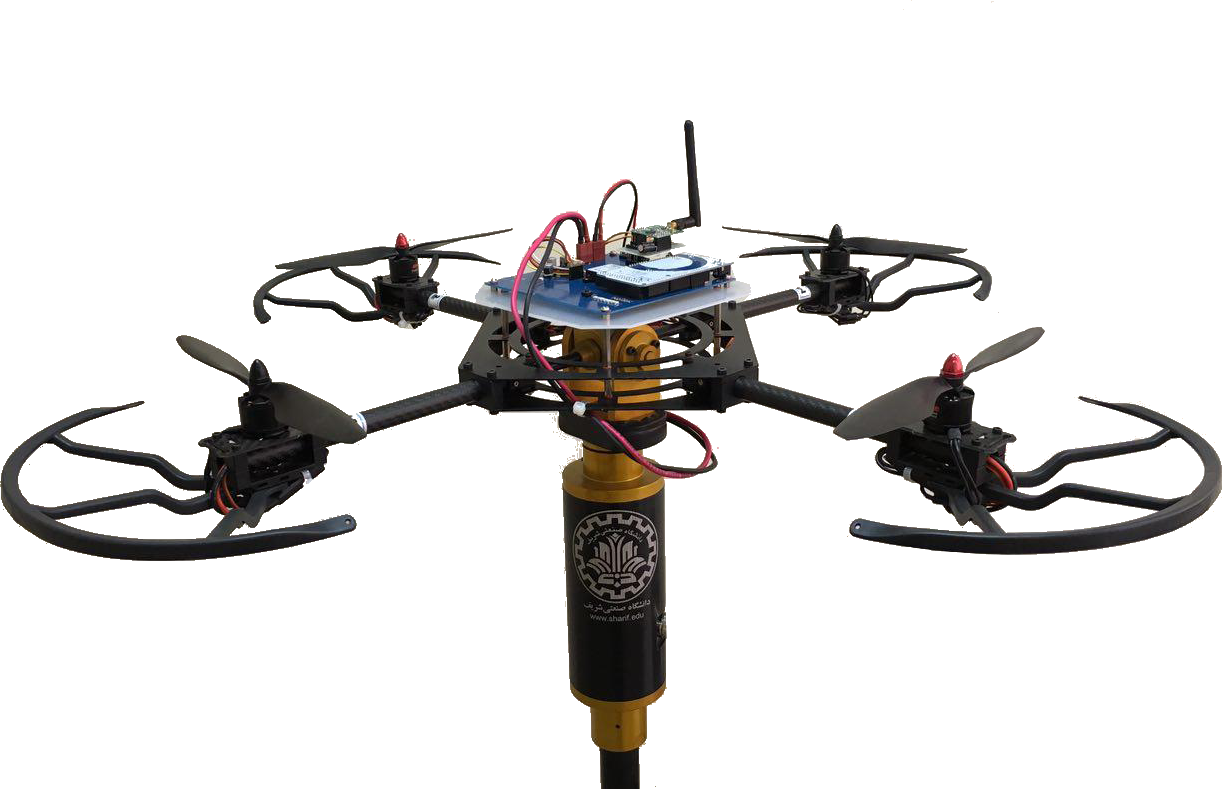
\includegraphics[width=0.7\textwidth]{../Figure/3DOFQuad.png}
   \caption{3DoF setup of the quadrotor.}
   \label{fig:quadrotor}
\end{figure}

\begin{figure}[H]
   \centering
   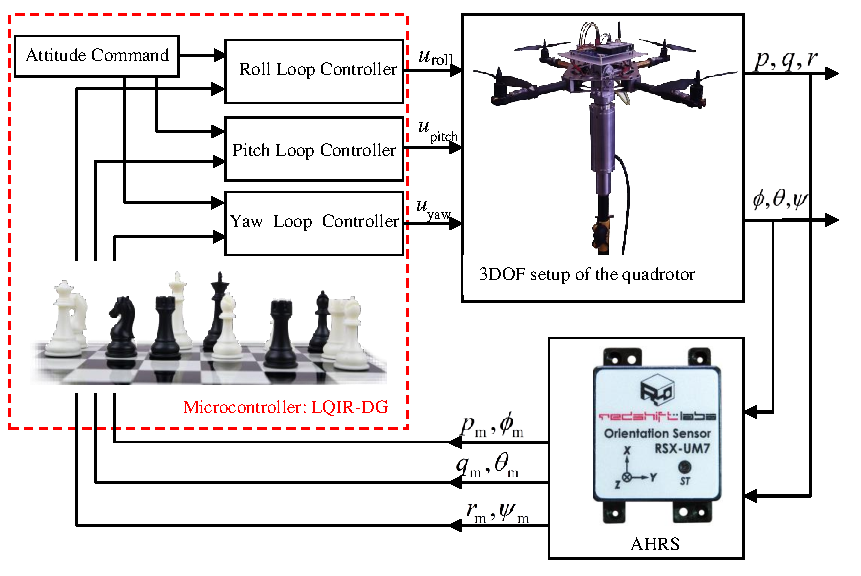
\includegraphics[width=0.7\textwidth]{../Figure/schematic.pdf}
   \caption{Structure of the LQIG-DG Controller Illustrated in a Block Diagram.}
   \label{fig:blockdiagram}
\end{figure}



\section{Dynamic Model of the Quadrotor Platform}\label{sec:modeling}
% Here, the model of the three-degree-of-freedom setup of the quadrotor is presented in detail. For this purpose, first, the configuration of the quadrotor is denoted. Then, the nonlinear model of the attitude dynamics is derived from denoting the state-space form. Finally, the nonlinear model is linearized to utilize for control purposes.
% This research paper presents an analysis of the three degrees of freedom for the quadrotor. Furthermore, a state-space model is developed to represent the nonlinear attitude dynamics. A linearization technique is subsequently applied to the model, enabling it to be used as a LQIR-DG control model.
In this section, first, a nonlinear model for the quadrotor platform is derived. Then, a state-space model and a linear model are developed for control purposes to be utilized in a controller strategy. Finally, a nonlinear identification method is applied to identify the parameters of the quadrotor.
\subsection{Quadrotor Configuration}
% condidate "Characteristics of the Quadrotor Setup"
% Figure \ref{fig:schematic} denotes the quadrotor schematic. Each rotor has an angular velocity, $\Omega_r$, rotating about the $z_B$ axis in the body coordinate system. Rotors 1 and 3 rotate counterclockwise, while rotors 2 and 4 rotate clockwise to cancel yawing moment.
% Figure \ref{fig:schematic} illustrates the quadrotor schematic, depicting four rotors with rotational velocity $\Omega_r$ rotating around the $z_B$ axis in the coordinate system of body. The rotational direction of Rotor 1 and Rotor 3 in the counterclockwise direction counteracts the yawing moment, whereas the clockwise rotation of Rotors 2 and 4 counteracts the yawing moment.

% Four rotors, each with a rotational velocity of $\Omega_r$, rotate around the $z_B$ axis. The quadrotor platform, as shown in Figure \ref{fig:schematic}, has 3 degrees of freedom, including roll, pitch, and yaw motions, which are described by roll $(\phi)$, pitch $(\theta)$, and yaw $(\psi)$ angles, respectively. The counterclockwise rotation of Rotors 1 and 3 generates a moment that counteracts the yawing moment, while the clockwise rotation of Rotors 2 and 4 produces a moment that also counteracts the yawing moment.xx

Figure \ref{fig:schematic} shows the quadrotor schematic. It depicts four rotors rotating around the $z_B$ axis in the coordinate system of the body. The rotors have a rotational velocity of $\Omega_r$.
The quadrotor platform has 3 degrees of freedom, including roll, pitch, and yaw motions, which are described by roll $(\phi)$, pitch $(\theta)$, and yaw $(\psi)$ angles, respectively.
The counterclockwise rotation of Rotors 1 and 3 generates a moment that counteracts the yawing moment, while the clockwise rotation of Rotors 2 and 4 produces a moment that also counteracts the yawing moment.

\begin{figure}[H]
    \centering
    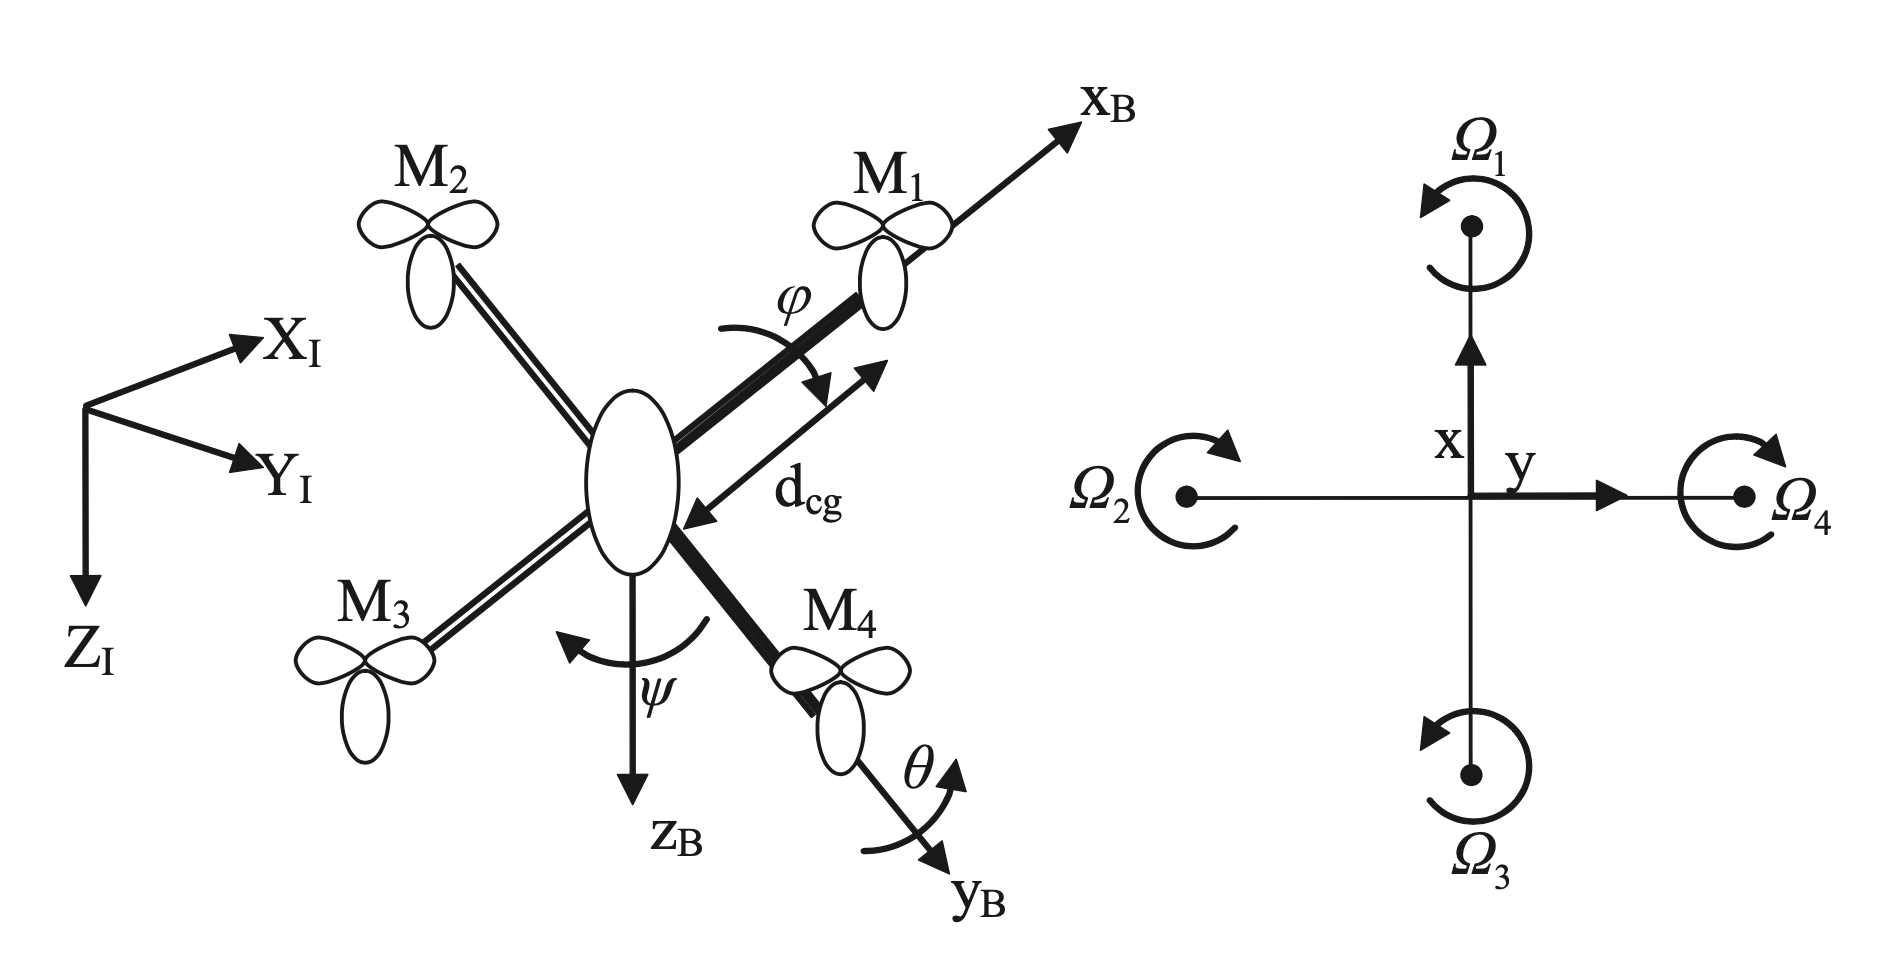
\includegraphics[width=12cm]{../Figure/schematic.png}
    \caption{Quadrotor Configuration.}
    \label{fig:schematic}
\end{figure}

\subsection{Dynamic Modeling of the Quadrotor Platfrorm}
% The quadrotor kinetic model, derived using the Newton-Euler method, is stated as \cite{4399042, article_Bouabdallah}
Here, according to Newton-Euler, the dynamic model of the quadrotor platform is derived as follows \cite{4399042, article_Bouabdallah}:



\begin{align}
    &\dot p = \dfrac{\mathrm{I}_{\text{yy}} - \mathrm{I}_{\text{zz}}}{\mathrm{I}_{\text{xx}}} qr + q \dfrac{\mathrm{I}_{\text{rotor}}}{\mathrm{I}_{\text{xx}}}\Omega_r + \dfrac{u_{\text{roll}}}{\mathrm{I}_{\text{xx}}} + \dfrac{d_{\text{roll}}}{\mathrm{I}_{\text{xx}}}
    \\
&\dot q = \dfrac{\mathrm{I}_{\text{zz}} - \mathrm{I}_{\text{xx}}}{\mathrm{I}_{\text{yy}}} rp + p \dfrac{\mathrm{I}_{\text{rotor}}}{\mathrm{I}_{\text{xx}}}\Omega_r + \dfrac{u_{\text{pitch}}}{\mathrm{I}_{\text{yy}}} + \dfrac{d_{\text{pitch}}}{\mathrm{I}_{\text{yy}}}
\\
&\dot r = \dfrac{\mathrm{I}_{\text{xx}} - \mathrm{I}_{\text{yy}}}{\mathrm{I}_{\text{zz}}} pq  +  \dfrac{u_{\text{yaw}}}{\mathrm{I}_{\text{zz}}} + \dfrac{d_{\text{yaw}}}{\mathrm{I}_{\text{zz}}}
\end{align}


% \noindent where $(p, q, r)$ are the angular velocities. $d_{\text{roll}}$, $d_{\text{pitch}}$, and $d_{\text{yaw}}$ are the disturbances generated in $x_B$, $y_B$, and $z_B$, respectively. Moreover, $\mathrm{I}_{\text{xx}}$, $\mathrm{I}_{\text{yy}}$, and $\mathrm{I}_{\text{zz}}$ are the principal moment of inertia, and $\mathrm{I}_{\text{rotor}}$ is a rotor  inertia  about its axis.
% The relation between the angular body rates and the Euler angles rates are obtained as
% \noindent The variables $(p, q, r)$ represent the rotational velocities, while the variables $d_{\text{roll}}$, $d_{\text{pitch}}$, and $d_{\text{yaw}}$ denote the disturbances produced in $x_B$, $y_B$, and $z_B$, correspondingly. Additionally, $\mathrm{I}_{\text{xx}}$, $\mathrm{I}_{\text{yy}}$, and $\mathrm{I}_{\text{zz}}$ are the principal moments of inertia, and $\mathrm{I}{\text{rotor}}$ is the rotor inertia about its axis. Euler angle rates are also determined from angular body rates:
\noindent The $(p, q, r)$ represent the rotational variables, and $d_{\text{roll}}$, $d_{\text{pitch}}$, and $d_{\text{yaw}}$ denote the disturbances produced in the $x_B$, $y_B$, and $z_B$ axes, respectively. Additionally, $\mathrm{I}_{\text{xx}}$, $\mathrm{I}_{\text{yy}}$, and $\mathrm{I}_{\text{zz}}$ are the principal moments of inertia, and $\mathrm{I}_{\text{rotor}}$ is the rotor inertia about its axis. Euler angle rates are also determined from angular body rates as follows:
% \begin{align}
%     \dot\phi &= p + (q\sin(\phi) + r\cos(\phi))\tan(\theta)\\
% \dot \theta &= q\cos(\phi) - r\sin(\phi)\\
% \dot\psi &= (q\sin(\phi) + r\cos(\phi))/{\cos(\theta)}
% \end{align}
\begin{equation}
	\begin{bmatrix}
	\dot\phi \\
	\dot\theta \\
	\dot\psi
	\end{bmatrix}
	\begin{bmatrix}
	1 & \sin(\phi)\tan(\theta) & \cos(\phi)\tan(\theta) \\
	0 & \cos(\phi) & -\sin(\phi) \\
	0 & \sin(\phi)/\cos(\theta) & \cos(\phi)/\cos(\theta)
	\end{bmatrix}
	\begin{bmatrix}
	p \\
	q \\
	r
	\end{bmatrix}
	\end{equation}
% \begin{align}
%     \begin{pmatrix}\dot{\phi} \ \dot{\theta} \ \dot{\psi}\end{pmatrix} = \begin{pmatrix}1 & \sin \phi \tan \theta & \cos \phi \tan \theta \ 0 & \cos \phi & -\sin \phi \ 0 & \frac{\sin \phi}{\cos \theta} & \frac{\cos \phi}{\cos \theta}\end{pmatrix} \begin{pmatrix}p \ q \ r\end{pmatrix}
% \end{align}
% where $(\phi, \theta, \psi)$ are roll, pitch, and yaw angles.
% Moreover, $\Omega_r$, called the overall residual rotor angular velocity, is computed as
% The quadrotor system has three degrees of freedom: roll, pitch, and yaw. The rotational motion is described by the angles $(\phi, \theta, \psi)$, which represent roll, pitch, and yaw, respectively.
 The residual rotor velocity, denoted by $\Omega_r$, is calculated as follows:
\begin{equation}
	\Omega_r = -\Omega_1 + \Omega_2 - \Omega_3 + \Omega_4
\end{equation}
\subsection{Input of the Dynamic Model}
% Control Strategy for Quadrotor

% \noindent The control inputs $u_{\text{roll}}$, $u_{\text{pitch}}$, and $u_{\text{yaw}}$ are roll, pitch, and yaw moments, obtained from the rotors, defined as
\noindent The control inputs $u_{\text{roll}}$, $u_{\text{pitch}}$, and $u_{\text{yaw}}$ are to the moments generated by the quadrotor's rotors along the roll, pitch, and yaw axes, respectively, defined as follows:
\begin{align}
		&u_{\text{roll}} = \mathrm{b\,d}_{\text{cg}} (\Omega_2^2 - \Omega_4^2)\\
	&u_{\text{pitch}} = \mathrm{b\,d}_{\text{cg}} (\Omega_1^2 - \Omega_3^2) \\
	&u_{\text{yaw}} = \mathrm{d} (\Omega_1^2 - \Omega_2^2 + \Omega_3^2 - \Omega_4^2)
\end{align}

% Also, d and b are, respectively, drag and thrust coefficients. $\mathrm{d}_{\text{cg}}$ is the distance of rotors from the gravity center. Hence, the angular velocity commands are obtained as
where $\mathrm{d}_{\text{cg}}$, $\text{d}$, and $\text{b}$ represent the distance between the rotors and the gravity center, drag factor, and thrust factor, respectively. The rotational velocity commands are computed as follows:
\begin{align}
		\Omega_{c, 1}^2 &= \Omega_{\text{mean}}^2 + \dfrac{1}{2\mathrm{b\,d}_{\text{cg}}}u_{\text{pitch}} + \dfrac{1}{4d}u_{\text{yaw}} \\
	\Omega_{c, 2}^2 &= \Omega_{\text{mean}}^2 + \dfrac{1}{2\mathrm{b\,d}_{\text{cg}}}u_{\text{roll}} - \dfrac{1}{4d}u_{\text{yaw}}\\
	\Omega_{c, 3}^2 &= \Omega_{\text{mean}}^2 - \dfrac{1}{2\mathrm{b\,d}_{\text{cg}}}u_{\text{pitch}} + \dfrac{1}{4d}u_{\text{yaw}} \\
\Omega_{c, 4}^2 &= \Omega_{\text{mean}}^2 - \dfrac{1}{2\mathrm{b\,d}_{\text{cg}}}u_{\text{roll}} - \dfrac{1}{4d}u_{\text{yaw}}
\end{align}
% where $\Omega_{\text{mean}}$ is the nominal of the rotor angular velocities.
% The nominal angular velocities of the rotors are denoted by $\Omega_{\text{mean}}$.
In the above equation, $\Omega_{\text{mean}}$ is nominal rotational velocities of the rotors.
\subsection{State-Space Formulation}\label{sec:state-space}
% \noindent Here, the state-space model is presented for control purposes.
% The formulation of a state-space model is crucial for the development of advanced control strategies. In this context, a state-space representation of the quadrotor system is provided in order to facilitate the design of control algorithms.
\noindent Here, by defining $x_1 = p$, $x_2 = q$, $x_3 = r$, $x_4 = \phi$, $x_5 = \theta$, and $x_6 = \psi$, the formulation of the quadrotor platform is presented as follows:
% For control purposes, the state-space model of the quadrotor experimental setup is described.
% By defining $x_1 = p$, $x_2 = q$, $x_3 = r$, $x_4 = \phi$, $x_5 = \theta$, and $x_6 = \psi$; the model of in state-space form are denoted as
% For the purpose of control, the quadrotor system can be modeled in state-space form as follows. Let $x_1 = p$, $x_2 = q$, $x_3 = r$, $x_4 = \phi$, $x_5 = \theta$, and $x_6 = \psi$ be the state variables. The state-space equations are given by:

% In order for the quadrotor to be controlled, it can be modelled in state-space by introducing the following variables: 


% The state-space model of the experimental setup is given as
% \begin{align}\label{eq:diffeq}
% 	\dot x_1 &= \dfrac{\mathrm{I}_{\text{yy}} - \mathrm{I}_{\text{zz}}}{\mathrm{I}_{\text{xx}}} x_2 x_3 + x_2 \dfrac{\mathrm{I}_{\text{rotor}}}{\mathrm{I}_{\text{xx}}}\Omega_r + \dfrac{u_{\text{roll}}}{\mathrm{I}_{\text{xx}}} + \dfrac{d_{\text{roll}}}{\mathrm{I}_{\text{xx}}} \\[0.5em]
% \dot x_2 &= \dfrac{\mathrm{I}_{\text{zz}} - \mathrm{I}_{\text{xx}}}{\mathrm{I}_{\text{yy}}} x_1 x_3 - x_1 \dfrac{\mathrm{I}_{\text{rotor}}}{\mathrm{I}_{\text{xx}}}\Omega_r + \dfrac{u_{\text{pitch}}}{\mathrm{I}_{\text{yy}}} + \dfrac{d_{\text{pitch}}}{\mathrm{I}_{\text{yy}}}\\[0.5em] \label{eq:diffeq-mid}
% \dot x_3 &= \dfrac{\mathrm{I}_{\text{xx}} - \mathrm{I}_{\text{yy}}}{\mathrm{I}_{\text{zz}}} x_1 x_2 + \dfrac{u_{\text{yaw}}}{\mathrm{I}_{\text{zz}}} + \dfrac{d_{\text{yaw}}}{\mathrm{I}_{\text{zz}}}\\[0.5em] 
% \dot x_4 &= x_1 + (x_2\sin(x_4) + x_3\cos(x_4))\tan(x_5)
% \\[0.5em]
% \dot x_5 &= x_2\cos(x_4) - x_3\sin(x_4)\\[0.5em]
% \dot x_6 &= (x_2\sin(x_4) + x_3\cos(x_4))/\cos(x_5) \label{eq:diffeq-end}
% \end{align}
\begin{align}\label{eq:diffeq}
	\dot x_1 &= \Gamma_1x_2 x_3 + \Gamma_2 x_2 \Omega_r + \Gamma_3u_{\text{roll}} + \Gamma_3d_{\text{roll}} \\[0.5em]
\dot x_2 &= \Gamma_4 x_1 x_3 - \Gamma_5 x_1 \Omega_r +  \Gamma_6u_{\text{pitch}} + \Gamma_6d_{\text{pitch}}\\[0.5em] \label{eq:diffeq-mid}
\dot x_3 &= \Gamma_7x_1 x_2 +  \Gamma_8u_{\text{yaw}} + \Gamma_8d_{\text{yaw}}\\[0.5em] 
\dot x_4 &= x_1 + (x_2\sin(x_4) + x_3\cos(x_4))\tan(x_5)
\\[0.5em]
\dot x_5 &= x_2\cos(x_4) - x_3\sin(x_4)\\[0.5em]
\dot x_6 &= (x_2\sin(x_4) + x_3\cos(x_4))/\cos(x_5) \label{eq:diffeq-end}
\end{align}
% where $ x_1 = p$, $ x_2 = q$, $ x_3 = r$, $ x_4 = \phi$, $ x_5 = \theta$, and $x_6 = \psi$.

% Moreover, $\Gamma_i(i=1, ..., 8)$ is defined as
% Furthermore, to facilitate the analysis, $\Gamma_i (i = 1, \ldots, 8)$ is introduced, which represents a set of coefficients related to the quadrotor's physical properties and external factors.
% where $\Gamma_i (i = 1, \ldots, 8)$ is defined as follows:
where $\Gamma_i (i = 1, \ldots, 8)$ is defined as:
\begin{equation}
	\begin{split}
		\Gamma_1 &= \dfrac{\mathrm{I}_{\text{yy}} - \mathrm{I}_{\text{zz}}}{\mathrm{I}_{\text{xx}}}, \quad \Gamma_2 = \dfrac{\mathrm{I}_{\text{rotor}}}{\mathrm{I}_{\text{xx}}}, \quad \Gamma_3 = \dfrac{1}{\mathrm{I}_{\text{xx}}}\\ \Gamma_4 &= \dfrac{\mathrm{I}_{\text{zz}} - \mathrm{I}_{\text{xx}}}{\mathrm{I}_{\text{yy}}}, \quad \Gamma_5 = \dfrac{\mathrm{I}_{\text{rotor}}}{\mathrm{I}_{\text{xx}}}, \quad \Gamma_6 = \dfrac{1}{\mathrm{I}_{\text{yy}}} \\ \Gamma_7 &= \dfrac{\mathrm{I}_{\text{xx}} - \mathrm{I}_{\text{yy}}}{\mathrm{I}_{\text{zz}}}, \quad \Gamma_8 = \dfrac{1}{\mathrm{I}_{\text{zz}}}
	\end{split}
\end{equation}
Moreover, the measurement vector, obtained from the AHRS sensor is presented as follows:
% The measurement model is written as
% The attitude states and gyro measurements are represented as vectors, denoted by $\boldsymbol{\mathrm{z}}$ and $\boldsymbol{\mathrm{m}}$, respectively. The attitude state vector is defined as follows:

\begin{equation}
\begin{split}
\boldsymbol{\mathrm{z}} &= \begin{bmatrix}
p \
q \
r \
\phi \
\theta \
\psi
\end{bmatrix}^\mathrm{T} + \nu
\end{split}
\end{equation}
where $\nu$ is a Gaussian white noise. In the above equation, the superscripts $\mathrm{T}$ indicate the transpose notation.
\subsection{Linear Model}
% \noindent The continuous-time linear model is utilized to drive the control commands on the quadrotor. The linear state-space model is denoted as
\noindent The linear continuous-time model of the quadrotor platform about the equilibrium points $(\boldsymbol{{\mathrm{x}}}_e!=!0$ and $\boldsymbol{{\mathrm{u}}}_e!=!0)$ is represented as:
\begin{equation}\label{eq:linear}
	\boldsymbol{\dot{\mathrm{x}}}(t) = \boldsymbol{\mathrm{A\,x}}(t) + \boldsymbol{\mathrm{B\,u}}(t) + \boldsymbol{\mathrm{B_{d}\,d}}(t)
\end{equation}
where $\boldsymbol{\dot{\mathrm{x}}} = \begin{bmatrix}
				\boldsymbol{{\mathrm{\dot x_{\text{roll}}}}}&
				\boldsymbol{{\mathrm{\dot x_{\text{pitch}}}}}&
				\boldsymbol{{\mathrm{\dot x_{\text{yaw}}}}}
\end{bmatrix}$, defined as:
\begin{equation}
	\begin{split}
		\boldsymbol{\mathrm{x}}_{\text{roll}} = \begin{bmatrix}
			p \\ \phi
		\end{bmatrix}, \quad
		\boldsymbol{\mathrm{x}}_{\text{pitch}} = \begin{bmatrix}
			q \\ \theta \end{bmatrix} \quad
		\boldsymbol{\mathrm{x}}_{\text{yaw}} = 
		\begin{bmatrix}
			r \\ \psi
		\end{bmatrix}
	\end{split}
\end{equation}
% where $\boldsymbol{\mathrm{A}}$, $\boldsymbol{\mathrm{B}}$, and $\boldsymbol{\mathrm{B_d}}$ are the system, input and disturbance matrices, respectively. Moreover, $\boldsymbol{\mathrm{d}}$ is the disturbance. The measurements equation is stated as
where $\boldsymbol{\mathrm{A}}$ is the dynamic system matrix, denoted as:
\begin{equation}
	\boldsymbol{\mathrm{A}} = \begin{bmatrix}
		\boldsymbol{{\mathrm{A_{\text{roll}}}}} & \boldsymbol{0} & \boldsymbol{0}\\
		\boldsymbol{0} & \boldsymbol{{\mathrm{A_{\text{pitch}}}}} & \boldsymbol{0} \\
		\boldsymbol{0} & \boldsymbol{0} & \boldsymbol{{\mathrm{A_{\text{yaw}}}}}
	\end{bmatrix}
\end{equation}
Moreover, $\boldsymbol{\mathrm{B}}$ and $\boldsymbol{\mathrm{B_d}}$ are the input and disturbance matrices, respectively, and are defined as:
\begin{equation}
	\boldsymbol{\mathrm{B}} = \boldsymbol{\mathrm{B_d}} = 
	\begin{bmatrix}
		\boldsymbol{{\mathrm{B_{\text{roll}}}}} & \boldsymbol{0} & \boldsymbol{0}\\
		\boldsymbol{0} & \boldsymbol{{\mathrm{B_{\text{pitch}}}}} & \boldsymbol{0} \\
		\boldsymbol{0} & \boldsymbol{0} & \boldsymbol{{\mathrm{B_{\text{yaw}}}}}
	\end{bmatrix}
\end{equation}

% The system's dynamics are represented by the matrix $\boldsymbol{\mathrm{A}}$, which includes the input matrix $\boldsymbol{\mathrm{B}}$ and disturbance matrix $\boldsymbol{\mathrm{B_d}}$. The disturbance is represented by the matrix $\boldsymbol{\mathrm{d}}$.
% The measurement equation is given by
% \begin{equation}
% 	\boldsymbol{{\mathrm{z}}}(t) = \boldsymbol{\mathrm{x}}(t)
% \end{equation}
% According to equations\eqref{eq:diffeq}-\eqref{eq:diffeq-end}, the linear dynamic model around the equilibrium points $(\boldsymbol{{\mathrm{x}}}_e\!=\!0 \text{ and } \boldsymbol{{\mathrm{u}}}_e\!=\!0)$ of the Quadrotor Platrorm is denoted as
% The linear dynamic model, which is derived around the equilibrium points $(\boldsymbol{{\mathrm{x}}}_e\!=\!0 \text{ and } \boldsymbol{{\mathrm{u}}}_e\!=\!0)$ of the Quadrotor Platrorm, is described by equations\eqref{eq:diffeq}-\eqref{eq:diffeq-end}.
% The differential equations presented in Equations \eqref{eq:diffeq}-\eqref{eq:diffeq-end} allow for the development of a corresponding linear dynamic model for the quadrotor platform at its equilibrium points $(\boldsymbol{{\mathrm{x}}}_e\!=\!0 \text{ and } \boldsymbol{{\mathrm{u}}}_e\!=\!0)$. This model can be expressed as follows:
% \begin{equation}
% 	\begin{split}
% 		\boldsymbol{{\mathrm{\dot x}}} = \begin{bmatrix}
% 			\boldsymbol{{\mathrm{\dot x_{\text{roll}}}}}\\
% 			\boldsymbol{{\mathrm{\dot x_{\text{pitch}}}}}\\
% 			\boldsymbol{{\mathrm{\dot x_{\text{yaw}}}}}
% 		\end{bmatrix} &= \begin{bmatrix}
% 			\boldsymbol{{\mathrm{A_{\text{roll}}}}} & \boldsymbol{0} & \boldsymbol{0}\\
% 			\boldsymbol{0} & \boldsymbol{{\mathrm{A_{\text{pitch}}}}} & \boldsymbol{0} \\
% 			\boldsymbol{0} & \boldsymbol{0} & \boldsymbol{{\mathrm{A_{\text{yaw}}}}}
% 		\end{bmatrix} \begin{bmatrix}
% 			\boldsymbol{{\mathrm{x_{\text{roll}}}}}\\
% 			\boldsymbol{{\mathrm{x_{\text{pitch}}}}}\\
% 			\boldsymbol{{\mathrm{x_{\text{yaw}}}}}
% 		\end{bmatrix}
% 		\\[1em]
% 		& + \begin{bmatrix}
% 			\boldsymbol{{\mathrm{B_{\text{roll}}}}} & \boldsymbol{0} & \boldsymbol{0}\\
% 			\boldsymbol{0} & \boldsymbol{{\mathrm{B_{\text{pitch}}}}} & \boldsymbol{0} \\
% 			\boldsymbol{0} & \boldsymbol{0} & \boldsymbol{{\mathrm{B_{\text{yaw}}}}}
% 		\end{bmatrix}
% 		\begin{bmatrix}
% 			\boldsymbol{{\mathrm{u_{\text{roll}}}}}\\
% 			\boldsymbol{{\mathrm{u_{\text{pitch}}}}}\\
% 			\boldsymbol{{\mathrm{u_{\text{yaw}}}}}
% 		\end{bmatrix}\\[1em]
% 		& + \begin{bmatrix}
% 			\boldsymbol{{\mathrm{B_{\text{roll}}}}} & \boldsymbol{0} & \boldsymbol{0}\\
% 			\boldsymbol{0} & \boldsymbol{{\mathrm{B_{\text{pitch}}}}} & \boldsymbol{0} \\
% 			\boldsymbol{0} & \boldsymbol{0} & \boldsymbol{{\mathrm{B_{\text{yaw}}}}}
% 		\end{bmatrix} \begin{bmatrix}
% 			\boldsymbol{{\mathrm{d_{\text{roll}}}}}\\
% 			\boldsymbol{{\mathrm{d_{\text{pitch}}}}}\\
% 			\boldsymbol{{\mathrm{d_{\text{yaw}}}}}
% 		\end{bmatrix}
% 	\end{split}
% \end{equation}
% where $\boldsymbol{\mathrm{x}}_{\text{roll}}$, 
% $\boldsymbol{\mathrm{x}}_{\text{pitch}}$, and $\boldsymbol{\mathrm{x}}_{\text{yaw}}$ defined as below:

In addition, the input matrices and state are shown as:
\begin{equation}
	\begin{split}
		\boldsymbol{\mathrm{A}}_{\text{roll}}  =\boldsymbol{\mathrm{A}}_{\text{pitch}}  = \boldsymbol{\mathrm{A}}_{\text{yaw}}  = \begin{bmatrix}
			0 & 0\\
			1 & 0
		\end{bmatrix}
	\end{split}
\end{equation}

\begin{equation}
	\begin{split}
		\boldsymbol{\mathrm{B}}_{\text{roll}}  = \begin{bmatrix}
			\dfrac{1}{\mathrm{I}_{\text{xx}}}
			\\[1em]
			0
		\end{bmatrix};~ \boldsymbol{\mathrm{B}}_{\text{pitch}}  = \begin{bmatrix}
			\dfrac{1}{\mathrm{I}_{\text{yy}}}
			\\[1em]
			0
		\end{bmatrix};~ \boldsymbol{\mathrm{B}}_{\text{yaw}}  = \begin{bmatrix}
			\dfrac{1}{\mathrm{I}_{\text{zz}}}
			\\[1em]
			0
		\end{bmatrix}
	\end{split}
\end{equation}

\subsection{Identification of the Platform Parameters}
% \noindent In this section, the optimization technique based on the Nonlinear Least Squares (NLS) method is utilized to estimate the model parameters ($\Gamma$) for the 3DOF experimental setup from
% experimental data. Here, the NLS algorithm, that is based on the trust-region reflective least squares (TRRLS) method, finds iteratively the values of the model parameters based on the minimization of the cost function, so that the input/output signals provided by the simulation model are very similar to the experimental ones. Therefore, the least squares problem consists
% in finding a vector $\boldsymbol{\mathrm{\Gamma}}$ that minimizes a sum of squares function \cite{article_Eriksson}, as follows:
\noindent This section describes the utilization of the Nonlinear Least Squares (NLS) algorithm for estimating the model parameters ($\boldsymbol{\mathrm{\Gamma}}$) of the 3DoF experimental platform using experimental data. This technique is based on the Trust-Region Reflective Least Squares (TRRLS) method, which iteratively finds the values of the model parameters by minimizing a cost function, defined as follows:
\begin{equation}
	\min_{\Gamma_i}\left(\parallel e(\Gamma_i) \parallel^2\right) = 
	\min_{\Gamma_i} = \left(\sum_{j=1}^{n}(\boldsymbol{z}_j- \hat{\boldsymbol{z}}_j)(\boldsymbol{z}_j- \hat{\boldsymbol{z}}_j)^\mathrm{T}\right)
\end{equation}
where $\boldsymbol{z}$ and $\hat{\boldsymbol{z}}$ are the experimental and simulated output signals, when the same input signals are applied ones.
The structure of the proposed identification approach is illustrate in figure \ref{fig:identification}

%  an optimization technique for estimating the model parameters  of the 3DOF experimental setup from experimental data. The technique is based on the Nonlinear Least Squares (NLS) method, which is widely used in parameter estimation problems. The NLS algorithm utilizes the trust-region reflective least squares (TRRLS) method to iteratively find the values of the model parameters. The goal is to minimize a cost function, which is based on the sum of squares between the input/output signals provided by the simulation model and the experimental ones.

% The optimization process involves finding a vector $\boldsymbol{\mathrm{\Gamma}}$ that minimizes the cost function. This is achieved by iteratively updating the values of the model parameters until convergence is achieved. The NLS method is particularly useful for problems where the model is nonlinear and the measurement noise is known. The approach is based on a least squares problem, where the objective is to find the values of $\boldsymbol{\mathrm{\Gamma}}$ that minimize the sum of squares function \cite{article_Eriksson}:

% The optimization process involves finding a vector $\boldsymbol{\mathrm{\Gamma}}$ by iteratively updating the values of the model parameters until convergence is achieved.
%  The NLS method is particularly useful for problems where the model is nonlinear and the measurement noise is known. The approach is based on a least squares problem, where the objective is to find the values of $\boldsymbol{\mathrm{\Gamma}}$ that minimize the sum of squares function \cite{article_Eriksson}:




% In summary, the NLS optimization technique is an effective approach for estimating the model parameters of the 3DOF experimental setup from experimental data. The technique utilizes the TRRLS method to iteratively update the values of the model parameters, with the goal of minimizing the difference between the simulation model and the experimental data \cite{article_Eriksson}.


\begin{figure}[H]
	\centering
	\begin{tikzpicture}[font=\small,thick]
		% Start block
		\node[draw, align=center,		minimum width=2.5cm,		minimum height=1cm, fill=blue!10] (block1) {\textbf{Experimental Data} \\Input: rotational velocity\\
		Output: attitude};
			
		% Voltage and Current Measurement
		\node[draw, align=center,		below=of block1,		minimum width=3.5cm,		minimum height=1cm, fill=blue!10	] (block2) {\textbf{Data Preprocessing} \\ Synchronization experimental, vs simulated data.};
		
		% Power and voltage variation
		
		\node[draw, align=center,		below=of block2,		minimum width=3.5cm,		minimum height=1cm, fill=blue!10	] (block3) {\textbf{NLS-TRRLS Optimization}\\
		Set bounds for parameters.\\ %%%?
		Set initial seed for all parameters.\\
		Minimization of the cost function.};

		\node[draw, align=center,	below right=of block3,	minimum width=3cm,	minimum height=2.5cm,	fill=green!10	] (block_p) {{Identified parameters}\\
		$\boldsymbol\Gamma = \begin{bmatrix}\Gamma_1 &
			\Gamma_2 & \Gamma_3 & \Gamma_4\\
			\Gamma_5 & \Gamma_6 & \Gamma_7 & \Gamma_8
		\end{bmatrix}$};

		\node[draw, align=center,	below left=of block3,	minimum width=3cm,	minimum height=2.5cm,	fill=red!10	] (block_s) {{simulated model}\\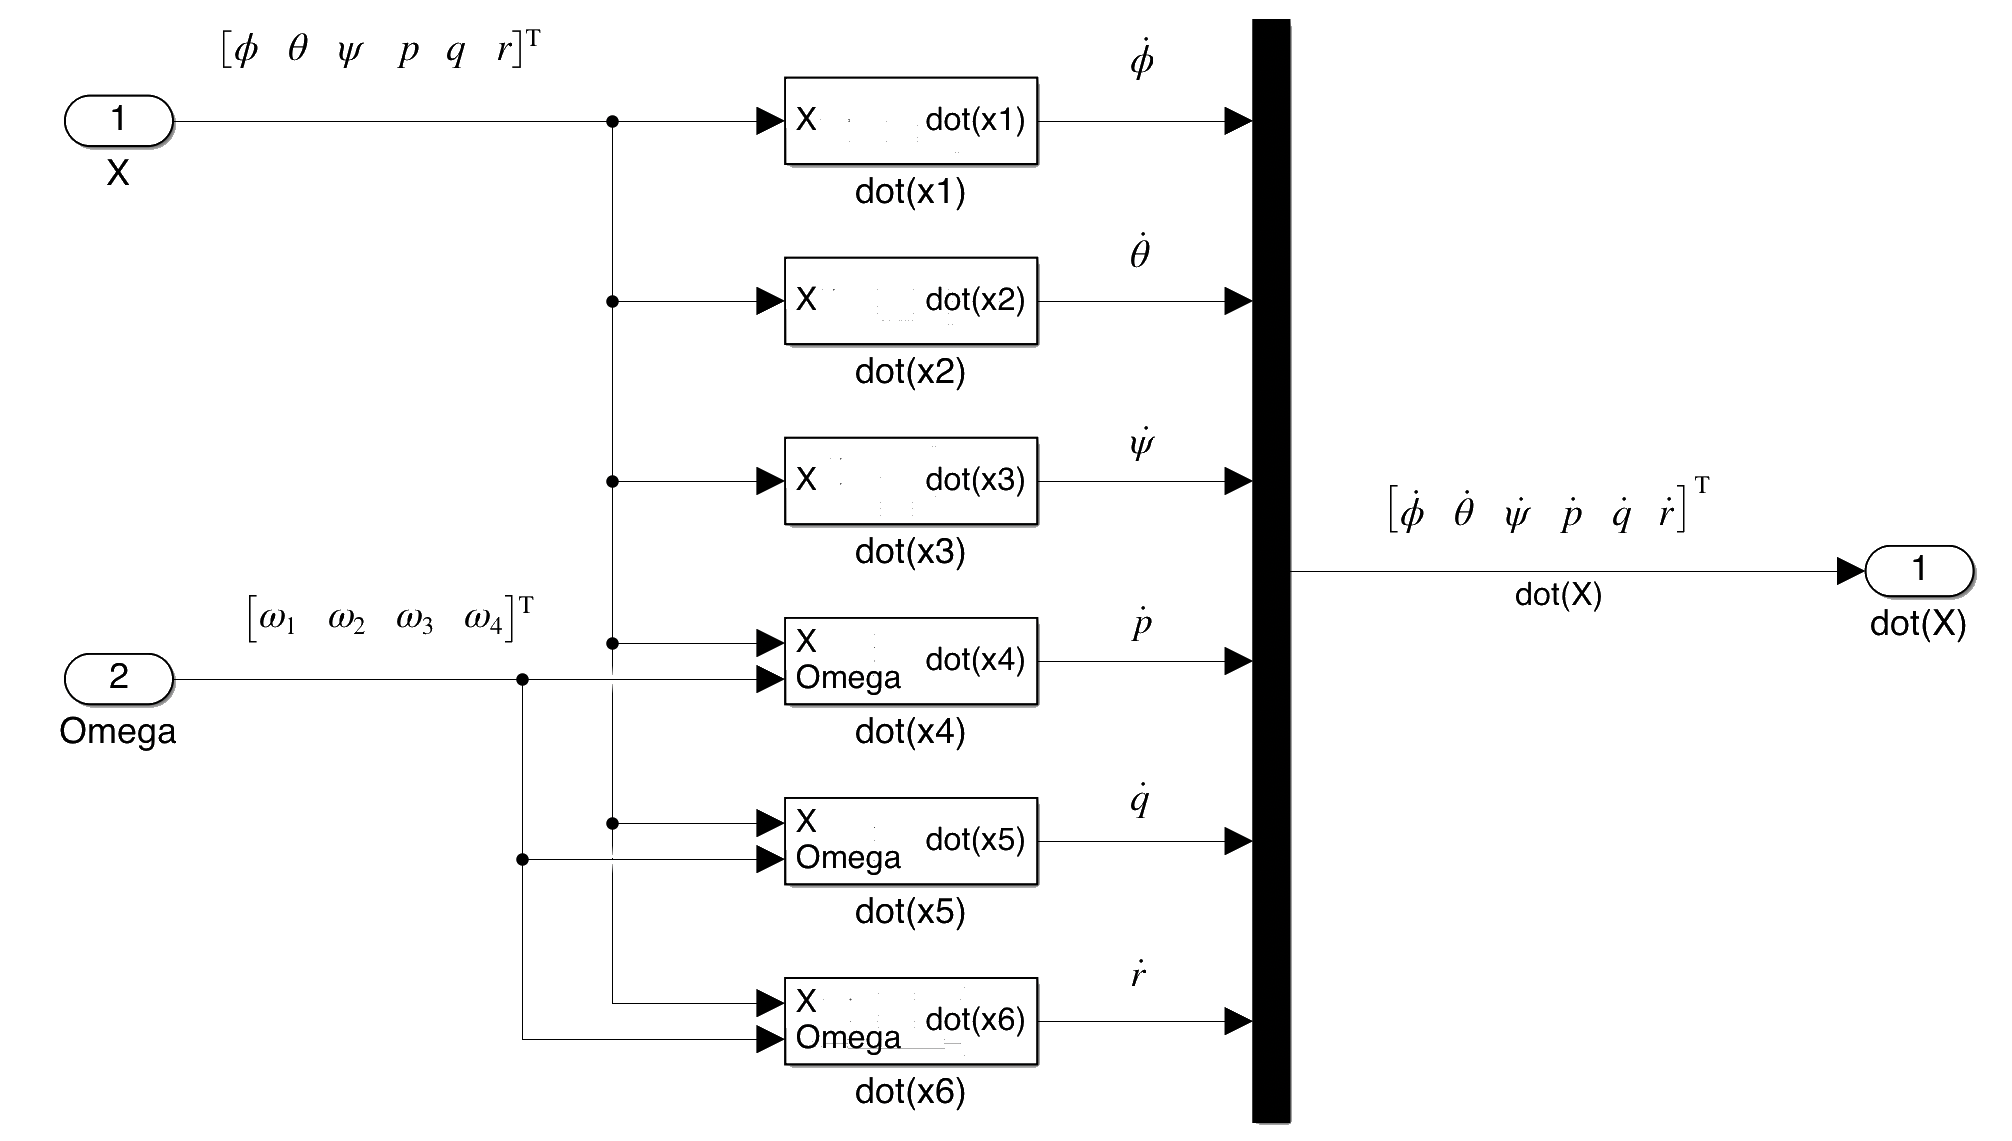
\includegraphics[scale=.05]{../Figure/All-six.png}};
		
		% Conditions test
		\node[draw,		diamond,		below =4cm of block3,		minimum width=2.5cm,		inner sep=0,		fill=yellow!10	] (block4) { Error $< \delta$};
		
		\node[draw,		below=1.5cm of block4,		minimum height=1cm,		minimum width=2.5cm,		inner sep=0,		fill=blue!10	] (block5) {End};
		
		\node[draw,		right=2cm of block4,		minimum height=1cm,		minimum width=2.5cm,		fill=red!10		] (block6) {Insufficient experimental data};
				
		 
		 
		% Arrows
		\draw[-latex] (block1) edge (block2)
			(block2) edge (block3)
			(block3) -| (block_s);
			% (block3) edge (block_p);
	
		\draw[-latex] (block3) -| (block_p);
	
		\draw[-latex] (block_s) -| (block4);
	
		\draw[-latex] (block_p) -| (block4);
	
		\draw[stealth-stealth] (block_s) -- (block_p);
		 
		\draw[-latex] (block4) -- (block5)
			node[pos=0.5,fill=white,inner sep=0]{Yes};
		 
		\draw[-latex] (block4) -- (block6)
			node[pos=0.5,fill=white,inner sep=0]{No};
	
		\coordinate[left=5.5cm of block3] (aux);
		\coordinate[right= of block_p] (aux1);
		% \draw[-latex] (block6) |- (block2);
		\draw[-latex] (block1) -| (aux) |- (block4);
		\draw[-latex] (block6) -| (aux1) |- (block1);
		\end{tikzpicture}
		\caption{Structure of TRRLS identification approach.}
		\label{fig:identification}
\end{figure}

\section{Structure of the LQDG Controller}\label{sec:controller}
% \noindent In the LQIR-DG controller structure, an integral action is added to the LQR-DG controller to cancel the steady-state errors for reference tracking. For this purpose, first, the augmented state space of the linear quadrotor model is defined to utilize in the controller architecture. Then, the LQR-DG controller design procedure is presented to produce the best control commands for the experimental setup of the quadrotor.

% \noindent Here, the LQR-DG controller is augmented with an integral action to eliminate steady-state errors in desired following. The first stage of the controller design process entails the development of the augmented state space representation of the quadrotor system to integrate it into the broader control framework. Subsequently, the design methodology of LQR-DG controller is introduced to generate optimal control signals for the three-degree-of-freedom platform.
\noindent Here, the LQR-DG controller is augmented with an integral action to eliminate steady-state errors. For this purpose, the augmented states of the quadrotor platform, which include states and their integrals, are selected. The design methodology of the LQR-DG controller is introduced. It generates optimal control signals for the three degrees of freedom platform.

\subsection{Augmented State Space Development}
\noindent To integrate the integrator into the control strategy architecture, the augmented state variables are defined below:
\begin{equation}\label{lqidg_x}
    \boldsymbol{\mathrm{x_{a_i}}} = \begin{bmatrix}
        \boldsymbol{\mathrm{x_i}} \\[1em]
        \displaystyle\int\boldsymbol{\mathrm{x_i}}
    \end{bmatrix}
\end{equation}
% where $i$ = roll, pitch, and yaw.
% Then, the quadrotor dynamics model, denoted by Eq.\eqref{eq:linear}, is denoted in the augmented state-space model as
The dynamics model of the quadrotor, as expressed by Eq. \eqref{eq:linear}, is reformulated into an augmented state-space model that incorporates the roll ($\phi$), pitch ($\theta$), and yaw ($\psi$) angles. The augmented state-space model provides a comprehensive description of the quadrotor's dynamic behavior, enabling the design of effective control strategies. The ensuing state-space model that integrates the augmented state variables is mathematically represented and defined in the following manner:

\begin{equation}\label{systemlqidg}
	\begin{split}
		\boldsymbol{\dot{\mathrm{x}}_a}(t) &= \boldsymbol{\mathrm{A_ax_a}}(t) + \boldsymbol{\mathrm{B_{{a}}u}}(t) + \boldsymbol{\mathrm{B_{{d_a}}d}}(t)%, \quad \boldsymbol{x}(0) = 
	\end{split}
\end{equation}
$\boldsymbol{\mathrm{B_a}}$ and $\boldsymbol{\mathrm{A_a}}$, which are expressed as below:

\begin{equation}
	\boldsymbol{\mathrm{B_a}} = \boldsymbol{\mathrm{B_{{d_a}}}} = \begin{bmatrix}
		\boldsymbol{\mathrm{B}}\\
		\boldsymbol{0}
	\end{bmatrix}
\end{equation}

\begin{equation}
	\boldsymbol{\mathrm{A_a}} = \begin{bmatrix}
		\boldsymbol{\mathrm{A}} & \boldsymbol{0}\\
		\boldsymbol{\mathrm{I}} & \boldsymbol{0}
	\end{bmatrix}
\end{equation}
% In the above equation $\boldsymbol{\mathrm{I}}$ denotes the identity matrix.
In the aforementioned expression, the notation $\boldsymbol{\mathrm{I}}$ denotes the identity matrix.

\subsection{LQR-DG Control Scheme with Integral Action}
% \noindent The LQIR-DG controller is an optimal and robust method based on the differential game theory. This controller consists of two essential players: one finds the best control command, and the other creates the worst disturbance. 
% For this purpose, the first player tries to minimize a cost function, while the second is assumed to maximize it. Therefore, the quadratic cost function equation is denoted using min-max operators as follows:
% \noindent In accordance with the principles of differential game theory, the LQIR-DG is a robust and optimal controller. This controller involves two fundamental players, one of which is responsible for determining the optimal control command, while the other strives to generate the worst possible disturbance. The primary objexctive of the premier player is to optimize a cost function through minimization, whereas the other player seeks to optimize the same cost function through maximization. The cost function with a quadratic form can be expressed using the min-max operator, as demonstrated below:

% \noindent In accordance with the principles of differential game theory, the LQIR-DG is a robust and optimal controller. In the LQIR-DG scheme, two fundamental players, primary for determining the control command, another for generating the worst possible disturbance are selected. To active the primary objective, the primary player must minimize the following cost function, but the other player maximize it:

\noindent In line with the principles of differential game theory, the LQIR-DG controller is designed to be both robust and optimal. The LQIR-DG scheme involves selecting two fundamental players, one responsible for determining the control command and the other for generating the worst possible disturbance. To achieve the primary objective, the primary player minimizes the following cost function, while the other player must maximize it:

\begin{equation}
    \min_{u} \max_{d} J(\boldsymbol{\mathrm{x_{a_i}}}, {d_i}, {u_i}) = J(\boldsymbol{\mathrm{x_{a_i}}}, {u^*_i}, {d^*_i})=\min_{d} \max_{u}
     \int_{0}^{\mathrm{t_f}}\biggl (\boldsymbol{\mathrm{x^\mathrm{T}_{a_i}}}  \boldsymbol{\mathrm{Q_i}} \boldsymbol{\mathrm{x_{a_i}}}+
    {{u^\mathrm{T}_i}}  {{R}} {{u_i}}-
    {{d^\mathrm{T}_{i}}} {{ R_{d} d_{i}}}
    \biggl )\mathrm{d}t
\end{equation}
% where ${{ R}}$ and ${{R_{d}}}$ are symmetric nonnegative definite matrices and $\boldsymbol{\mathrm{Q_i}} $ is a symmetric positive definite matrix.  Moreover, $\mathrm{t_f}$ is the final time. To solve this problem, connections between the general optimal problem and the LQIR problem are considered \cite{LQDG}. Consequently, the optimum control effort is computed for each control loop as follows:
% In the aforementioned equation, the matrix $\boldsymbol{\mathrm{Q_i}}$ is a definite positive symmetric matrix, while ${{R_{d}}}$ and ${{R}}$ are nonnegative definite symmetric matrices. The final time is denoted by $\mathrm{t_f}$. In order to address this concern, a connection between the comprehensive optimal control framework and the LQIR problem has been established, as previously discussed in the relevant literature \cite{LQDG}. As a result, the optimal control input for each control loop can be computed using the following formula: 
where $\boldsymbol{\mathrm{Q_i}}$, ${{R_{d}}}$, and ${{R}}$ are weight coefficients of the function. The final time is denoted by $\mathrm{t_f}$.
By solving the above problem, the control command is computed as follows \cite{LQDG}:
\begin{equation}
	{{d_i}}(t) =\boldsymbol{{\mathrm{K_{d_i}}}}(t)\boldsymbol{{\mathrm{x_{a_i}}}}(t)
\end{equation}
Moreover, the worst disturbance is obtained as:
\begin{equation}
		{{u_i}}(t) = -\boldsymbol{{\mathrm{K}}_{i}}(t) \boldsymbol{{\mathrm{x_{a_i}}}}(t)
\end{equation}
Here, $\boldsymbol{{\mathrm{K_{d_i}}}}$ and $\boldsymbol{{\mathrm{K_i}}}$ are gain values defined as follows:
\begin{align}
	\boldsymbol{{\mathrm{K_i}}} &= {{{R}}^{-1}}\boldsymbol{{\mathrm{B}_{a_i}^\mathrm{T}}}\boldsymbol{{\mathrm{P}}_{a_i}}(t)\\
	\boldsymbol{{\mathrm{K_{d_i}}}} &= {{{R}}^{-1}_{d}}\boldsymbol{{\mathrm{B}_{a_{d_i}}^\mathrm{T}}}\boldsymbol{{\mathrm{P}}_{a_{d_i}}}(t)
\end{align}
where $\boldsymbol{{\mathrm{P}}_{a_i}}(t)$ and $\boldsymbol{{\mathrm{P}}_{a_{d_i}}}(t)$ satisfy
\begin{align}\label{coupled_riccatti_LQIDG}
	&-\boldsymbol{\mathrm{A^\mathrm{T}_a}}\boldsymbol{\mathrm{P_{a_{d_i}}}}(t)
	 - \boldsymbol{\mathrm{Q_{i}}} - \boldsymbol{\mathrm{P_{a_{d_i}}}}(t)\boldsymbol{\mathrm{A_a}} 
	 + \boldsymbol{\mathrm{P_{a_{d_i}}}}(t)\boldsymbol{\mathrm{S_{a_i}}}(t)\boldsymbol{\mathrm{P_{a_i}}}(t)
	  +\boldsymbol{\mathrm{P_{a_{d_i}}}}(t)\boldsymbol{\mathrm{S_{a_{d_i}}}}(t)\boldsymbol{\mathrm{P_{a_{d_i}}}}(t)
	=\boldsymbol{\mathrm{0}}\\
            &-\boldsymbol{\mathrm{A^\mathrm{T}_a}}\boldsymbol{\mathrm{P_{a_i}}}(t) - \boldsymbol{\mathrm{Q_i}}
			 - \boldsymbol{\mathrm{P_{a_i}}}(t)\boldsymbol{\mathrm{A_a}}  +
			  \boldsymbol{\mathrm{P_{a_i}}}(t)\boldsymbol{\mathrm{S_{a_{d_i}}}}(t)\boldsymbol{\mathrm{P_{a_{d_i}}}}(t) 
			  +\boldsymbol{\mathrm{P_{a_i}}}(t)\boldsymbol{\mathrm{S_{a_i}}}(t)\boldsymbol{\mathrm{P_{a_i}}}(t) =\boldsymbol{\mathrm{0}}
\end{align}
% where $\boldsymbol{\mathrm{S_{a_i}}} = \boldsymbol{\mathrm{B_{a_i}}}R^{-1}\boldsymbol{\mathrm{B}^\mathrm{T}_{a_i}}$ and $\boldsymbol{\mathrm{S_{a_{d_i}}}} = \boldsymbol{\mathrm{B}_{a_{d_i}}}R_{d}^{-1}\boldsymbol{\mathrm{B}^\mathrm{T}_{a_{d_i}}}$.
% In the present study, the feedback control law is generated using the steady-state values of the aforementioned equations as $\mathrm{t_f}$ tends to infinity.

% In this study, the feedback control law is developed using the asymptotic behavior of the equations as $t_f$ approaches infinity. The matrices $\boldsymbol{\mathrm{S_{a_i}}}$ and $\boldsymbol{\mathrm{S_{a_{d_i}}}}$ are determined by utilizing the matrices $\boldsymbol{\mathrm{B_{a_i}}}$ and $\boldsymbol{\mathrm{B_{a_{d_i}}}}$ along with the symmetric nonnegative definite matrices ${{ R}}$ and ${{R_{d}}}$. Specifically, $\boldsymbol{\mathrm{S_{a_i}}}$ is defined as $\boldsymbol{\mathrm{B_{a_i}}}R^{-1}\boldsymbol{\mathrm{B}^\mathrm{T}_{a_i}}$, while $\boldsymbol{\mathrm{S{a_{d_i}}}}$ is defined as $\boldsymbol{\mathrm{B}_{a_{d_i}}}R_{d}^{-1}\boldsymbol{\mathrm{B}^\mathrm{T}_{a_{d_i}}}$.
where $$
	\boldsymbol{\mathrm{S_{a_i}}} = \boldsymbol{\mathrm{B_{a_i}}}R^{-1}\boldsymbol{\mathrm{B}^\mathrm{T}_{a_i}}, \quad
	\boldsymbol{\mathrm{S{a_{d_i}}}} = \boldsymbol{\mathrm{B}_{a_{d_i}}}R_{d}^{-1}\boldsymbol{\mathrm{B}^\mathrm{T}_{a_{d_i}}}
$$
% In this study, the steady-state values of the above equations $(\boldsymbol{{\mathrm{P}}} \text{ as } \mathrm{t_f} \to \infty)$ are utilized to generate a feedback control law.

\section{Result and Discussion}\label{sec:results}


% \noindent Here, the results of the LQIR-DG controller method are devoted to the control loops of the roll, pitch, and yaw of the experimental setup of the quadrotor. First, the controller parameters are tuned using the results of numerical simulations. Moreover, the performance of the LQIR-DG controller is compared to an LQR, PID, LQIR control strategy. The quadrotor parameters are shown in table \ref{tab:parameters}.
% \noindent Here, the study presents the results of applying the LQIR-DG controller method to the control loops of roll, pitch, and yaw of an experimental quadrotor setup. To ensure optimal and robust performance, the controller parameters are tuned using the results of numerical simulations. Additionally, the study compares the performance of the LQIR-DG controller to that of other controllers, including LQR, PID, and LQIR control strategies. The quadrotor's parameters are detailed in Table \ref{tab:parameters}.

% Moreover, the parameters of LQIR-DG controller weight are denoted in table \ref{tab:control weight_new}.

% \noindent The current study presents an investigation of the effectiveness of the LQIR-DG control approach in the regulation of an experimental quadrotor platform's roll, pitch, and yaw movements.Numerical simulations are used to tune the parameters of the controller to achieve optimal and resilient performance. The comparative performance analysis of the LQIR-DG controller is carried out with respect to other control strategies, namely LQR, PID, and LQIR. The quadrotor's parameters are listed in Table \ref{tab:parameters}.

% Furthermore, the weighting coefficients of the LQIR-DG controller are provided in Table \ref{tab:control weight_new}.
\noindent Here, the simulation results of parameter identification and LQIDG-Controller for a quadrotor platform are presented. First, the quadrotor parameters are estimated based on the NLS method. Then, the performance of the LQDG controller structure is evaluated. The performance of the quadrotor LQIDG controller is presented in Tables \ref{tab:parameters} and \ref{tab:control weight_new}.

\begin{table}[H]
	\renewcommand{\arraystretch}{1.3}
	\caption{Quadrotor Parameters}
	\begin{center}
	\begin{tabular}{c c c}
	\hline
	\textbf{Parameter} & \textbf{\textit{Value}}& \textbf{\textit{Unit}} \\
	\hline
	$\mathrm{d}_{\text{cg}}$  & $0.2$ & $\mathrm{m}$\\
	$\mathrm{d}$  & $3.2\times10^{-6}$ & $\mathrm{N.m.\sec^2/rad^2}$\\
	$\mathrm{b}$  & $3.13\times10^{-5}$ & $\mathrm{N.\sec^2/rad^2}$ \\
	$\mathrm{I}_{\text{xx}}$ & $0.02839$ & $\mathrm{kg.m^2}$ \\
	$\mathrm{I}_{\text{yy}}$  & $0.03066$ & $\mathrm{kg.m^2}$\\
	$\mathrm{I}_{\text{zz}}$  & $0.0439$ & $\mathrm{kg.m^2}$ \\
	$\mathrm{I}_{\text{rotor}}$  & $4.4398\times 10^{-5}$ & $\mathrm{kg.m^2}$\\
	
	
	$\Omega_{\text{mean}}$ & $3000$ & $\mathrm{rpm}$\\
	
	\hline
	\end{tabular}
	\label{tab:parameters}
	\end{center}
\end{table}


\begin{table}[H]
	\centering
	\caption{LQIR-DG Controller Parameters}
	\renewcommand{\arraystretch}{1.3}
	\begin{tabular}{@{}lll@{}}
	\toprule
	\textbf{Channel} & \textbf{Weighting Matrix} & \textbf{Matrix Values} \\
	\midrule
	Roll & $\mathbf{Q_{roll}}$ & $\text{diag}([0.02, 65.96, 83.04, 0.00])$ \\
	Pitch & $\mathbf{Q_{pitch}}$ & $\text{diag}([435.01, 262.60, 262.60, 0.00])$ \\
	Yaw & $\mathbf{Q_{yaw}}$ & $\text{diag}([4 \times 10^{-4}, 0.00, 0.133, 0])$ \\
	& $\mathbf{R}$ & $1$ \\
	&$\mathbf{R_d}$ & $1.2764$ \\
	\bottomrule
	\end{tabular}
	\label{tab:control weight_new}
\end{table}




\subsection{Identification of the 3DoF quadrotor platform model}

% \noindent As denoted in section \ref{sec:state-space}, the parameters of the quadrotor setup are $\Gamma_i(i=1, ..., 8)$ that need to be
% identified based on the NRS algorithm. The NLS-TRRLS algorithm is performed in the Matlab R2022b\textregistered. In order to increase accuracy identification of parameters, three scenarios, according to table \ref{tab:identification}, are considered and performed. When the stopping condition of the NLS algorithm is reached, the best values of the quadrotor parameters are computed, shown in Table \ref{tab:true_parameters}. Moreover, the intelligent movement of the parameters during the optimization process for finding the true values is shown in Figure \ref{fig:identification}.
% In the first scenario, according to the Figure \ref{fig:one_degree_identification}, the quadrotor is able to rotate about only one axis (roll, pitch or yaw axes) to identify $\Gamma_3$ , $\Gamma_6$ and $\Gamma_8$ parameters. In the second scenario,
% Figure \ref{fig:two_degree_identification} shows $\Gamma_2$ and $\Gamma_5$ parameters are estimated based on the experimental setup, that is free to rotate around its roll and pitch axes. Finally, in the last scenario, according to the Figure
% \ref{fig:three_degree_identification}, $\Gamma_1$ , $\Gamma_4$ and $\Gamma_7$ parameters of the UAV model are identified by rotate the quadrotor setup
% around three axis. These results illustrate that the outputs of the simulation results for the quadrotor model are consistent with reality.
\noindent As described in section \ref{sec:state-space}, the parameters of the quadrotor platform, denoted by $\Gamma_i (i=1, ..., 8)$, are identified using the NRS algorithm. The NLS-TRRLS algorithm is implemented in Matlab R2022b\textregistered.
To increase the accuracy of parameter identification, three scenarios according to Table \ref{tab:identification}.
In the first scenario, depicted in Figure \ref{fig:one_degree_identification}, the quadrotor is rotated about only one axis (roll, pitch, or yaw axes) to identify the parameters $\Gamma_3$, $\Gamma_6$, and $\Gamma_8$.
In the second scenario, as illustrated in Figure \ref{fig:two_degree_identification}, the parameters $\Gamma_2$ and $\Gamma_5$ are estimated by moving the experimental platform to freely rotate around its roll and pitch axes simultaneously. 
When the stopping condition of the NLS algorithm is met, the optimal values of the quadrotor parameters are computed and presented in Table \ref{tab:true_parameters}. 
These results illustrate that the outputs of the simulation results for the quadrotor model are consistent with reality.
% \begin{table}[H]
% 	\renewcommand{\arraystretch}{1.3}
% 	\caption{Scenarios for Identification of Quadrotor Parameters.}
% 	\begin{center}
% 	\begin{tabularx}{0.95\textwidth}{cc c *{3}{Y} c *{4}{Y}}
% 	% \cline{2-9}
% 	\toprule
% 	\multirow{2}{*}{\textbf{Scenario}} & \multirow{2}{*}{\textbf{\textit{Description}}}
% 	& \multicolumn{3}{Y}{\textbf{\textit{Initial Condition (deg)}}} &
% 	 \multicolumn{4}{Y}{\textbf{\textit{Rotational Velocity Commands}}}  \\
% 	 \cmidrule(lr){3-5} \cmidrule(l){6-9}
% 	& & $\phi$ & $\theta$ & $\psi$ & $\Omega_1$ & $\Omega_2$ & $\Omega_3$ & $\Omega_4$\\
% 	\midrule
% 	\multirow{3}{*}{I} & Roll free & 38 & - & - & 2000 & 2000 & 2000 & 3400\\
% 	& Pitch free & - & -15 & - & 3700 & 2000 & 2000 & 2000 \\
% 	& Yaw free & -& - &-75 & 2000 & 3300 & 2000 & 3300 \\
% 	\hline
% 	II & Roll and Pitch free &8 & -5 & - & 1700 & 3800 & 2400 & 1700\\
% 	\hline
% 	III & Roll, Pitch, and Yaw free &
% 		8 & -3 & -146 & 1700 & 3800 & 2400 & 1700 \\
% 		\bottomrule
% 	\end{tabularx}
% 	\label{tab:identification}
% 	\end{center}
% \end{table}

\begin{table}[H]
	\caption{Scenarios for Identification of Quadrotor Parameters.}
	\centering
	\begin{tabular}{*{9}{c}}
	\toprule
	\multirow{2}{*}{\textbf{Scenario}} & \multirow{2}{*}{\textbf{\textit{Description}}}
	& \multicolumn{3}{c}{\textbf{\textit{Initial Condition (deg)}}} &
	\multicolumn{4}{c}{\textbf{\textit{Rotational Velocity Commands}}} \\
	\cmidrule(lr){3-5} \cmidrule(lr){6-9}
	& & $\phi$ & $\theta$ & $\psi$ & $\Omega_1$ & $\Omega_2$ & $\Omega_3$ & $\Omega_4$\\
	\midrule
	\multirow{3}{*}{I} & Roll free & 38 & - & - & 2000 & 2000 & 2000 & 3400\\
	& Pitch free & - & -15 & - & 3700 & 2000 & 2000 & 2000 \\
	& Yaw free & -& - &-75 & 2000 & 3300 & 2000 & 3300 \\
	\midrule
	II & Roll and Pitch free &8 & -5 & - & 1700 & 3800 & 2400 & 1700\\
	\midrule
	III & Roll, Pitch, and Yaw free &
	8 & -3 & -146 & 1700 & 3800 & 2400 & 1700 \\
	\bottomrule
	\end{tabular}
	\label{tab:identification}
\end{table}
% \multirow{3}{*}{I} & Roll free & 38 & $\begin{matrix}
% 	2000 & 2000 & 2000 & 3400
% \end{matrix}$ \\
% & Pitch free & -15 & $\begin{matrix}
% 	3700 & 2000 & 2000 & 2000
% \end{matrix}$ \\
% & Yaw free & -75 & $\begin{matrix}
% 	2000 & 3300 & 2000 & 3300
% \end{matrix}$ \\
% \hline
% II & Roll and Pitch free & $\begin{bmatrix}
% 	8 & -5
% \end{bmatrix}$ & $\begin{matrix}
% 	1700 & 3800 & 2400 & 1700
% \end{matrix}$\\
% \hline
% III & Roll, Pitch, and Yaw free & $\begin{bmatrix}
% 	8 & -3 & -146
% \end{bmatrix}$ & $\begin{matrix}
% 	1700 & 3800 & 2400 & 1700
% \end{matrix}$\\
% \hline

\begin{table}[H]
	\renewcommand{\arraystretch}{1.3}
	\caption{True values of the quadrotor parameters.}
	\begin{center}
	\begin{tabular}{c c c c}
	\hline
	\textbf{Parameter} & \textbf{\textit{Value}}& \textbf{Parameter} & \textbf{\textit{Value}}  \\
	\hline
	$\Gamma_1$ & $-0.9622$ & $\Gamma_5$ & $3.6441\times10^{-4}$ \\

	$\Gamma_2$ & $-0.0154$ & $\Gamma_6$ & $7.5395\times10^{-5}$ \\

	$\Gamma_3$ &$5.4716\times10^{-5}$ & $\Gamma_7$ & $0.1308$ \\

	$\Gamma_4$ & $1.0457$ & $\Gamma_8$ & $4.3753\times10^{-5}$ \\
	\hline
	\end{tabular}
	\label{tab:true_parameters}
	\end{center}
\end{table}


% \begin{minipage}[t]{0.95\linewidth}
% 	\hfill
%     \begin{minipage}[b]{0.48\linewidth}
% 		\centering
% 		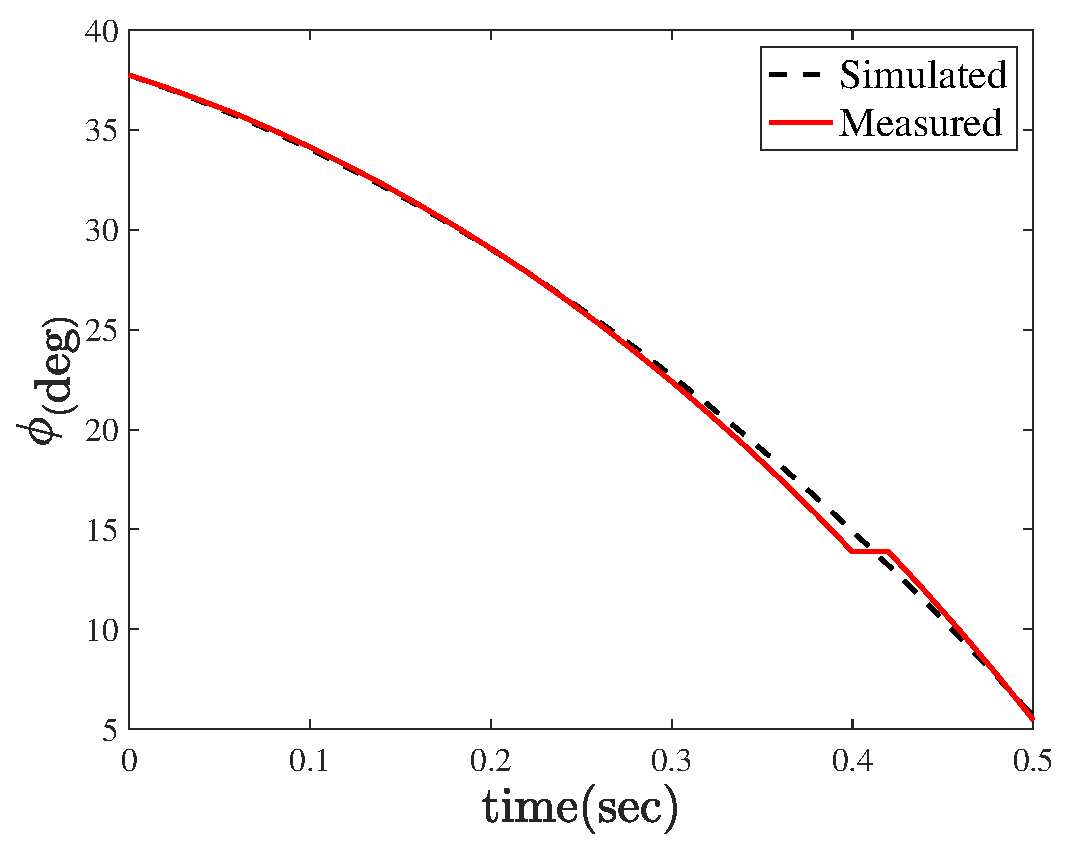
\includegraphics[width=1\linewidth]{../Figure/parameter_estimation/roll/roll}
% 		\captionsetup{justification=centering}
% 		\captionof{figure}{Comparison of roll channel states in simulation and 3DoF setup}
% 	\end{minipage}
% 	\begin{minipage}[b]{0.49\linewidth}
% 		\centering
% 		\begin{tabular}{ccc}\hline
% 			Parameter & Value & Value after evaluation
%             \Tstrut\\ \hline
% 			$\alpha_3$  & $1.1\times10^{-4}$ & $5.47\times10^{-5}$  \Tstrut\\ \hline
% 			\\
% 			\\\\\\\\\\\\\\\\\\
% 		\end{tabular}
% 	\captionsetup{justification=centering}
% 		\captionof{table}{Comparison of roll channel parameter values before and after evaluation}
% 	\end{minipage}
%     \vspace{1cm}
% \end{minipage}

\begin{figure}[H]
	\centering
	\subfloat[]{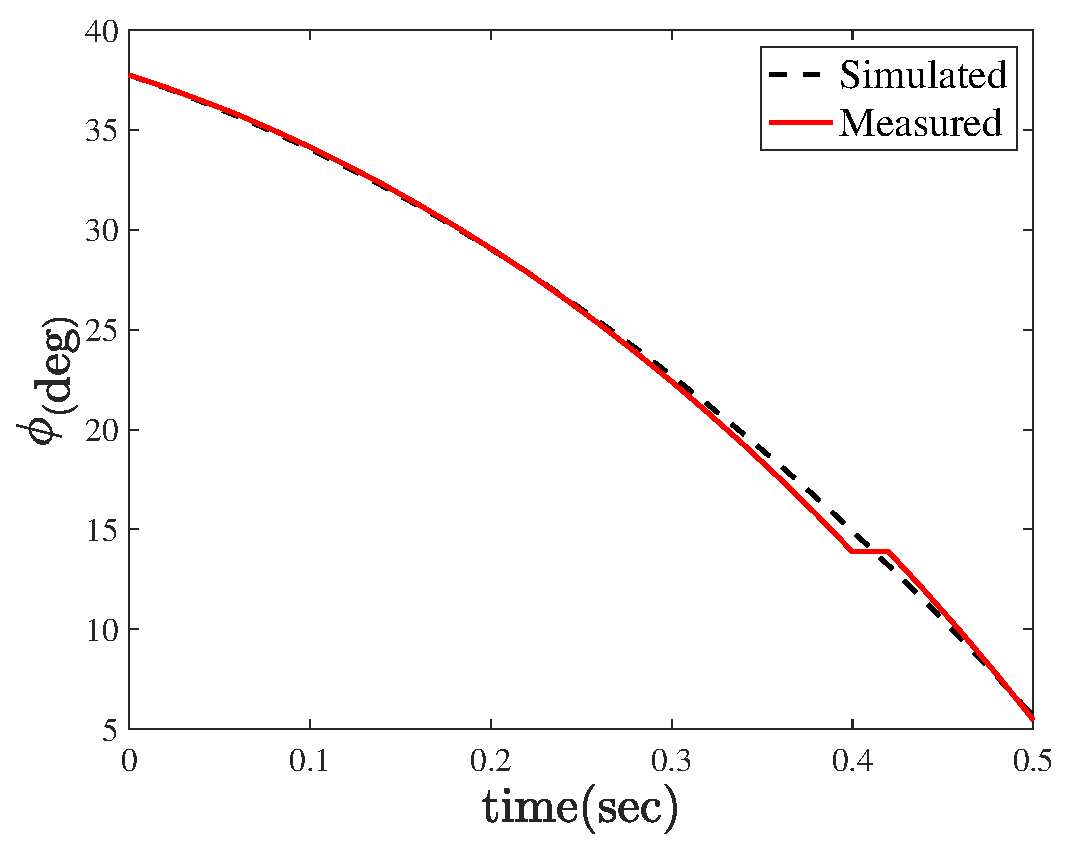
\includegraphics[width=.45\linewidth]{../Figure/parameter_estimation/roll/roll}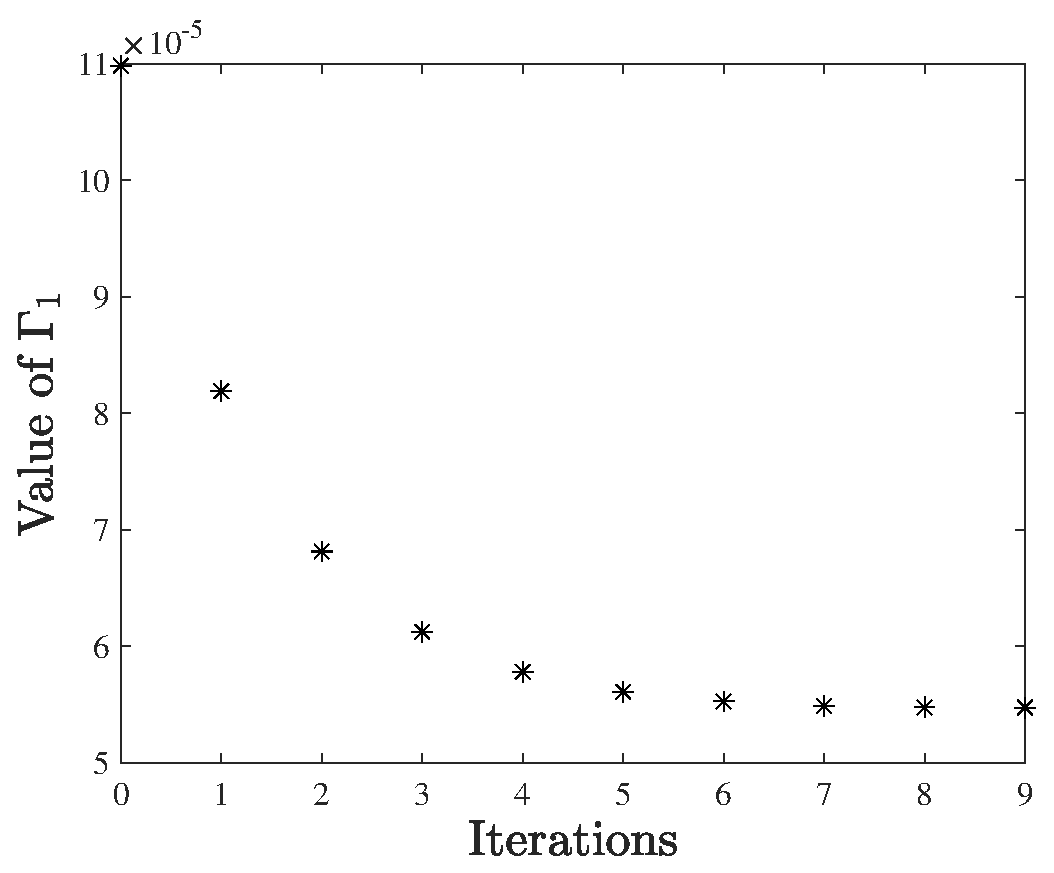
\includegraphics[width=.45\linewidth]{../Figure/parameter_estimation/roll/roll_parameter}
	}
	\hfil
	% \vspace{-0.25cm}
	\subfloat[]{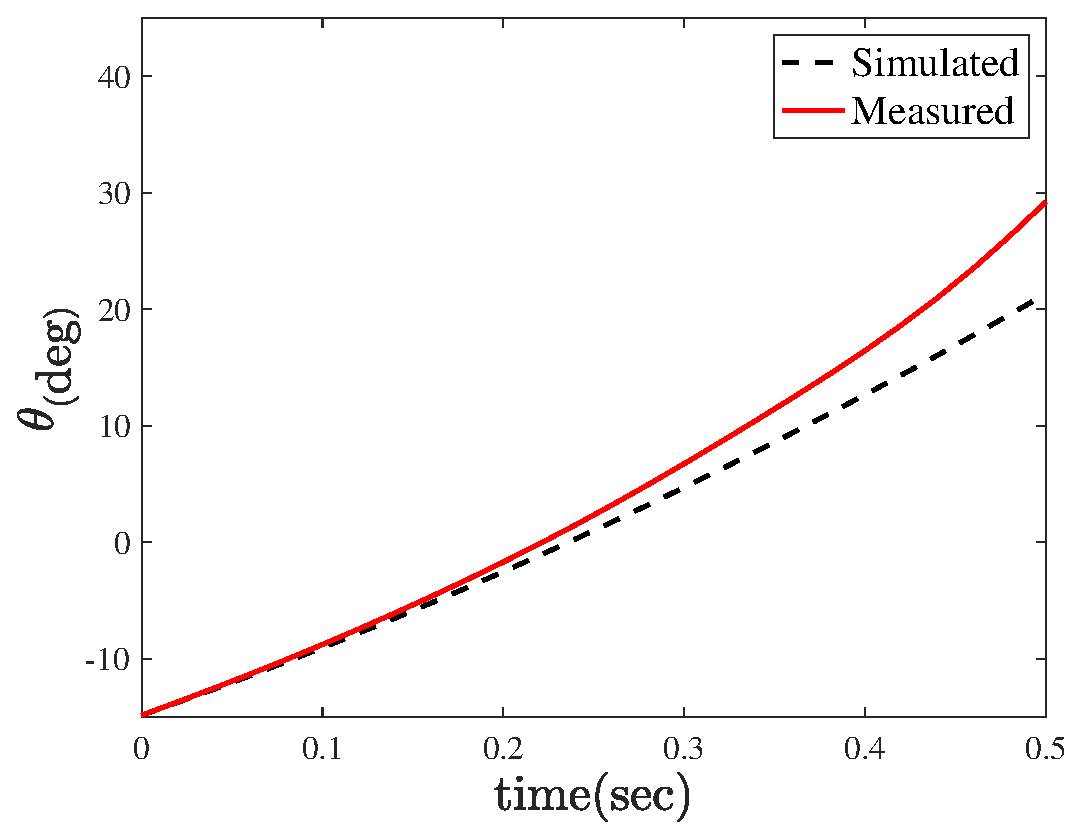
\includegraphics[width=.45\linewidth]{../Figure/parameter_estimation/pitch/pitch}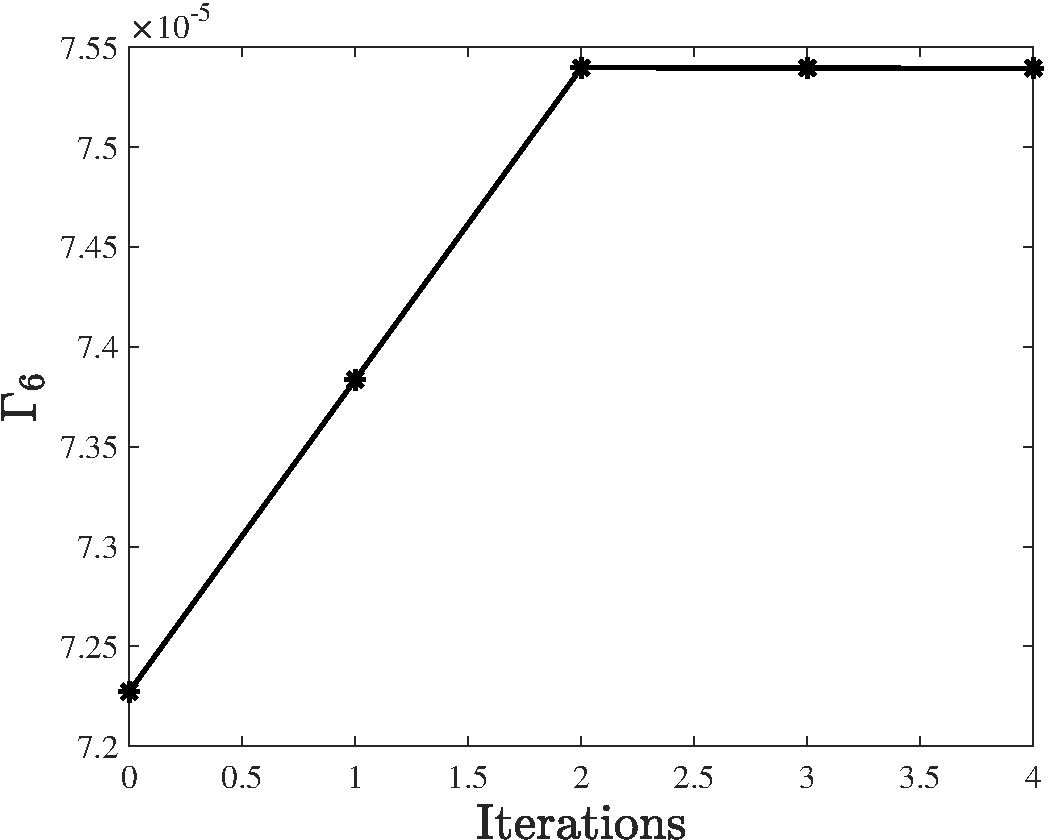
\includegraphics[width=.45\linewidth]{../Figure/parameter_estimation/pitch/pitch_parameter}
	}
	\hfil
	% \vspace{-0.25cm}
	\subfloat[]{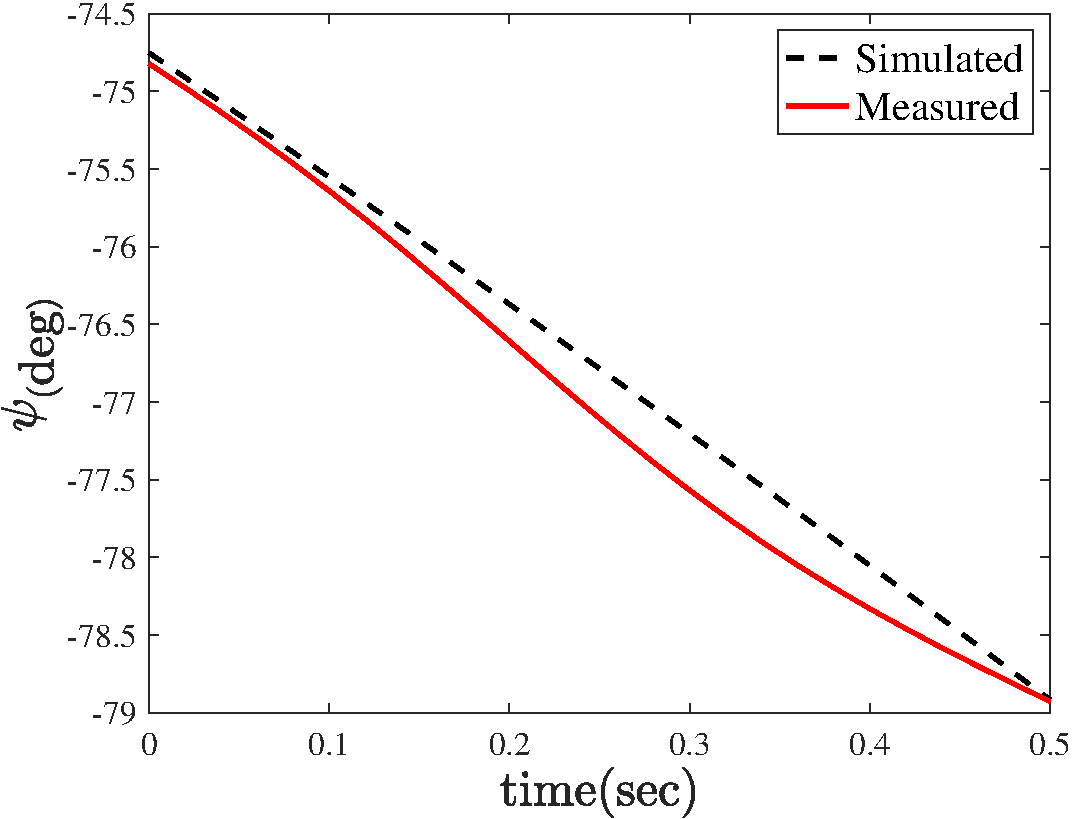
\includegraphics[width=.45\linewidth]{../Figure/parameter_estimation/yaw/yaw}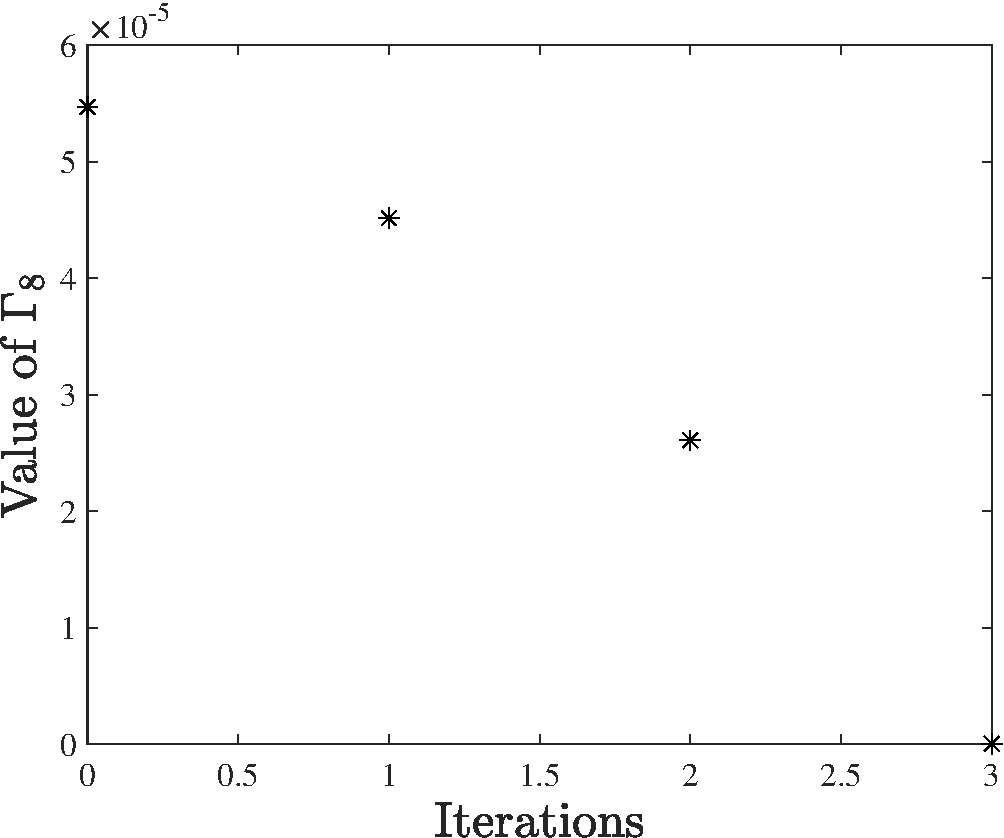
\includegraphics[width=.45\linewidth]{../Figure/parameter_estimation/yaw/yaw_parameter}
	}
	\caption{Identification process results when the quadrotor rotates about only one axis: (a) Identification of $\Gamma_3$ in free roll motion. (b) Identification of $\Gamma_6$ in free pitch motion. (c) Identification of $\Gamma_8$
	in free yaw motion.}
	\label{fig:one_degree_identification}
\end{figure}


\begin{figure}[H]
	\centering
	\subfloat[]{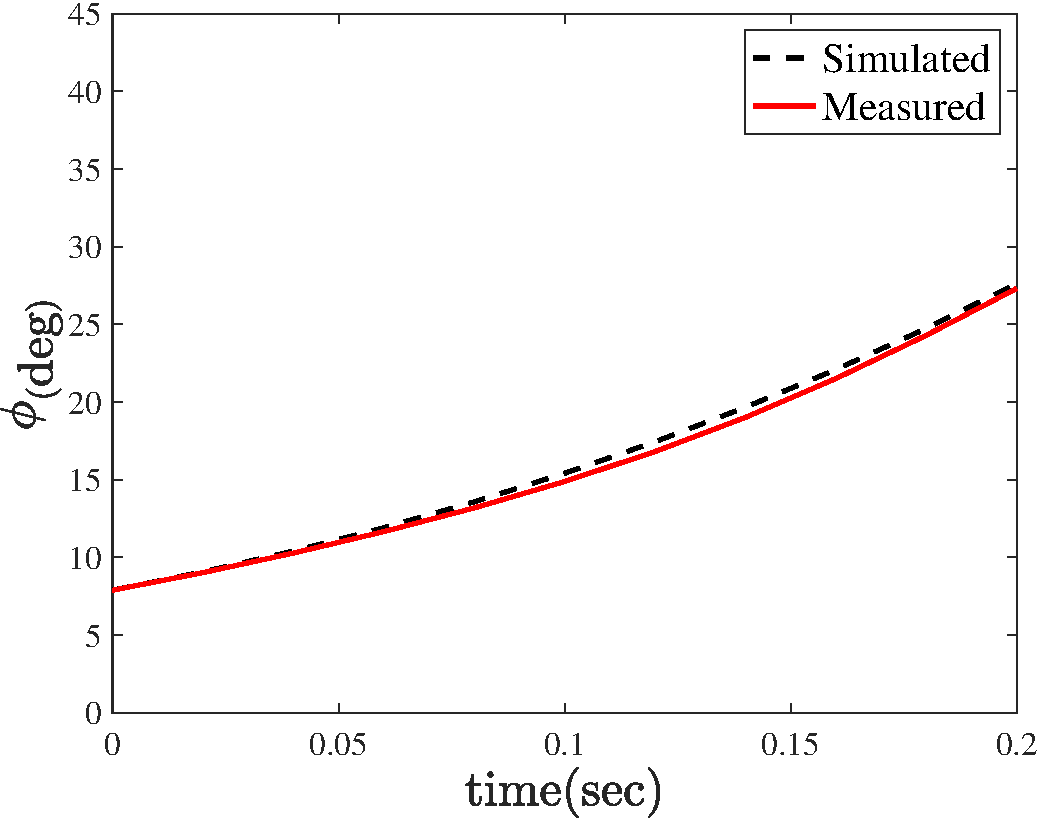
\includegraphics[width=.45\linewidth]{../Figure/parameter_estimation/roll-pitch/roll}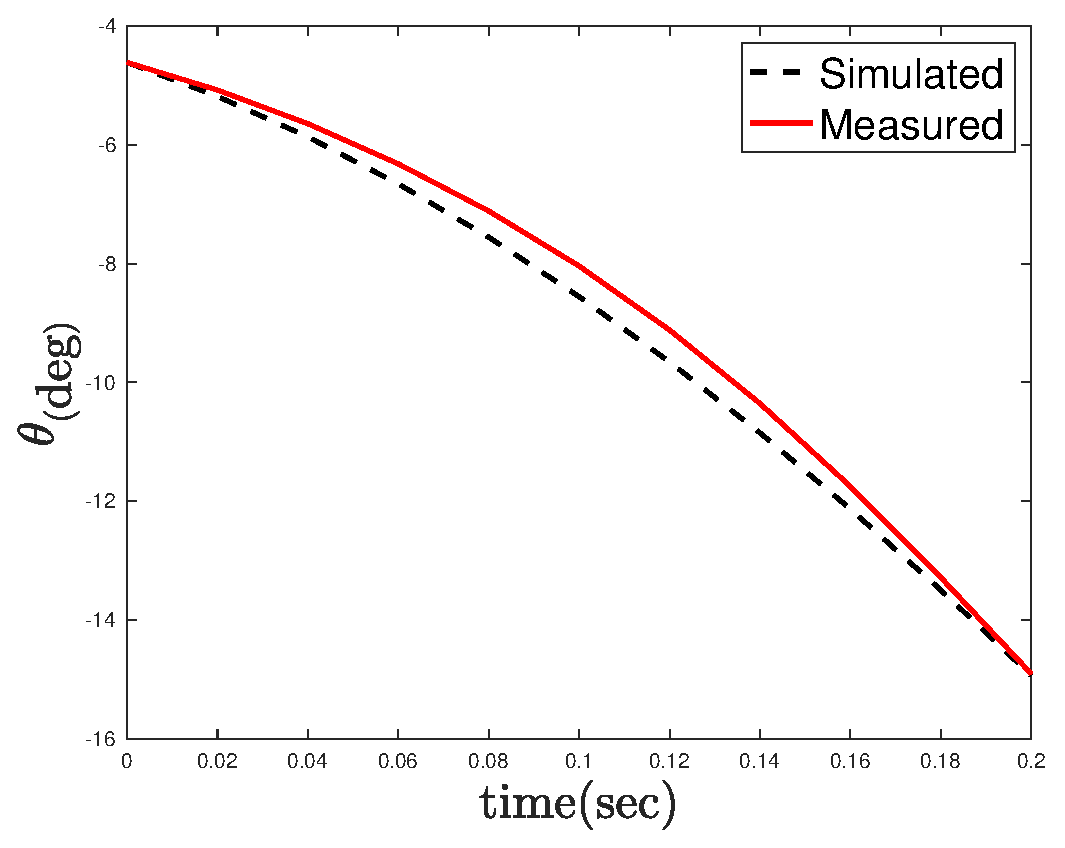
\includegraphics[width=.45\linewidth]{../Figure/parameter_estimation/roll-pitch/pitch}
	}
	\hfil
	% \vspace{-0.25cm}
	\subfloat[]{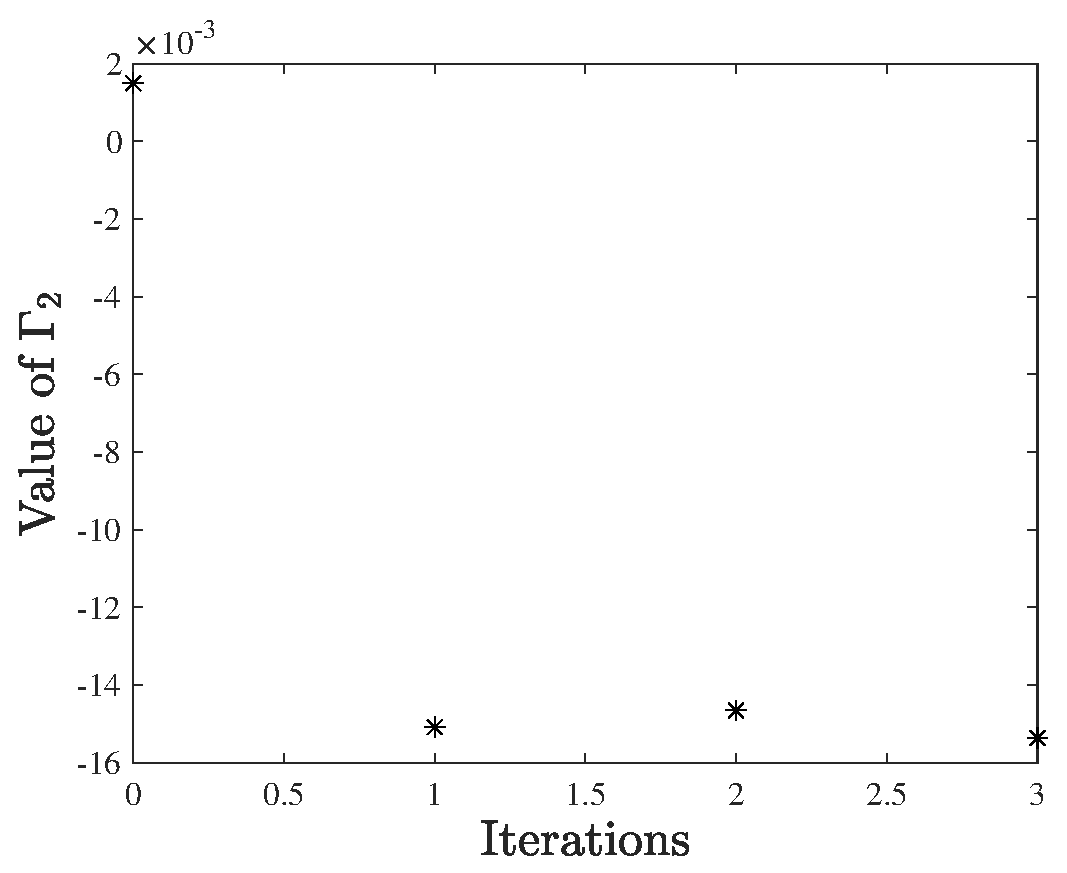
\includegraphics[width=.45\linewidth]{../Figure/parameter_estimation/roll-pitch/roll_parameter}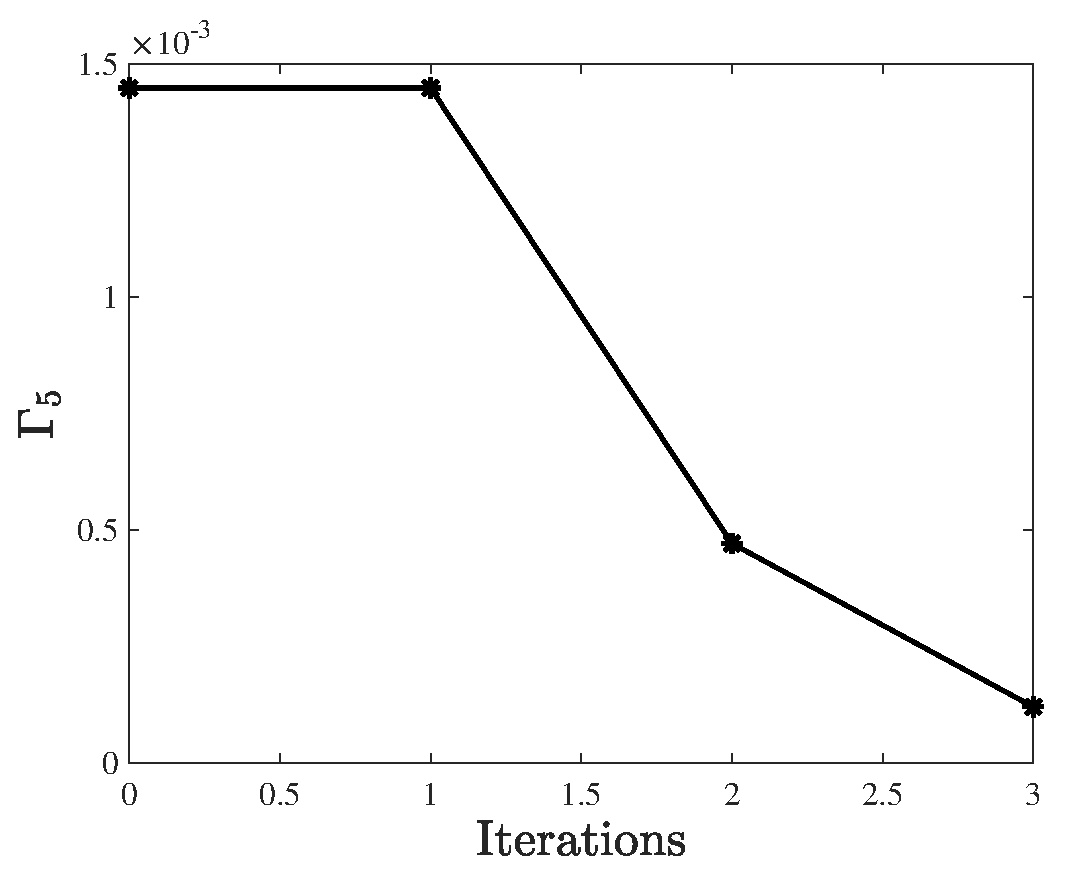
\includegraphics[width=.45\linewidth]{../Figure/parameter_estimation/roll-pitch/pitch_parameter}
	}
	\caption{Identification process results when the quadrotor rotates about its roll and pitch axes:
	(a) Comparison of Simulation and experimental results. (b) Identification of $\Gamma_2$ and $\Gamma_5$.}
	\label{fig:two_degree_identification}
\end{figure}



\begin{figure}[H]
	\centering
	\subfloat[]{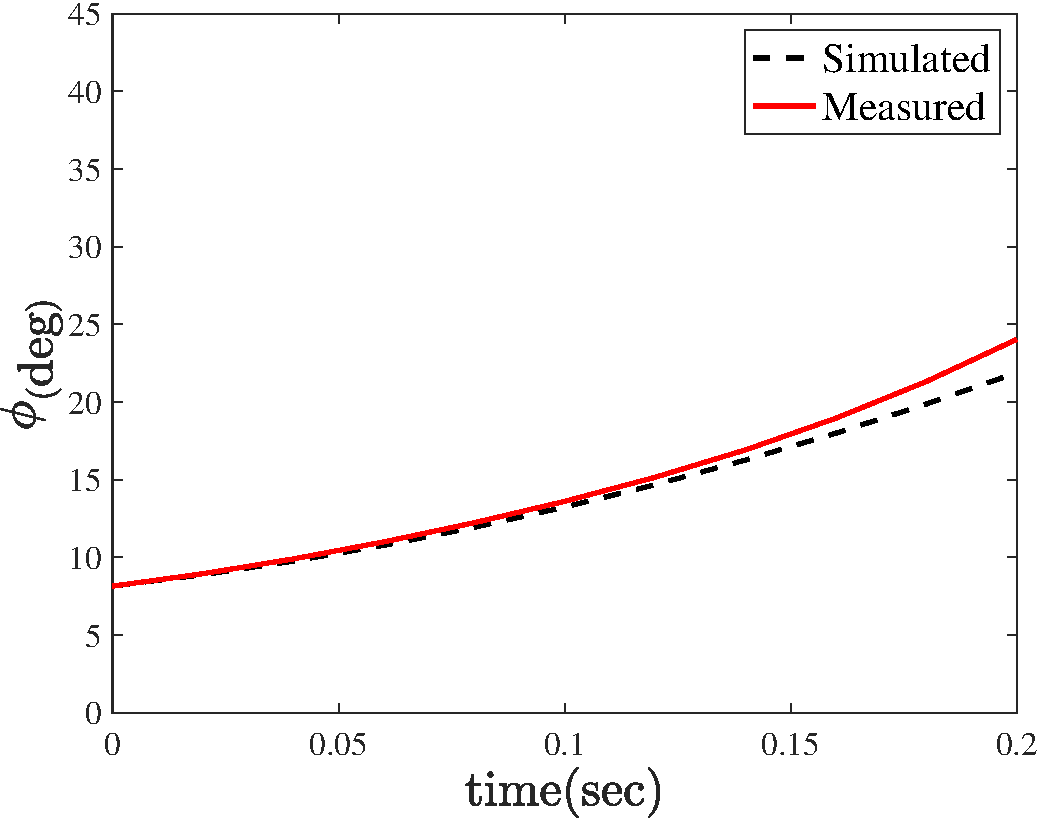
\includegraphics[width=.33\linewidth]{../Figure/parameter_estimation/3DOF/roll}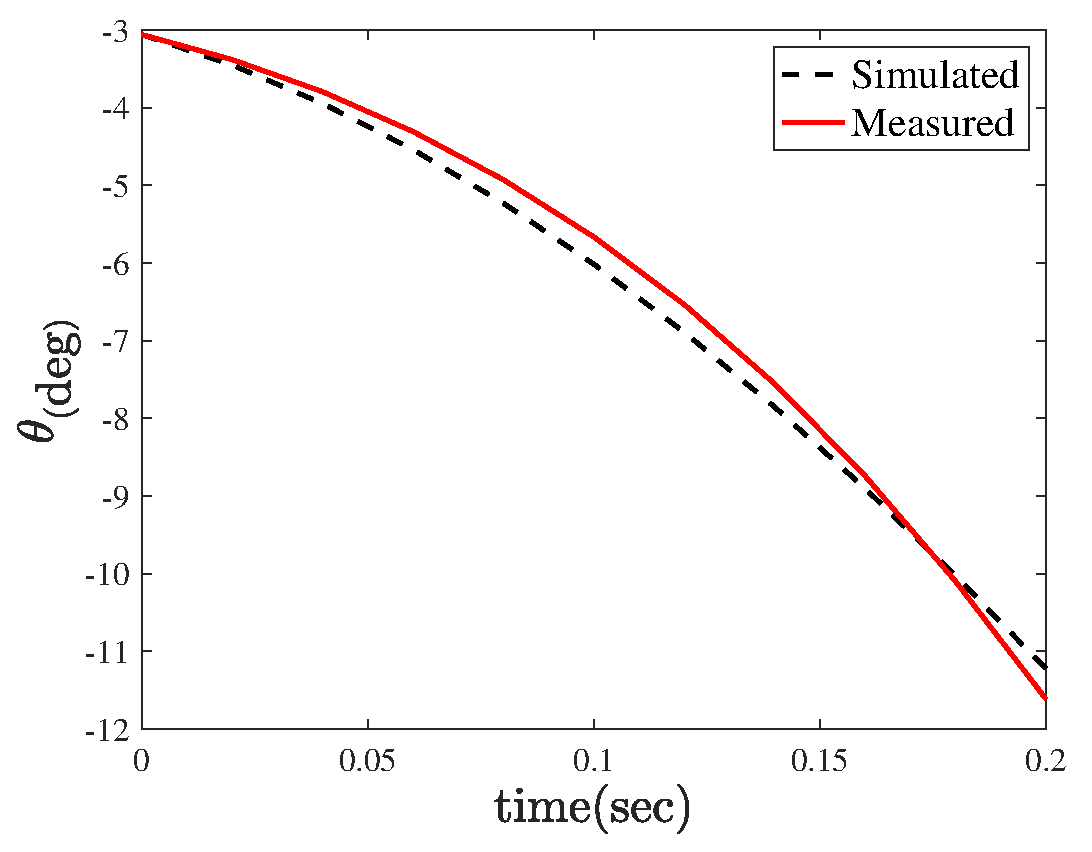
\includegraphics[width=.33\linewidth]{../Figure/parameter_estimation/3DOF/pitch}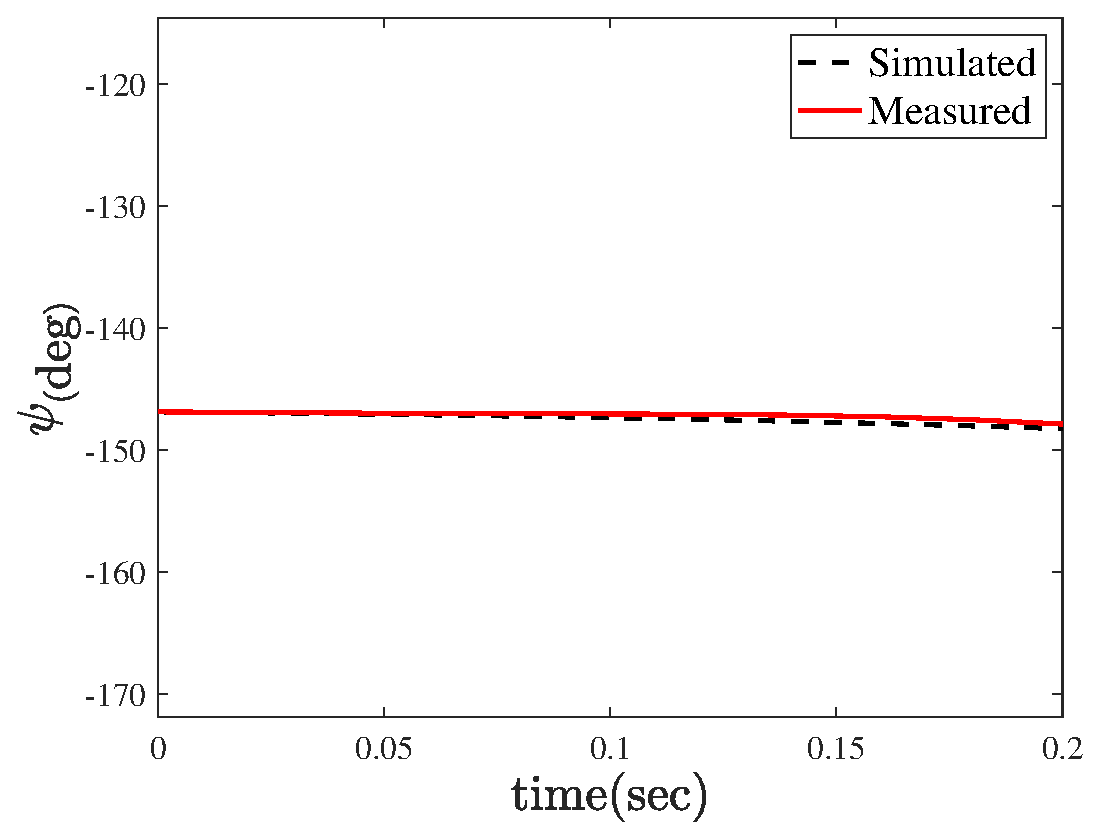
\includegraphics[width=.33\linewidth]{../Figure/parameter_estimation/3DOF/yaw}
	}
	\hfil
	\subfloat[]{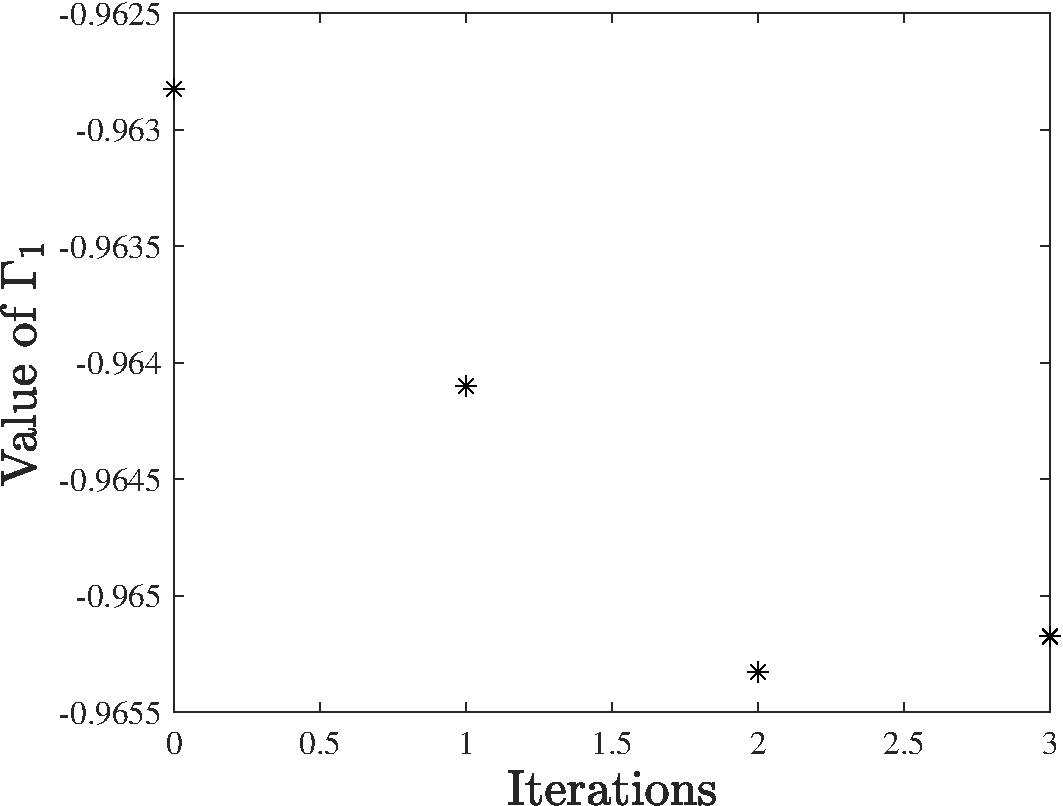
\includegraphics[width=.33\linewidth]{../Figure/parameter_estimation/3DOF/roll_parameter}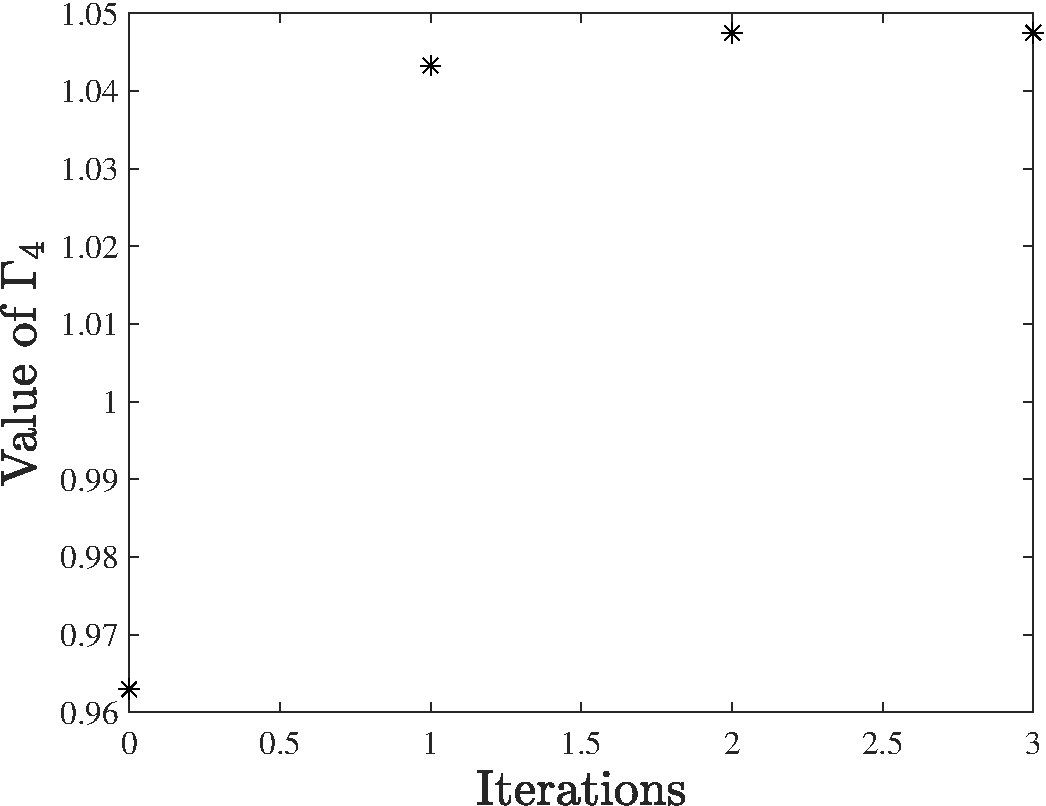
\includegraphics[width=.33\linewidth]{../Figure/parameter_estimation/3DOF/pitch_parameter}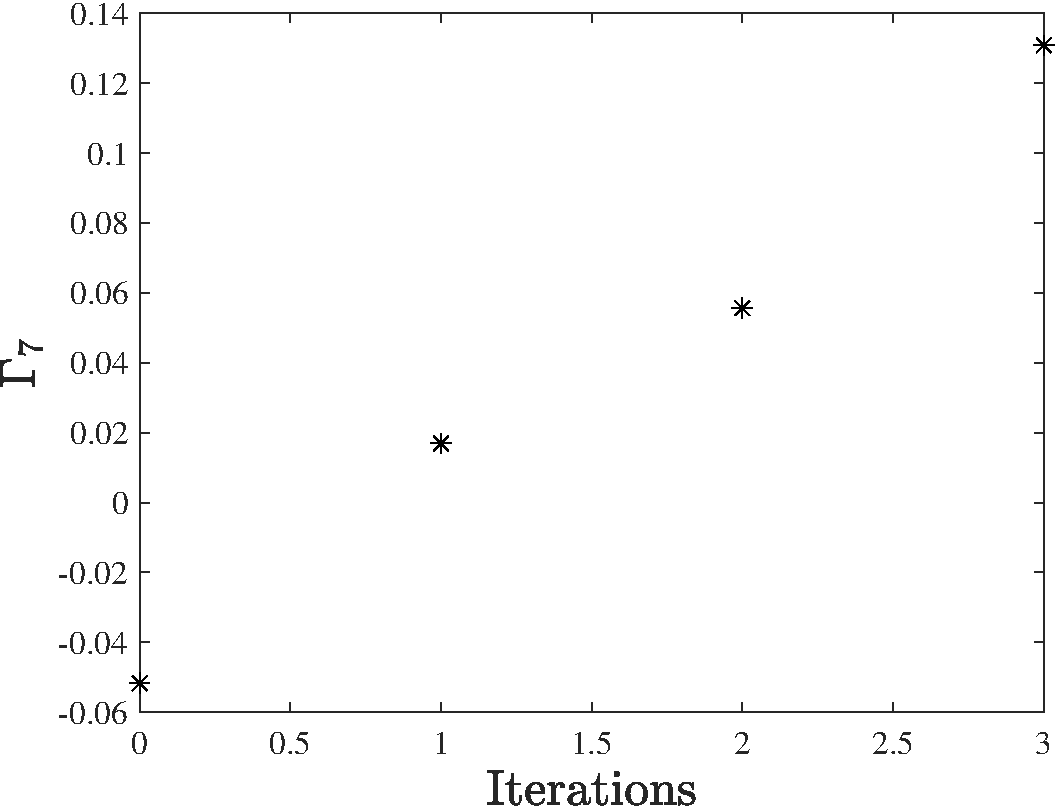
\includegraphics[width=.33\linewidth]{../Figure/parameter_estimation/3DOF/yaw_parameter}
	}
	\caption{Identification process results when the quadrotor rotates about its roll, pitch, and yaw axes: (a) Comparison of Simulation and experimental results. (b) Identification of $\Gamma_1$ , $\Gamma_4$ and
	$\Gamma_7$ parameters.}
	\label{fig:three_degree_identification}
\end{figure}




% \begin{minipage}[t]{0.95\linewidth}
% 	\hfill
%     \begin{minipage}[b]{0.48\linewidth}
% 		\centering
% 		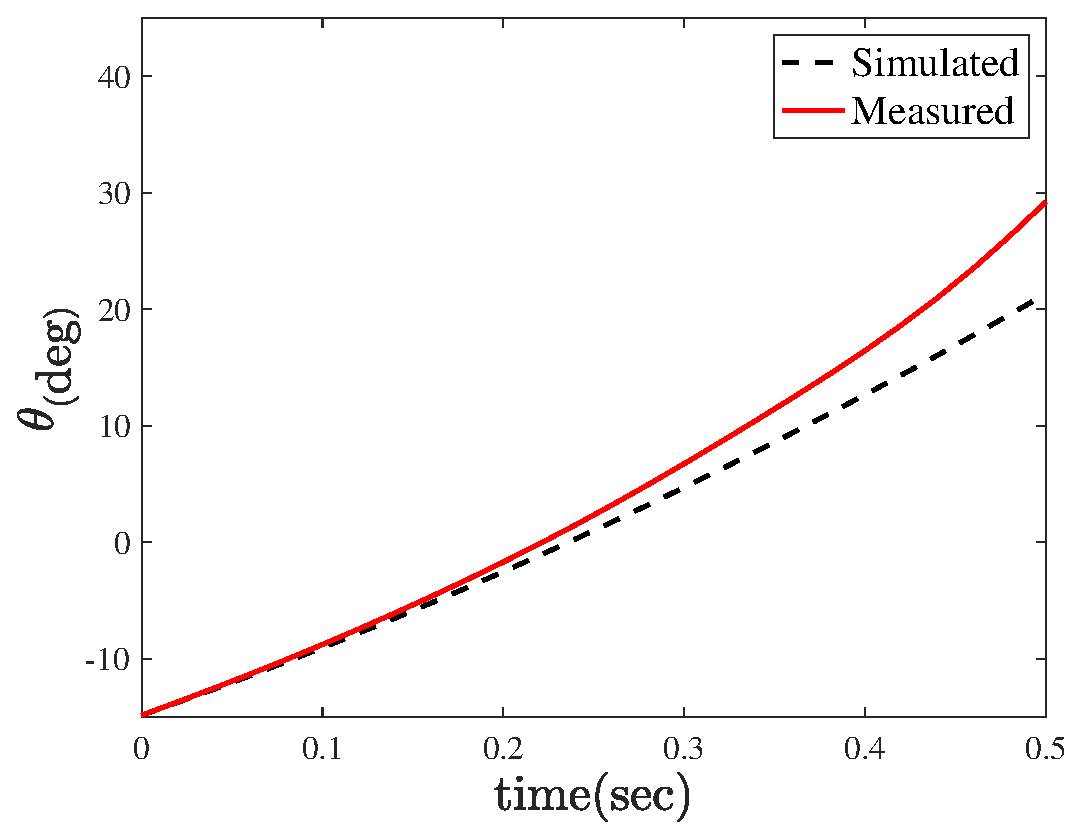
\includegraphics[width=1\linewidth]{../Figure/parameter_estimation/pitch/pitch}
% 		\captionsetup{justification=centering}
% 		\captionof{figure}{Comparison of pitch channel states in simulation and 3DoF setup}
% 	\end{minipage}
% 	\begin{minipage}[b]{0.49\linewidth}
% 		\centering
% 		\begin{tabular}{ccc}\hline
% 			Parameter & Value & Value after evaluation
%             \Tstrut\\ \hline
% 			$\beta_3$  & $1.1\times10^{-4}$ & $7.13\times10^{-5}$  \Tstrut\\ \hline
% 			\\
% 			\\\\\\\\\\\\\\\\\\
% 		\end{tabular}
% 	\captionsetup{justification=centering}
% 		\captionof{table}{Comparison of pitch channel parameter values before and after evaluation}
% 	\end{minipage}
% \end{minipage}

% % \vspace{1cm}

% \begin{minipage}[t]{0.95\linewidth}
% 	\hfill
%     \begin{minipage}[b]{0.48\linewidth}
% 		\centering
% 		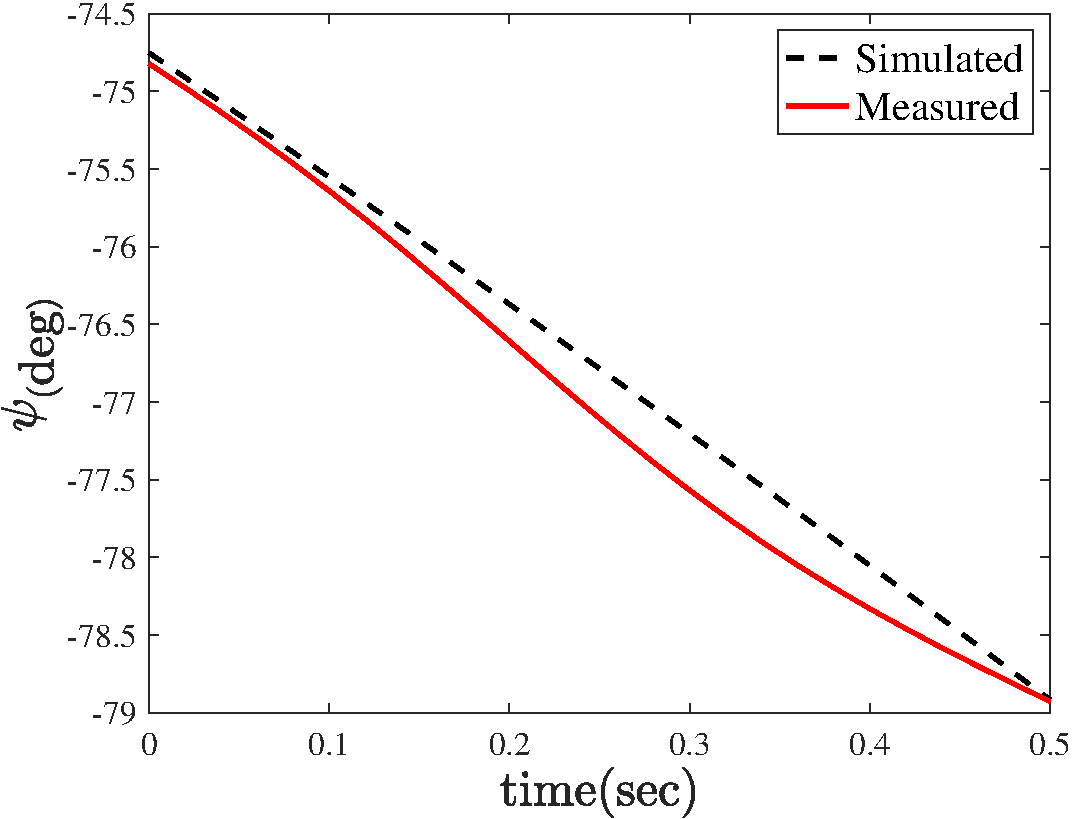
\includegraphics[width=1\linewidth]{../Figure/parameter_estimation/yaw/yaw}
% 		\captionsetup{justification=centering}
% 		\captionof{figure}{Comparison of yaw channel states in simulation and 3DoF setup}
% 	\end{minipage}
% 	\begin{minipage}[b]{0.49\linewidth}
% 		\centering
% 		\begin{tabular}{ccc}\hline
% 			Parameter & Value & Value after evaluation
%             \Tstrut\\ \hline
% 			$\gamma_2$  & $5.5\times10^{-5}$ & $1.3\times10^{-6}$  \Tstrut\\ \hline
% 			\\
% 			\\\\\\\\\\\\\\\\\\
% 		\end{tabular}
% 	\captionsetup{justification=centering}
% 		\captionof{table}{Comparison of yaw channel parameter values before and after evaluation}
% 	\end{minipage}
% \end{minipage}

% \begin{minipage}[t]{0.95\linewidth}
% 	\hfill
%     \begin{minipage}[b]{0.48\linewidth}
% 		\centering
% 		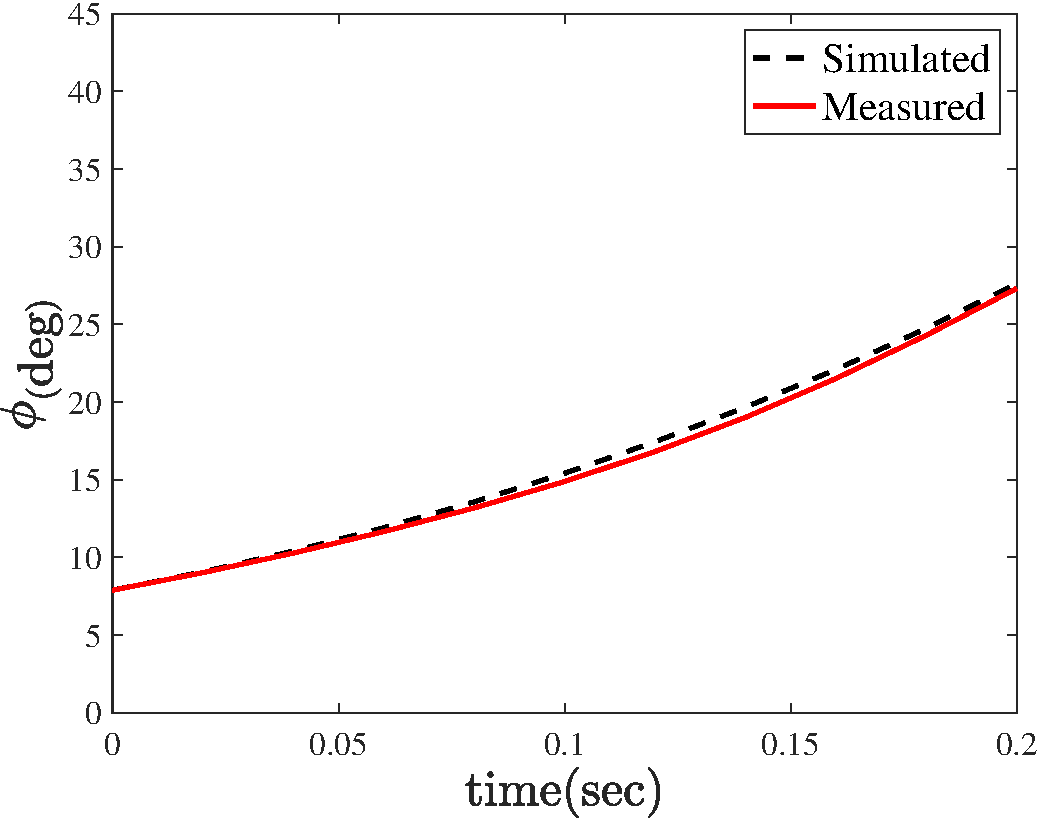
\includegraphics[width=1\linewidth]{../Figure/parameter_estimation/roll-pitch/roll}
% 		\captionsetup{justification=centering}
% 		\captionof{figure}{Comparison of roll channel states in simulation and 3DoF setup}
% 	\end{minipage}
%     \begin{minipage}[b]{0.48\linewidth}
% 		\centering
% 		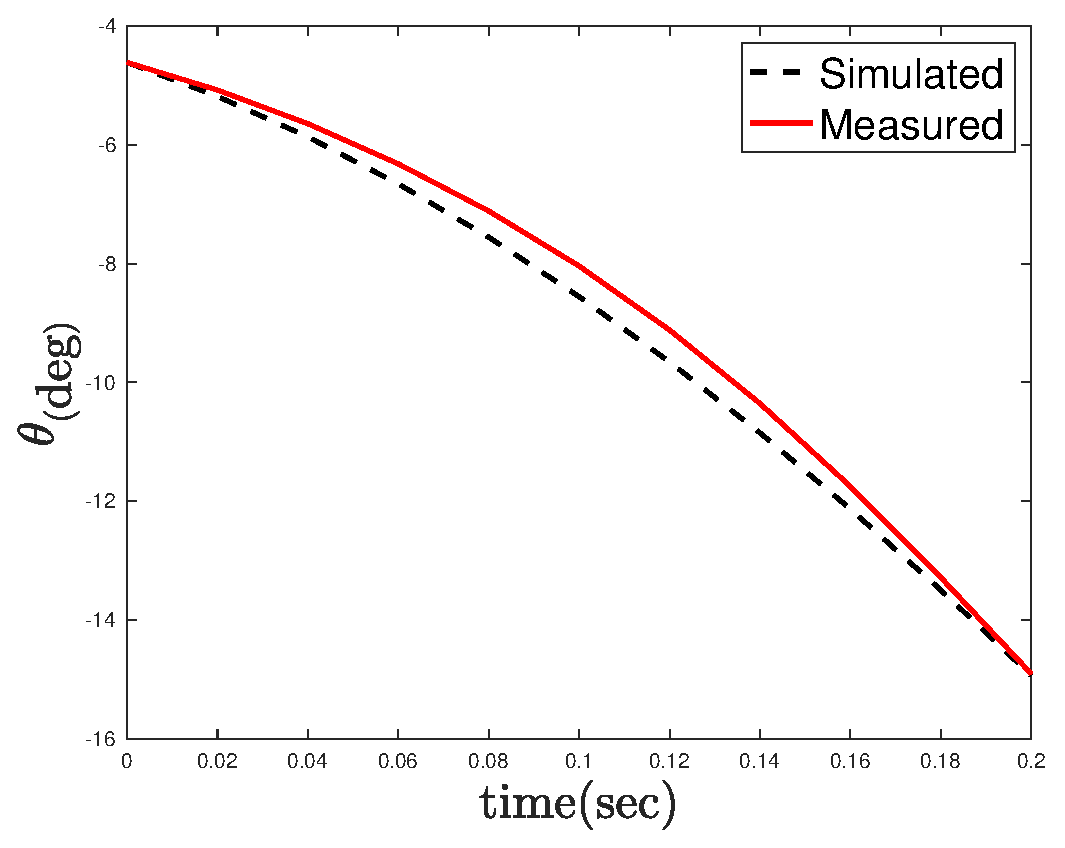
\includegraphics[width=1\linewidth]{../Figure/parameter_estimation/roll-pitch/pitch}
% 		\captionsetup{justification=centering}
% 		\captionof{figure}{Comparison of pitch channel states in simulation and 3DoF setup}
% 	\end{minipage}
%     \hfill
%     \begin{minipage}[b]{1\linewidth}
% 		\centering
% 		\begin{tabular}{ccc}\hline
% 			Parameter & Value & Value after evaluation
%             \Tstrut\\ \hline
% 			$\alpha_2$  & 0.0015 & 0.0020\Tstrut\\
%             $\beta_2$  & 0.0015 & 0.0027\Tstrut\\ \hline
% 		\end{tabular}
% 	\captionsetup{justification=centering}
% 		\captionof{table}{Comparison of roll-pitch channel parameter values before and after evaluation}
% 	\end{minipage}
% \end{minipage}


%     \begin{minipage}[b]{0.48\linewidth}
% 		\centering
% 		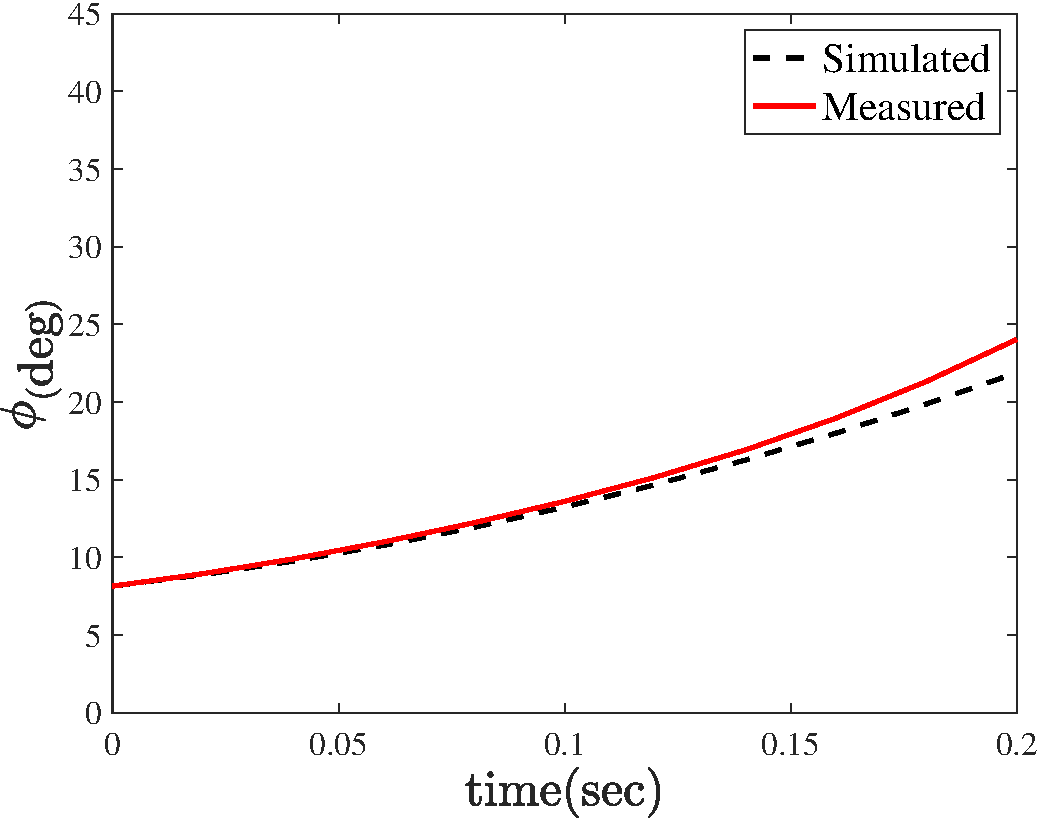
\includegraphics[width=1\linewidth]{../Figure/parameter_estimation/3DOF/roll}
% 		\captionsetup{justification=centering}
% 		\captionof{figure}{Comparison of roll channel states in simulation and 3DoF setup}
% 	\end{minipage}
%     \begin{minipage}[b]{0.48\linewidth}
% 		\centering
% 		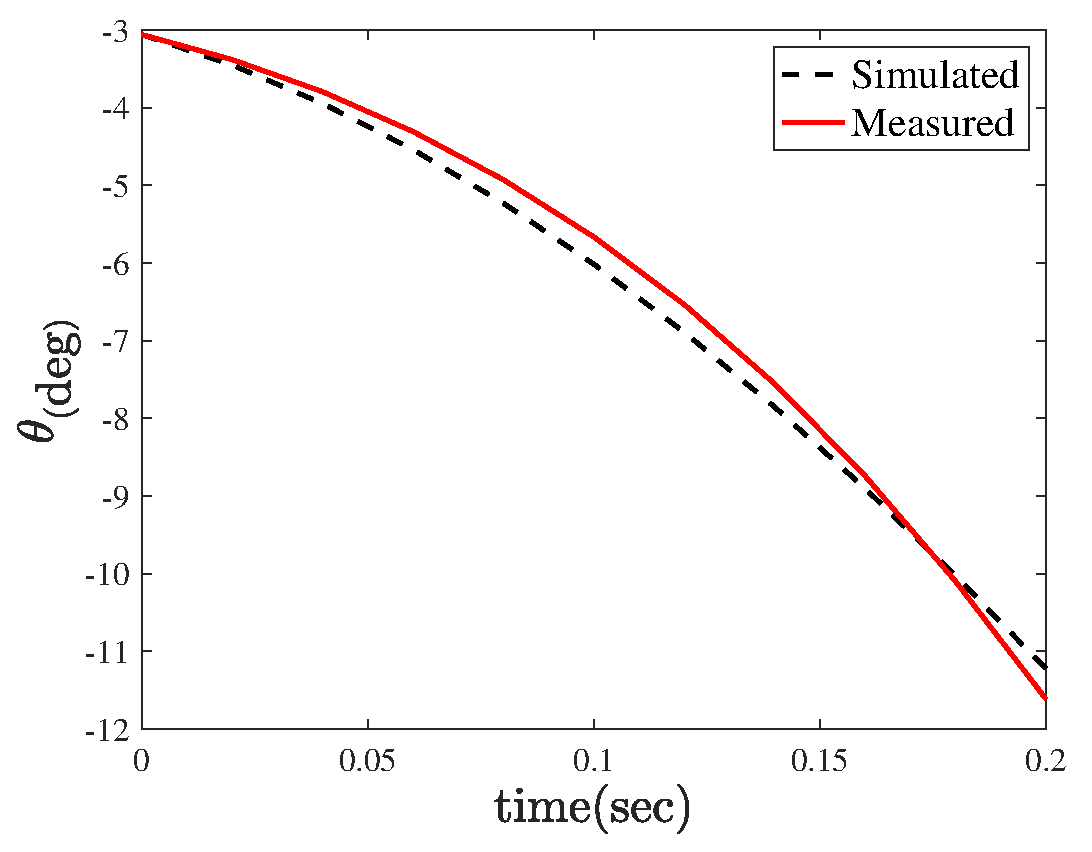
\includegraphics[width=1\linewidth]{../Figure/parameter_estimation/3DOF/pitch}
% 		\captionsetup{justification=centering}
% 		\captionof{figure}{Comparison of pitch channel states in simulation and 3DoF setup}
% 	\end{minipage}
%     \hfill
%     \begin{minipage}[b]{0.48\linewidth}
% 		\centering
% 		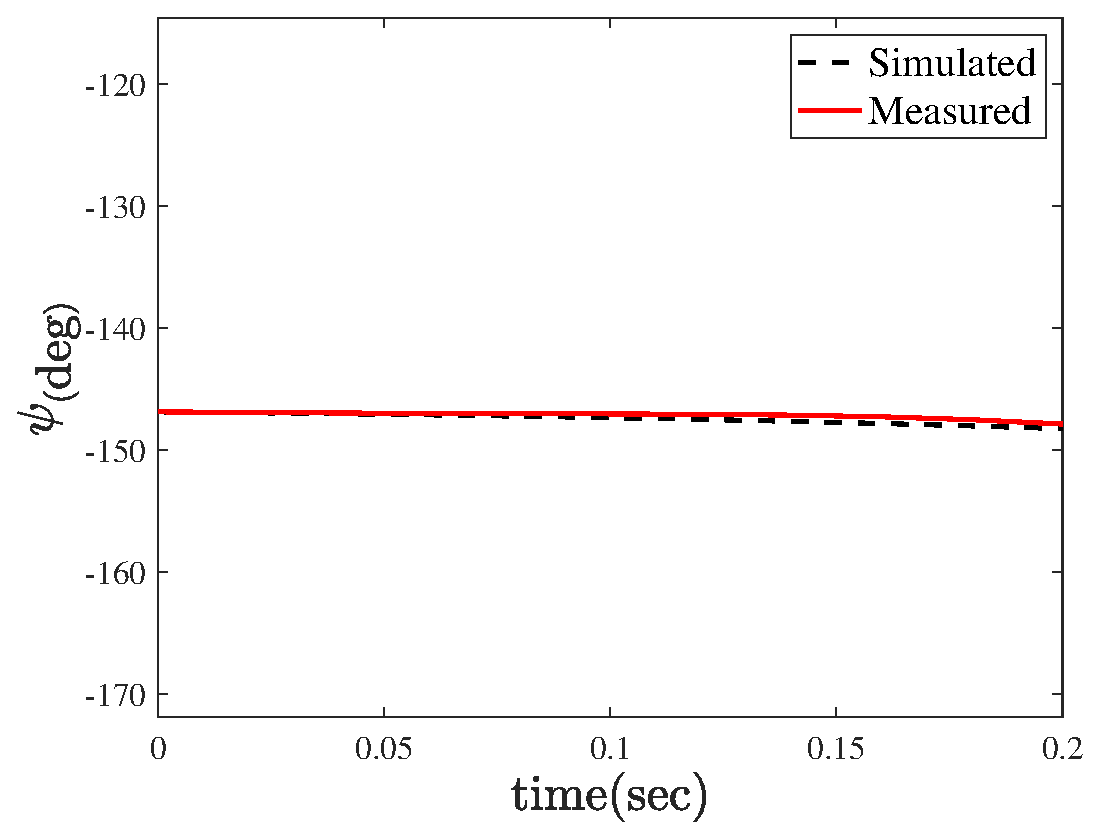
\includegraphics[width=1\linewidth]{../Figure/parameter_estimation/3DOF/yaw}
% 		\captionsetup{justification=centering}
% 		\captionof{figure}{Comparison of yaw channel states in simulation and 3DoF setup}
% 	\end{minipage}
%     \begin{minipage}[b]{0.48\linewidth}
% 		\centering
% 		\begin{tabular}{ccc}\hline
% 			Parameter & Value & Value after evaluation
%             \Tstrut\\ \hline
% 			$\alpha_1$  & -0.9628 & -1.56\Tstrut\\
%             $\beta_1$  & 0.9629 & 1.57\Tstrut \\
%             $\gamma_1$  & -0.0017 &-0.085\Tstrut\\ \hline
%             \\\\\\\\\\\\\\\\
% 		\end{tabular}
% 	\captionsetup{justification=centering}
% 		\captionof{table}{Comparison of 3DOF channel parameter values before and after evaluation}
% 	\end{minipage}


\subsection{Evaluation of LQIR-DG Performance}
% \noindent Here, the performance of the LQIR-DG controller is evaluated. The desired and actual outputs, including the roll, pitch, and yaw angles, are compared in figure \ref{fig:result}. The desired scenario of the simulator is considered a level flight. These figures show that the attitude outputs of the quadrotor converge to the desired values in less than three seconds. Moreover, figure \ref{fig:omega} shows the angular velocity command of the quadrotor, 
% respectively. These results illustrate that the LQIR-DG approach appropriately controls the attitude of the experimental setup of the quadrotor.

% The performance of the LQIR-DG control strategy is assessed in three aspects: regulation and following of a square wave reference signal, disturbance rejection, and model uncertainty. The regulation and following of the square wave reference signal are examined in Section \ref{sec:regulation}. The effectiveness of the controller in rejecting different levels of disturbance is evaluated in Section \ref{sec:disturbance}. Moreover, the impact of model uncertainty on the performance of the controller is studied in Section \ref{sec:model-uncertainty}.

\noindent Here, the performance of the LQIR-DG controller algorithm is evaluated for regulation and tracking performance, disturbance rejection, and the impact of model uncertainty.
% \noindent Here, the performance of the LQIR-DG controller is evaluated using algorithms for regulation and tracking performance, disturbance rejection, and the impact of model uncertainty.
Finally, the performance of the proposed controller is compared to the PID controller and variants of the LQR controller. The parameters of the PID controller are presented in Table \ref{tab:PID_parameters}.

% \begin{table}[H]
% 	\renewcommand{\arraystretch}{1.3}
% 	\caption{Parameters of PID Controller}
% 	\begin{center}
% 	\begin{tabular}{c |c c c}
% 	\cmidrule{2-4}
% 	 & \textbf{\textit{p}}& \textbf{i} & \textbf{\textit{d}}  \\
% 	\hline
% 	$\Gamma_1$ & $-0.9622$ & $\Gamma_5$ & $3.6441\times10^{-4}$ \\

% 	$\Gamma_2$ & $-0.0154$ & $\Gamma_6$ & $7.5395\times10^{-5}$ \\

% 	$\Gamma_3$ &$5.4716\times10^{-5}$ & $\Gamma_7$ & $0.1308$ \\

% 	$\Gamma_4$ & $1.0457$ & $\Gamma_8$ & $4.3753\times10^{-5}$ \\
% 	\hline
% 	\end{tabular}
% 	\label{tab:PID_parameters}
% 	\end{center}
% \end{table}


\begin{table}[H]
	\renewcommand{\arraystretch}{1.3}
	\caption{Parameters of PID Controller}
	\begin{center}
		\begin{tabular}{cccc}
		\hline
		\textbf{Channel} & \textbf{$K_p$} & \textbf{$K_i$} & \textbf{$K_d$} \\
		\hline
		Roll & 2.0 & 0.5 & 1.0 \\
		Pitch & 1.5 & 0.4 & 0.8 \\
		Yaw & 3.0 & 0.6 & 1.2 \\
		\hline
		\end{tabular}
		\label{tab:PID_parameters}
	\end{center}
\end{table}

% \begin{table}[H]{\arraystretch}{1.3}
% 	\centering
% 	\caption{PID Controller Parameters for Three Systems}
% 	\begin{tabular}{cccc}
% 	\hline
% 	\textbf{Channel} & \textbf{$K_p$} & \textbf{$K_i$} & \textbf{$K_d$} \\
% 	\hline
% 	Roll & 2.0 & 0.5 & 1.0 \\
% 	Pitch & 1.5 & 0.4 & 0.8 \\
% 	Yaw & 3.0 & 0.6 & 1.2 \\
% 	\hline
% 	\end{tabular}
% 	\label{tab:pid-parameters}
% \end{table}



\subsubsection{Performance of the LQIR-DG Controller}\label{sec:regulation}
% \noindent This experiment assesses the efficacy of the LQIR-DG controller in regulating and following a square wave input for the quadrotor's attitude angles. The desired square wave input is generated for the roll and pitch angles, and the quadrotor's response to the input is measured. The results obtained demonstrate the robustness and precision of the LQIR-DG controller in accurately tracking the square wave input.
\noindent Here, the results of the LQIR-DG controller method are presented for the control loops of the Euler angles of the experimental platform in Figures \ref{fig:result} and \ref{fig:omega}.
The performance of the proposed controller is evaluated in Figure \ref{fig:result}.
Figure \ref{fig:result} \ref{sub@fig:regulation} compares the desired and output signals, i.e., the Euler angles during regulation. Figure \ref{fig:result} \ref{sub@fig:square} compares the desired square wave input with a frequency of 0.02 Hz and an amplitude of 20 degrees with the output signals in the two-degree-of-freedom coupling mode.

Moreover, Figures \ref{fig:omega} \ref{sub@fig:omega_regulation} and \ref{sub@fig:omega_square} show the rotational velocity command of the quadrotor in the regulation and tracking problems, respectively. These results demonstrate that the roll, pitch, and yaw angles are accurately controlled by the proposed approach.


\begin{figure}[H]
	\centering
	\subfloat[\label{fig:regulation}]{{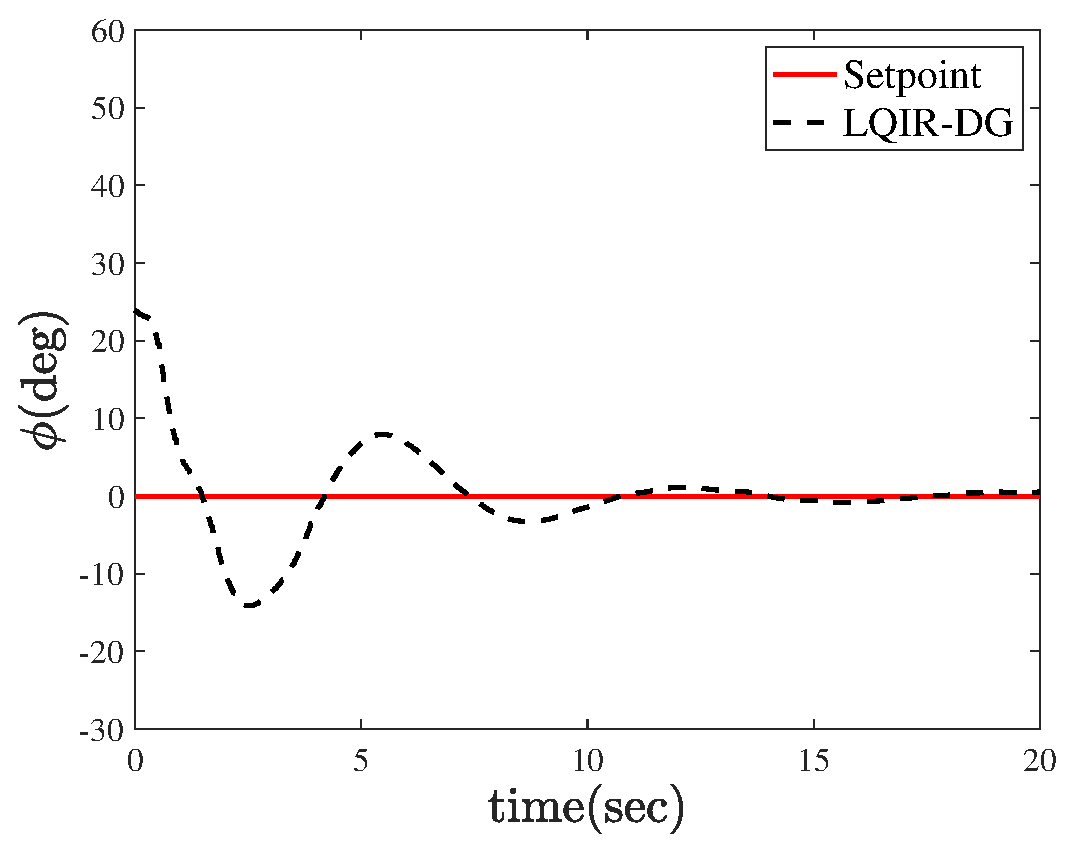
\includegraphics[width=.3\linewidth]{../Figure/implementation/lqidg_roll}}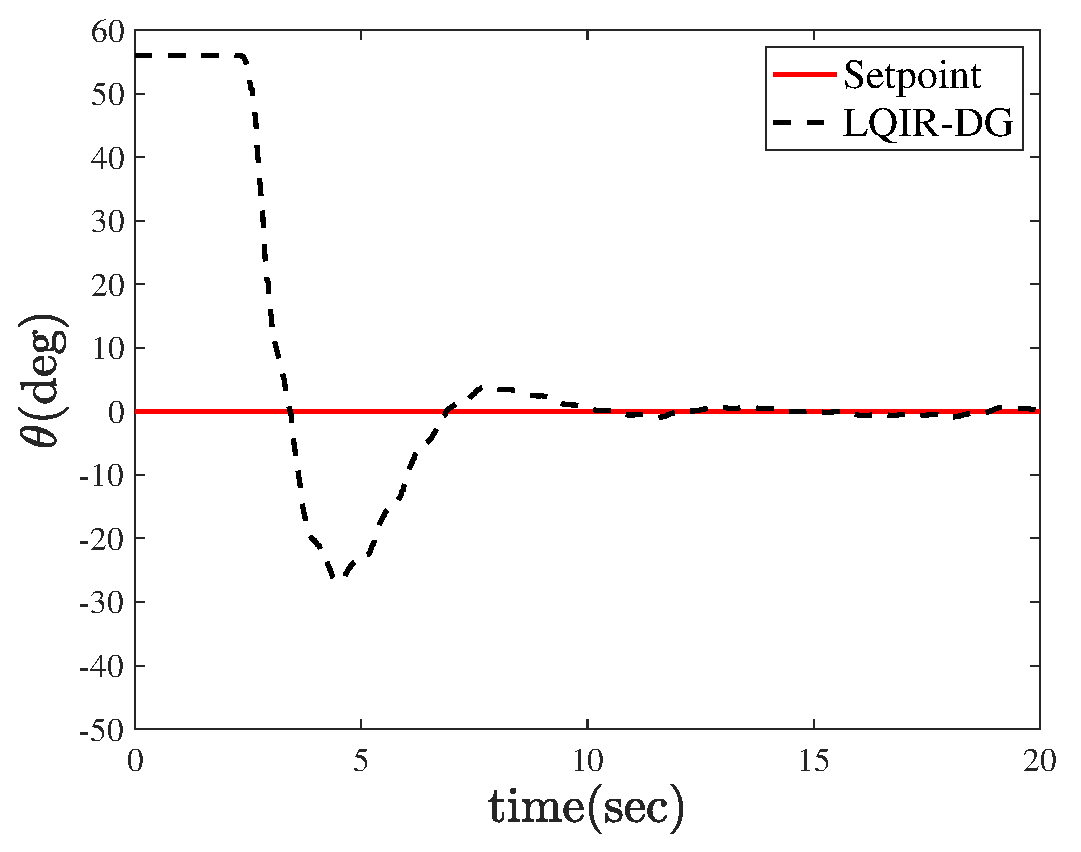
\includegraphics[width=.3\linewidth]{../Figure/implementation/lqidg_pitch}
	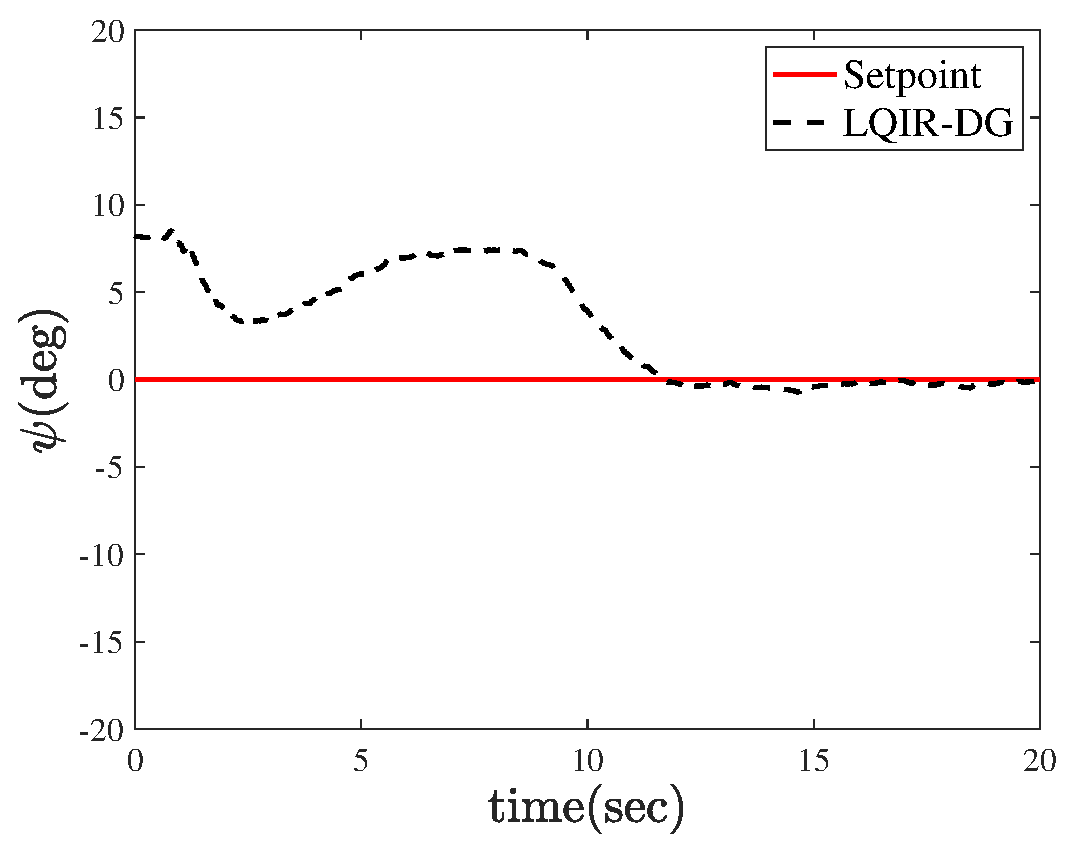
\includegraphics[width=.3\linewidth]{../Figure/implementation/lqidg_yaw}}
	\hfill
	\subfloat[\label{fig:square}]{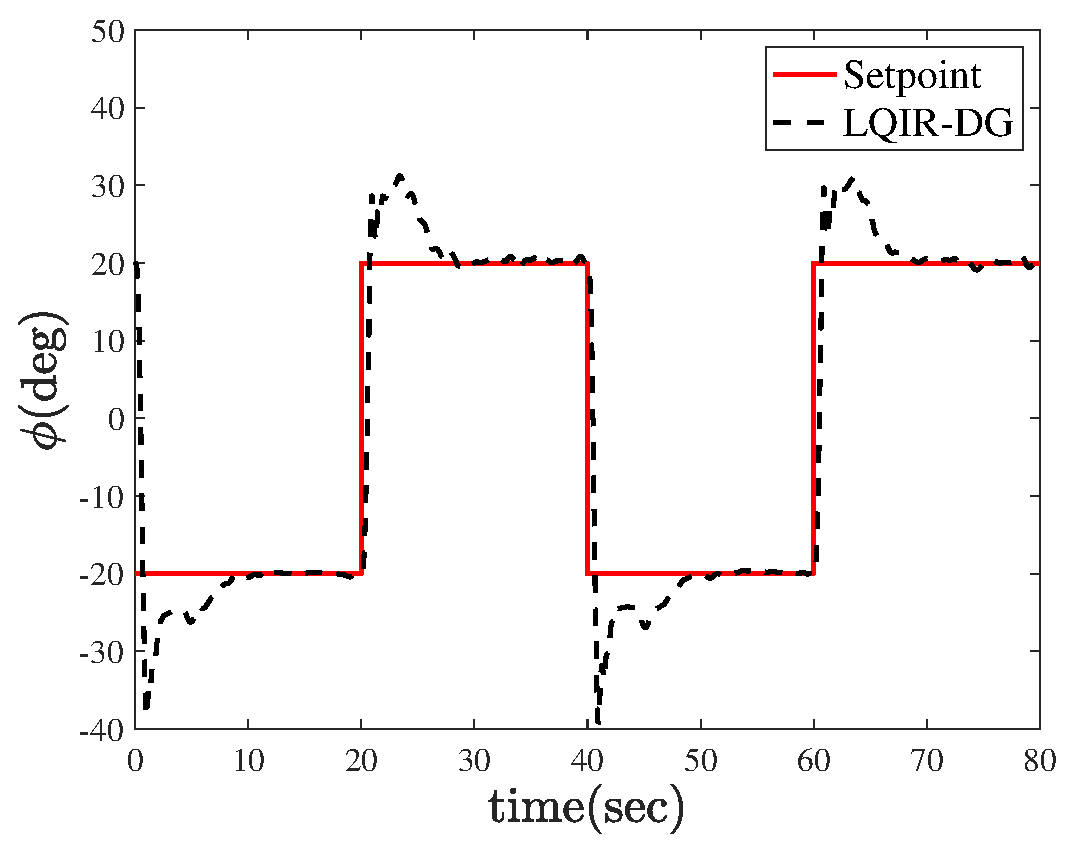
\includegraphics[width=.3\linewidth]{../Figure/implementation/square/lqidg_roll_20}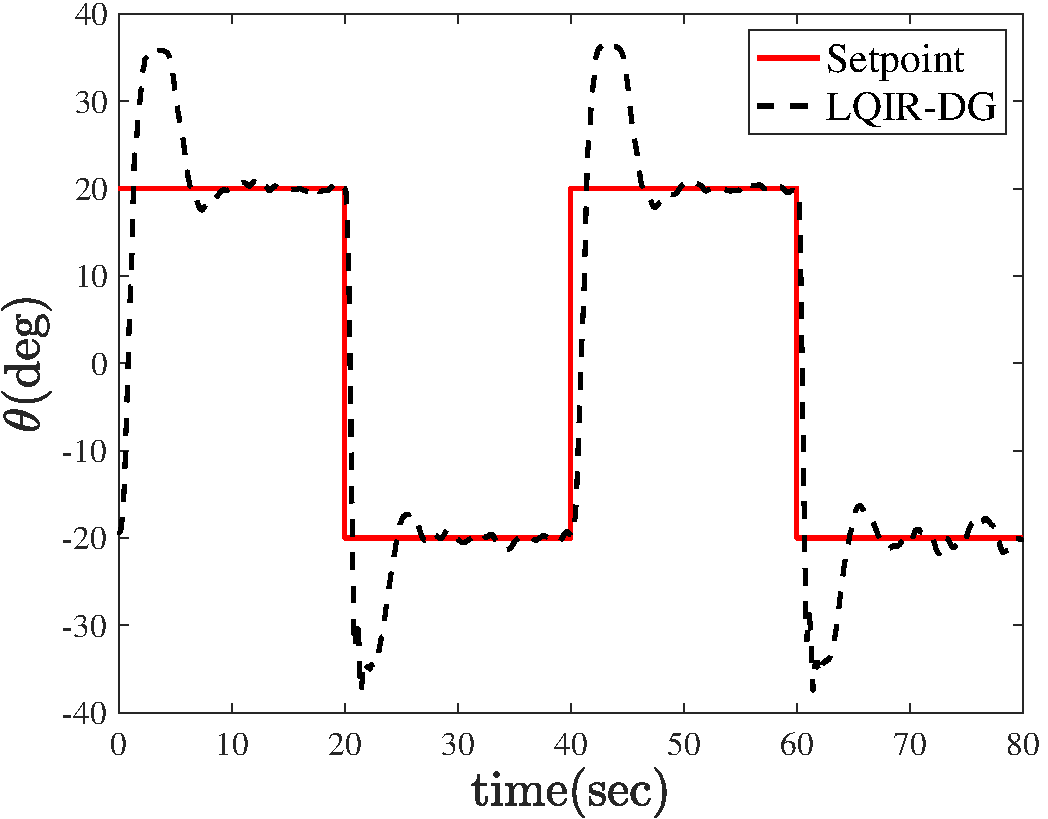
\includegraphics[width=.3\linewidth]{../Figure/implementation/square/lqidg_pitch_20}}
	\caption{Comparison of Euler angles in \ref{sub@fig:regulation} regulation \ref{sub@fig:square} Tracking Conditions}
	\label{fig:result}
\end{figure}

\begin{figure}[H]
	\centering
	\subfloat[\label{fig:omega_regulation}]{\includegraphics[width=.23\linewidth]{../Figure/implementation/lqidg_Omega_1}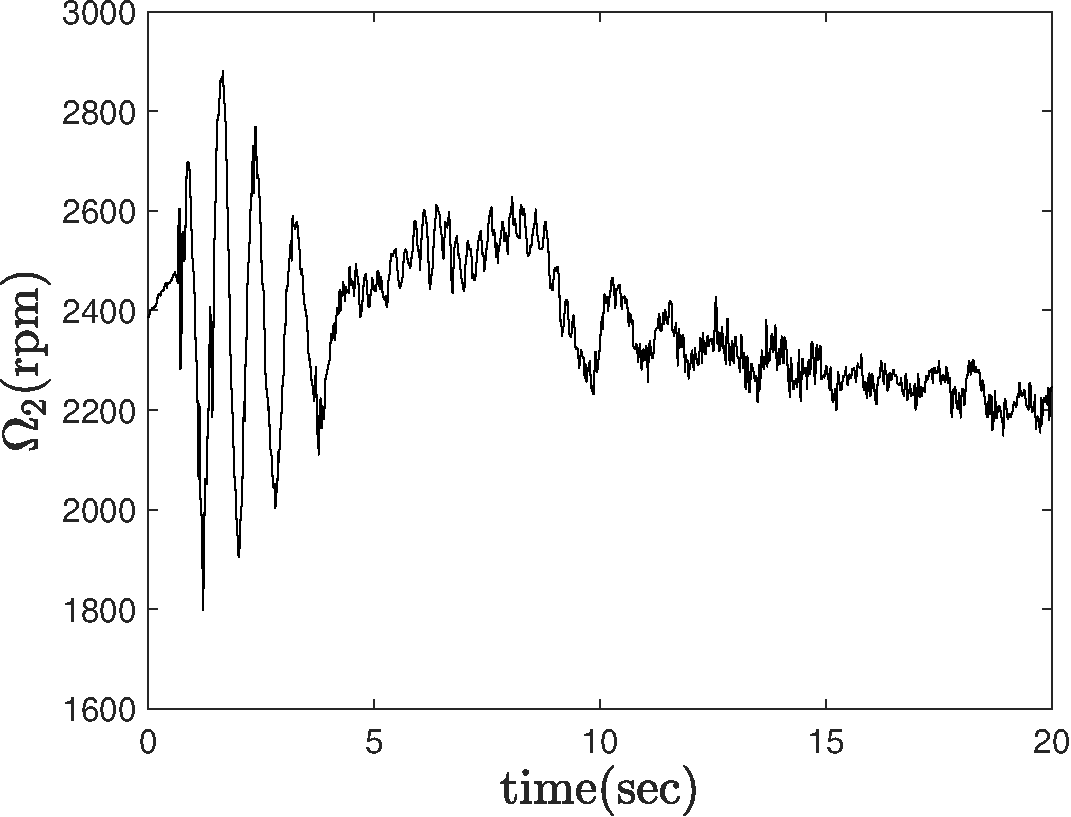
\includegraphics[width=.23\linewidth]{../Figure/implementation/lqidg_Omega_2}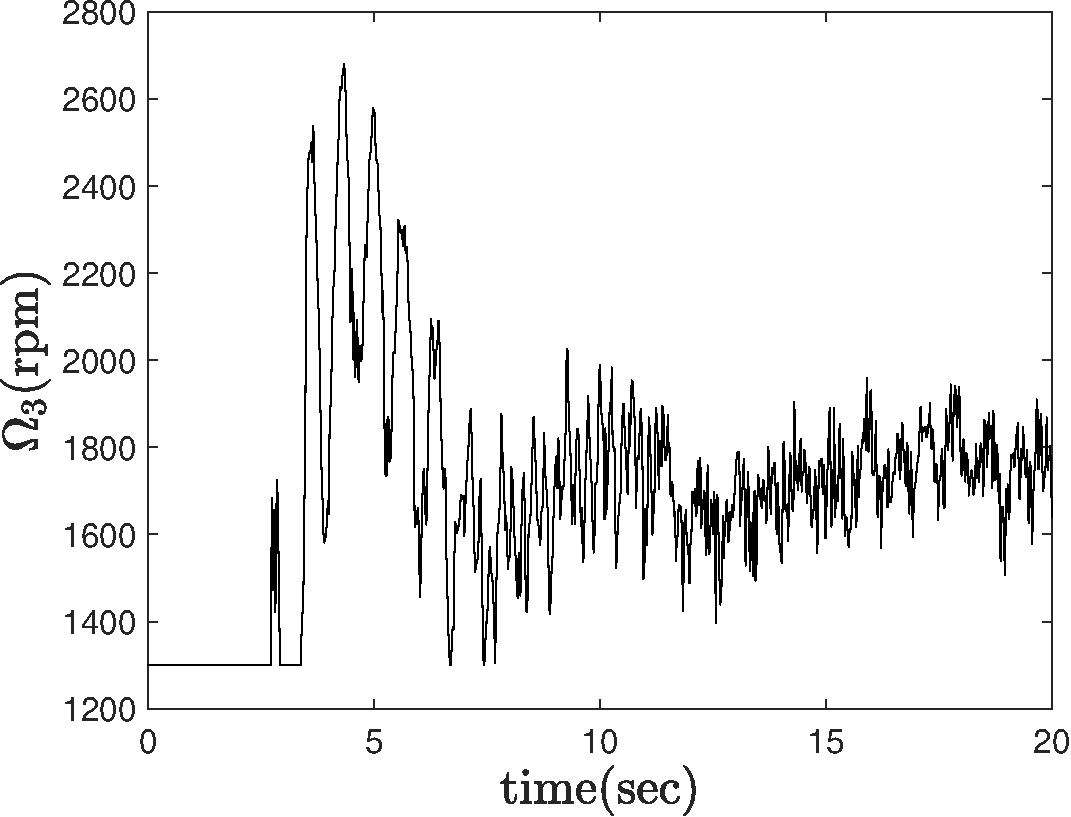
\includegraphics[width=.23\linewidth]{../Figure/implementation/lqidg_Omega_3}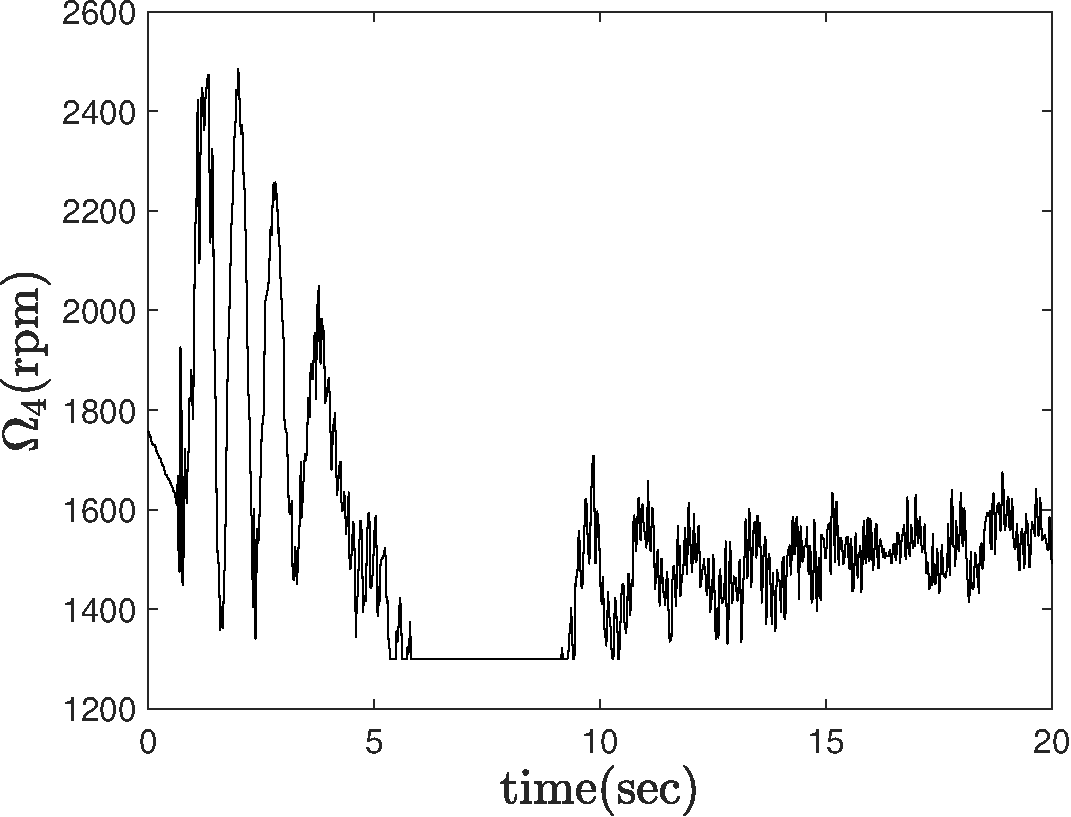
\includegraphics[width=.23\linewidth]{../Figure/implementation/lqidg_Omega_4}
	}
	\hfil
	\subfloat[\label{fig:omega_square}]{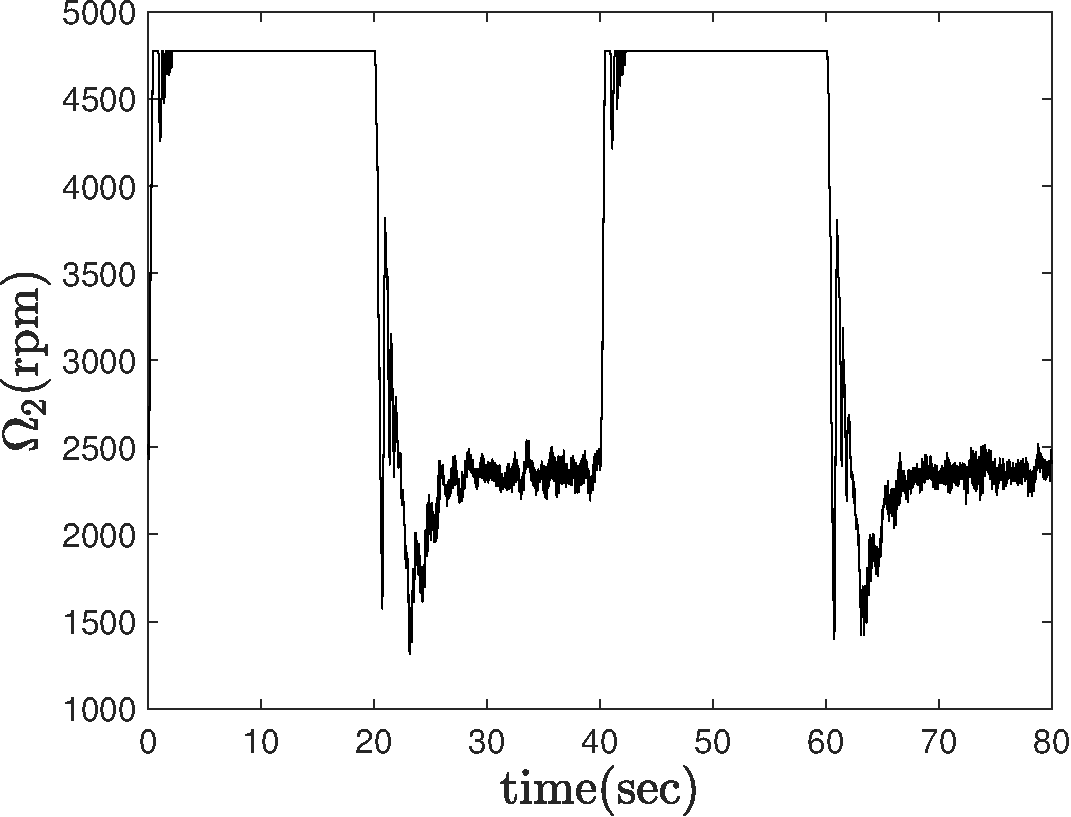
\includegraphics[width=.23\linewidth]{../Figure/implementation/square/lqidg_squre_omega_2}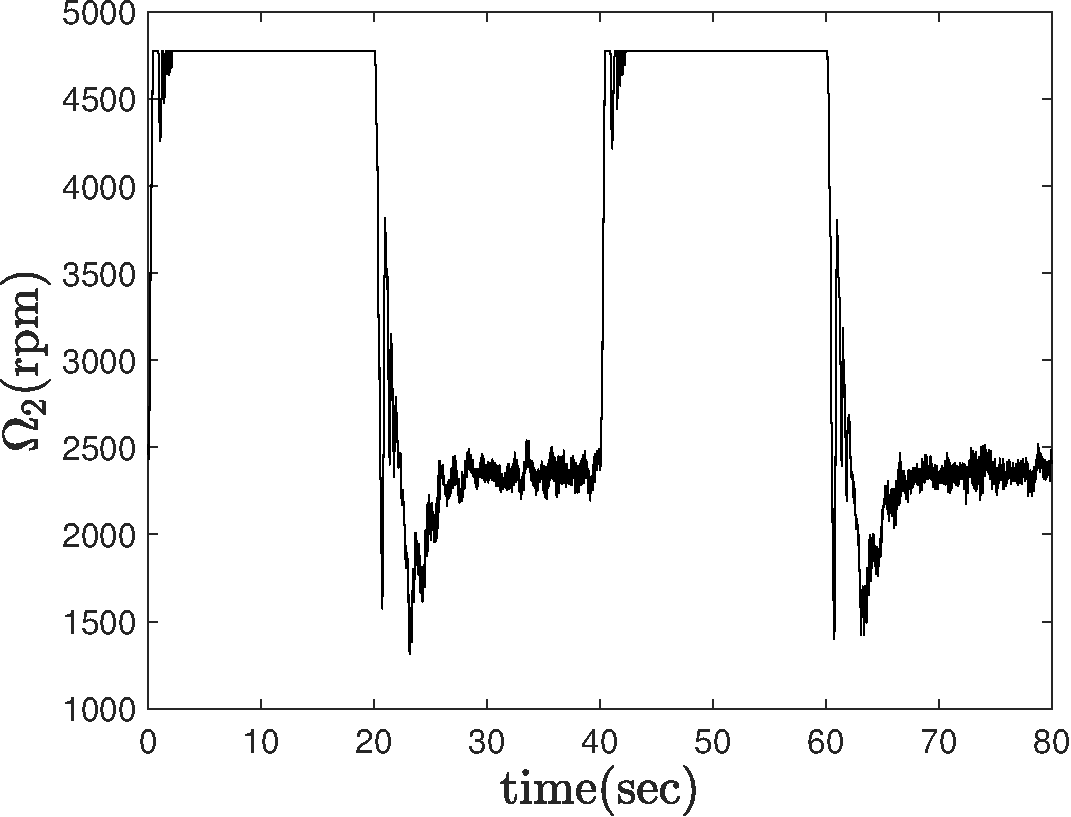
\includegraphics[width=.23\linewidth]{../Figure/implementation/square/lqidg_squre_omega_2}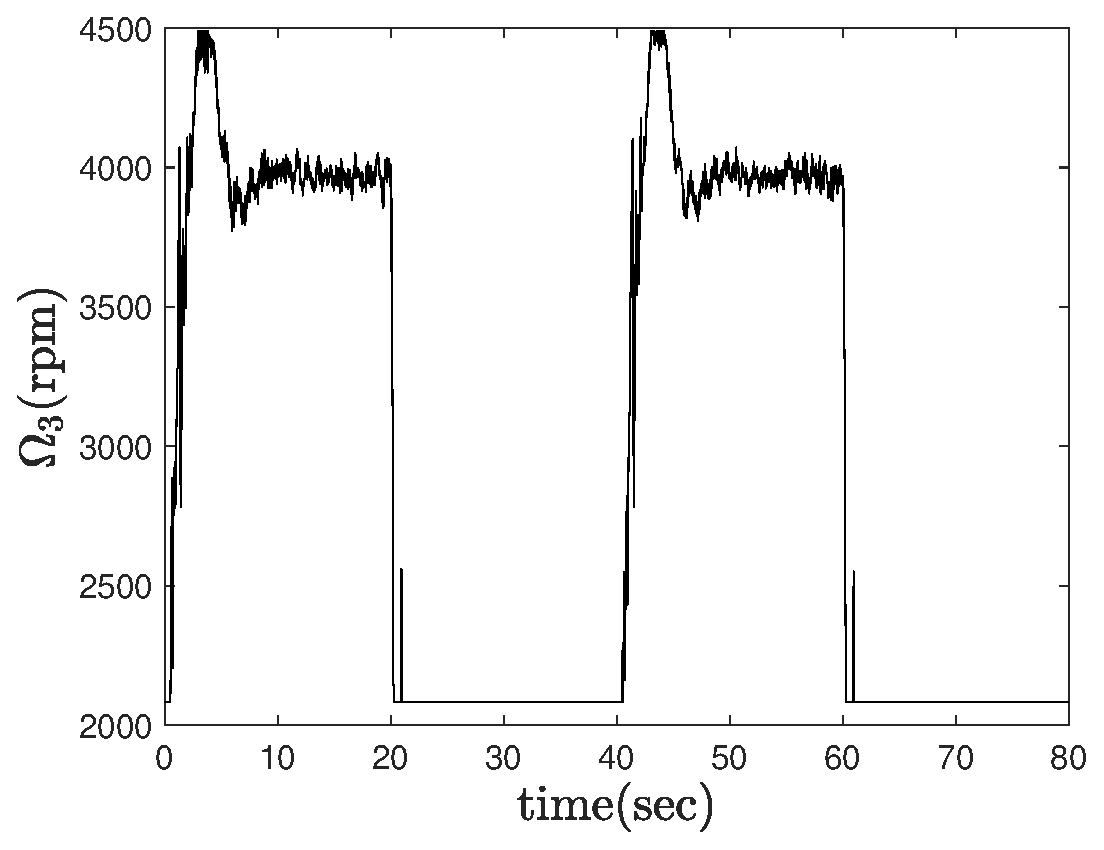
\includegraphics[width=.23\linewidth]{../Figure/implementation/square/lqidg_squre_omega_3}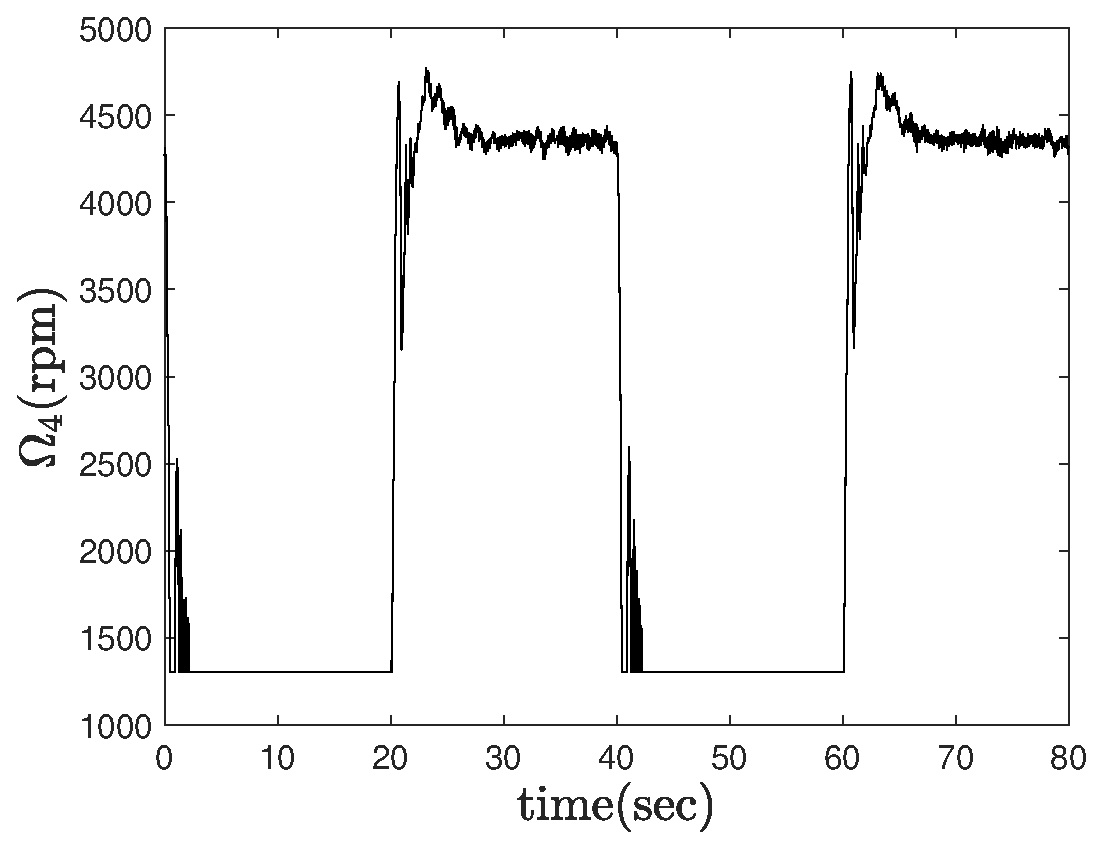
\includegraphics[width=.23\linewidth]{../Figure/implementation/square/lqidg_squre_omega_4}}
	\caption{Temporal Evolution of Angular Velocity Commands for the LQIR-DG Controller}
	\label{fig:omega}
\end{figure}


% Figure \ref{fig:square} The results of this experiment demonstrate the efficacy of the LQIR-DG control strategy in regulating the coupled roll and pitch channels, enabling accurate tracking of a desired square wave input with a frequency of 0.02 Hz and an amplitude of 20 degrees.


% \begin{figure}[H]
% 	\centering
% 	\subfloat[\label{fig:square_roll}]{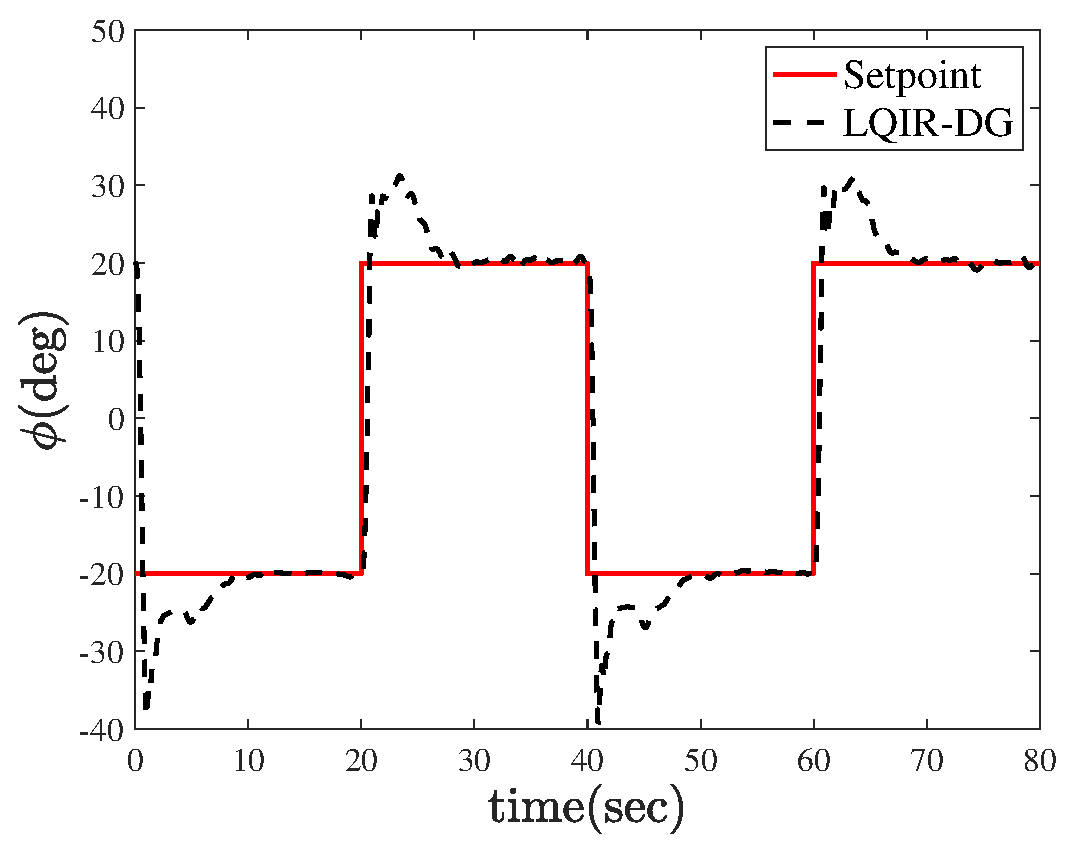
\includegraphics[width=.49\linewidth]{../Figure/implementation/square/lqidg_roll_20}}\subfloat[\label{fig:square_pitch}]{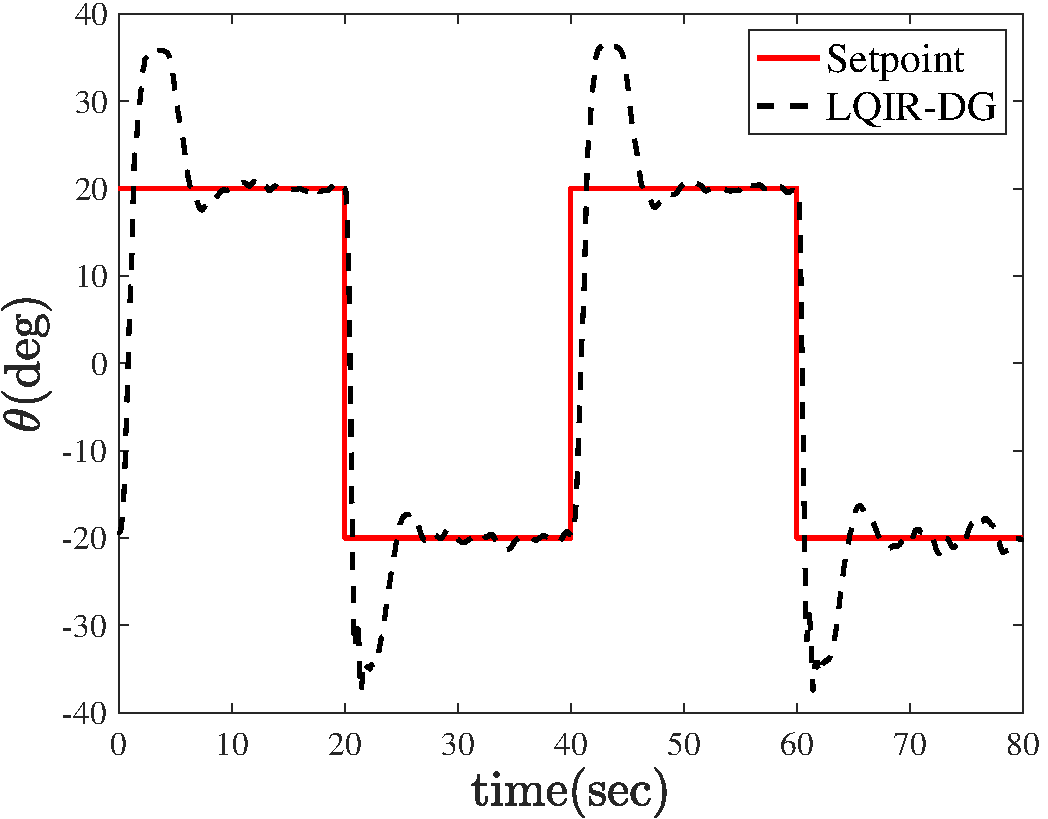
\includegraphics[width=.49\linewidth]{../Figure/implementation/square/lqidg_pitch_20}
% 	}
% 	\caption{Performance Evaluation of the LQIR-DDG Control Strategy for Tracking Desired Angles in the Two-Degree-of-Freedom Coupling Mode. Subfigure \ref{sub@fig:square_roll} displays the comparison between the actual and desired roll angles, while subfigure \ref{sub@fig:square_pitch} shows the comparison between the actual and desired pitch angles.}
% 	\label{fig:square}
% \end{figure}

\subsubsection{Performance of the LQIR-DG in Disturbance Rejection}\label{sec:disturbance}

% \noindent This section investigates the possible rejection of input disturbances by the LQIR-DG controller in regulation. For this purpose, a disturbance with an amplitude of 0.5 N is added to the input from 20 to 60 seconds. As shown in figure \ref{fig:disturbance}, the LQIR-DG controller performs well in coupling the roll and screw channels to remove the input disturbance. \ref{fig:disturbance}\ref{sub@fig:disturbance_roll}, the performance of this controller is checked by comparing the desired roll angle with the actual roll angle. Also, \ref{fig:disturbance}\ref{sub@fig:disturbance_pitch} compares the desired pitch angle with the actual pitch angle of the 3DoF experimental setup in removing the input disturbance. The results indicate the proper performance of the controller in removing the input disturbance.
% \noindent This section examines the effectiveness of the LQIR-DG controller in attenuating input disturbances during regulation. To this end, a disturbance with an amplitude of 0.5 N is added to the input signal from 20 to 60 seconds. As depicted in Figure \ref{fig:disturbance}, the LQIR-DG controller demonstrates proficient coupling of the roll and screw channels, resulting in effective removal of the input disturbance. Figure \ref{fig:disturbance}\ref{sub@fig:disturbance_roll} depicts an evaluation of the controller's performance through a comparison between the desired and actual roll angles, while Figure \ref{fig:disturbance}\ref{sub@fig:disturbance_pitch} presents a similar analysis for the desired and actual pitch angles. The results indicate that the LQIR-DG controller performs appropriately in mitigating the input disturbance.
\noindent The performance of the proposed controller in the input disturbance is shown in Figure \ref{fig:disturbance}. The input disturbance, $\mathrm{d\Omega_i}$, is considered as a change in the command of the rotational velocity, modeled as:
\begin{equation}
	\mathrm{d\Omega_1} = \mathrm{d\Omega_2} = -\mathrm{d\Omega_3} = -\mathrm{d\Omega_4} = \begin{cases}
		500_{\mathrm{rpm}} \quad &20<t<60\\
		0 \quad &\mathrm{other}
	\end{cases}
\end{equation}

Figure \ref{fig:disturbance} \ref{sub@fig:disturbance_angle} illustrate the desired and the actual roll and pitch angles in the regulation problem. The results indicate that the LQIR-DG controller can stabilize the quadrotor platform when the input disturbance is present.

\begin{figure}[H]
	\centering
	\subfloat[\label{fig:disturbance_angle}]{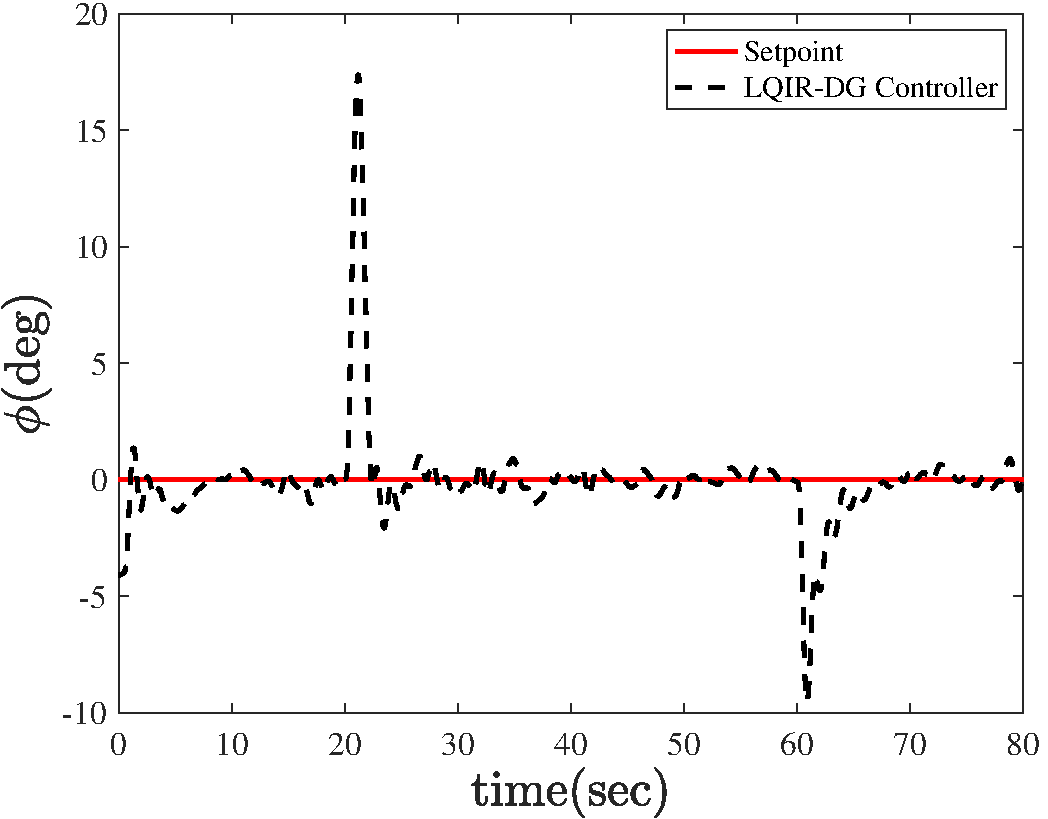
\includegraphics[width=.49\linewidth]{../Figure/implementation/disturbance/lqidg_roll}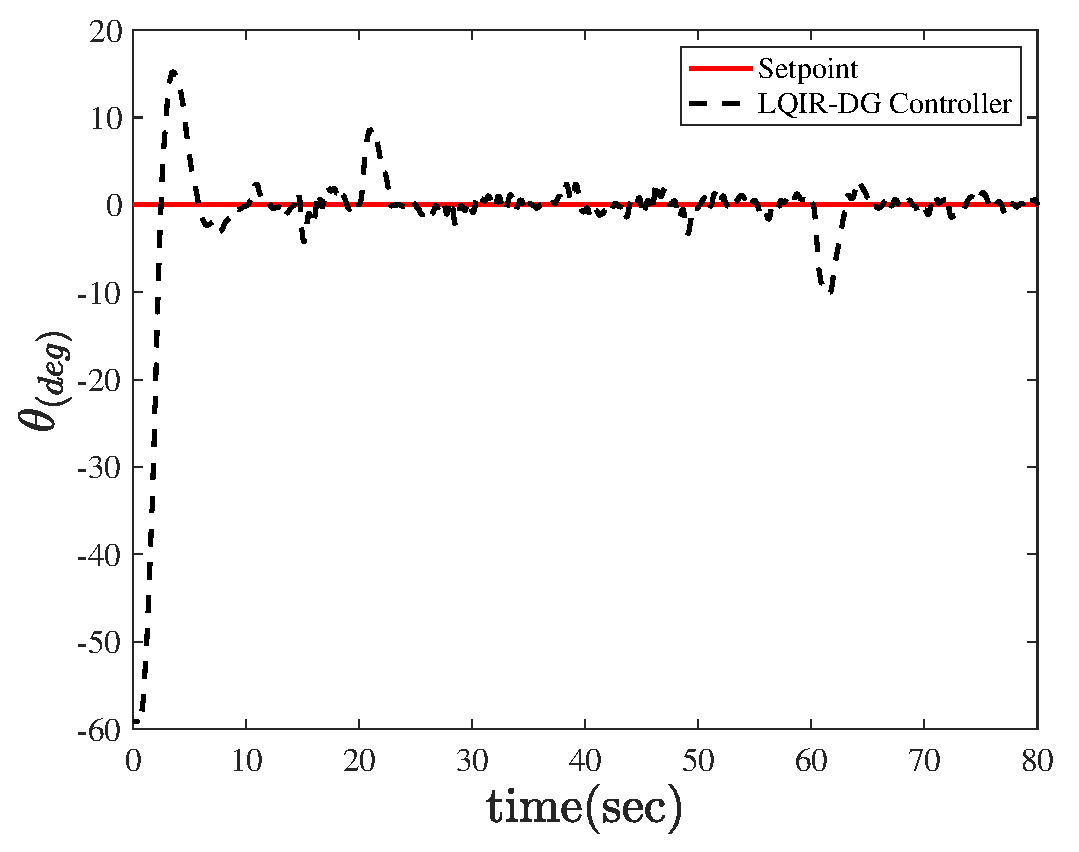
\includegraphics[width=.49\linewidth]{../Figure/implementation/disturbance/lqidg_pitch}
	}
	% \hfill
	% \subfloat[\label{fig:omega_disturbance}]{\includegraphics[width=.23\linewidth]{../Figure/implementation/disturbance/lqidg_Omega_1}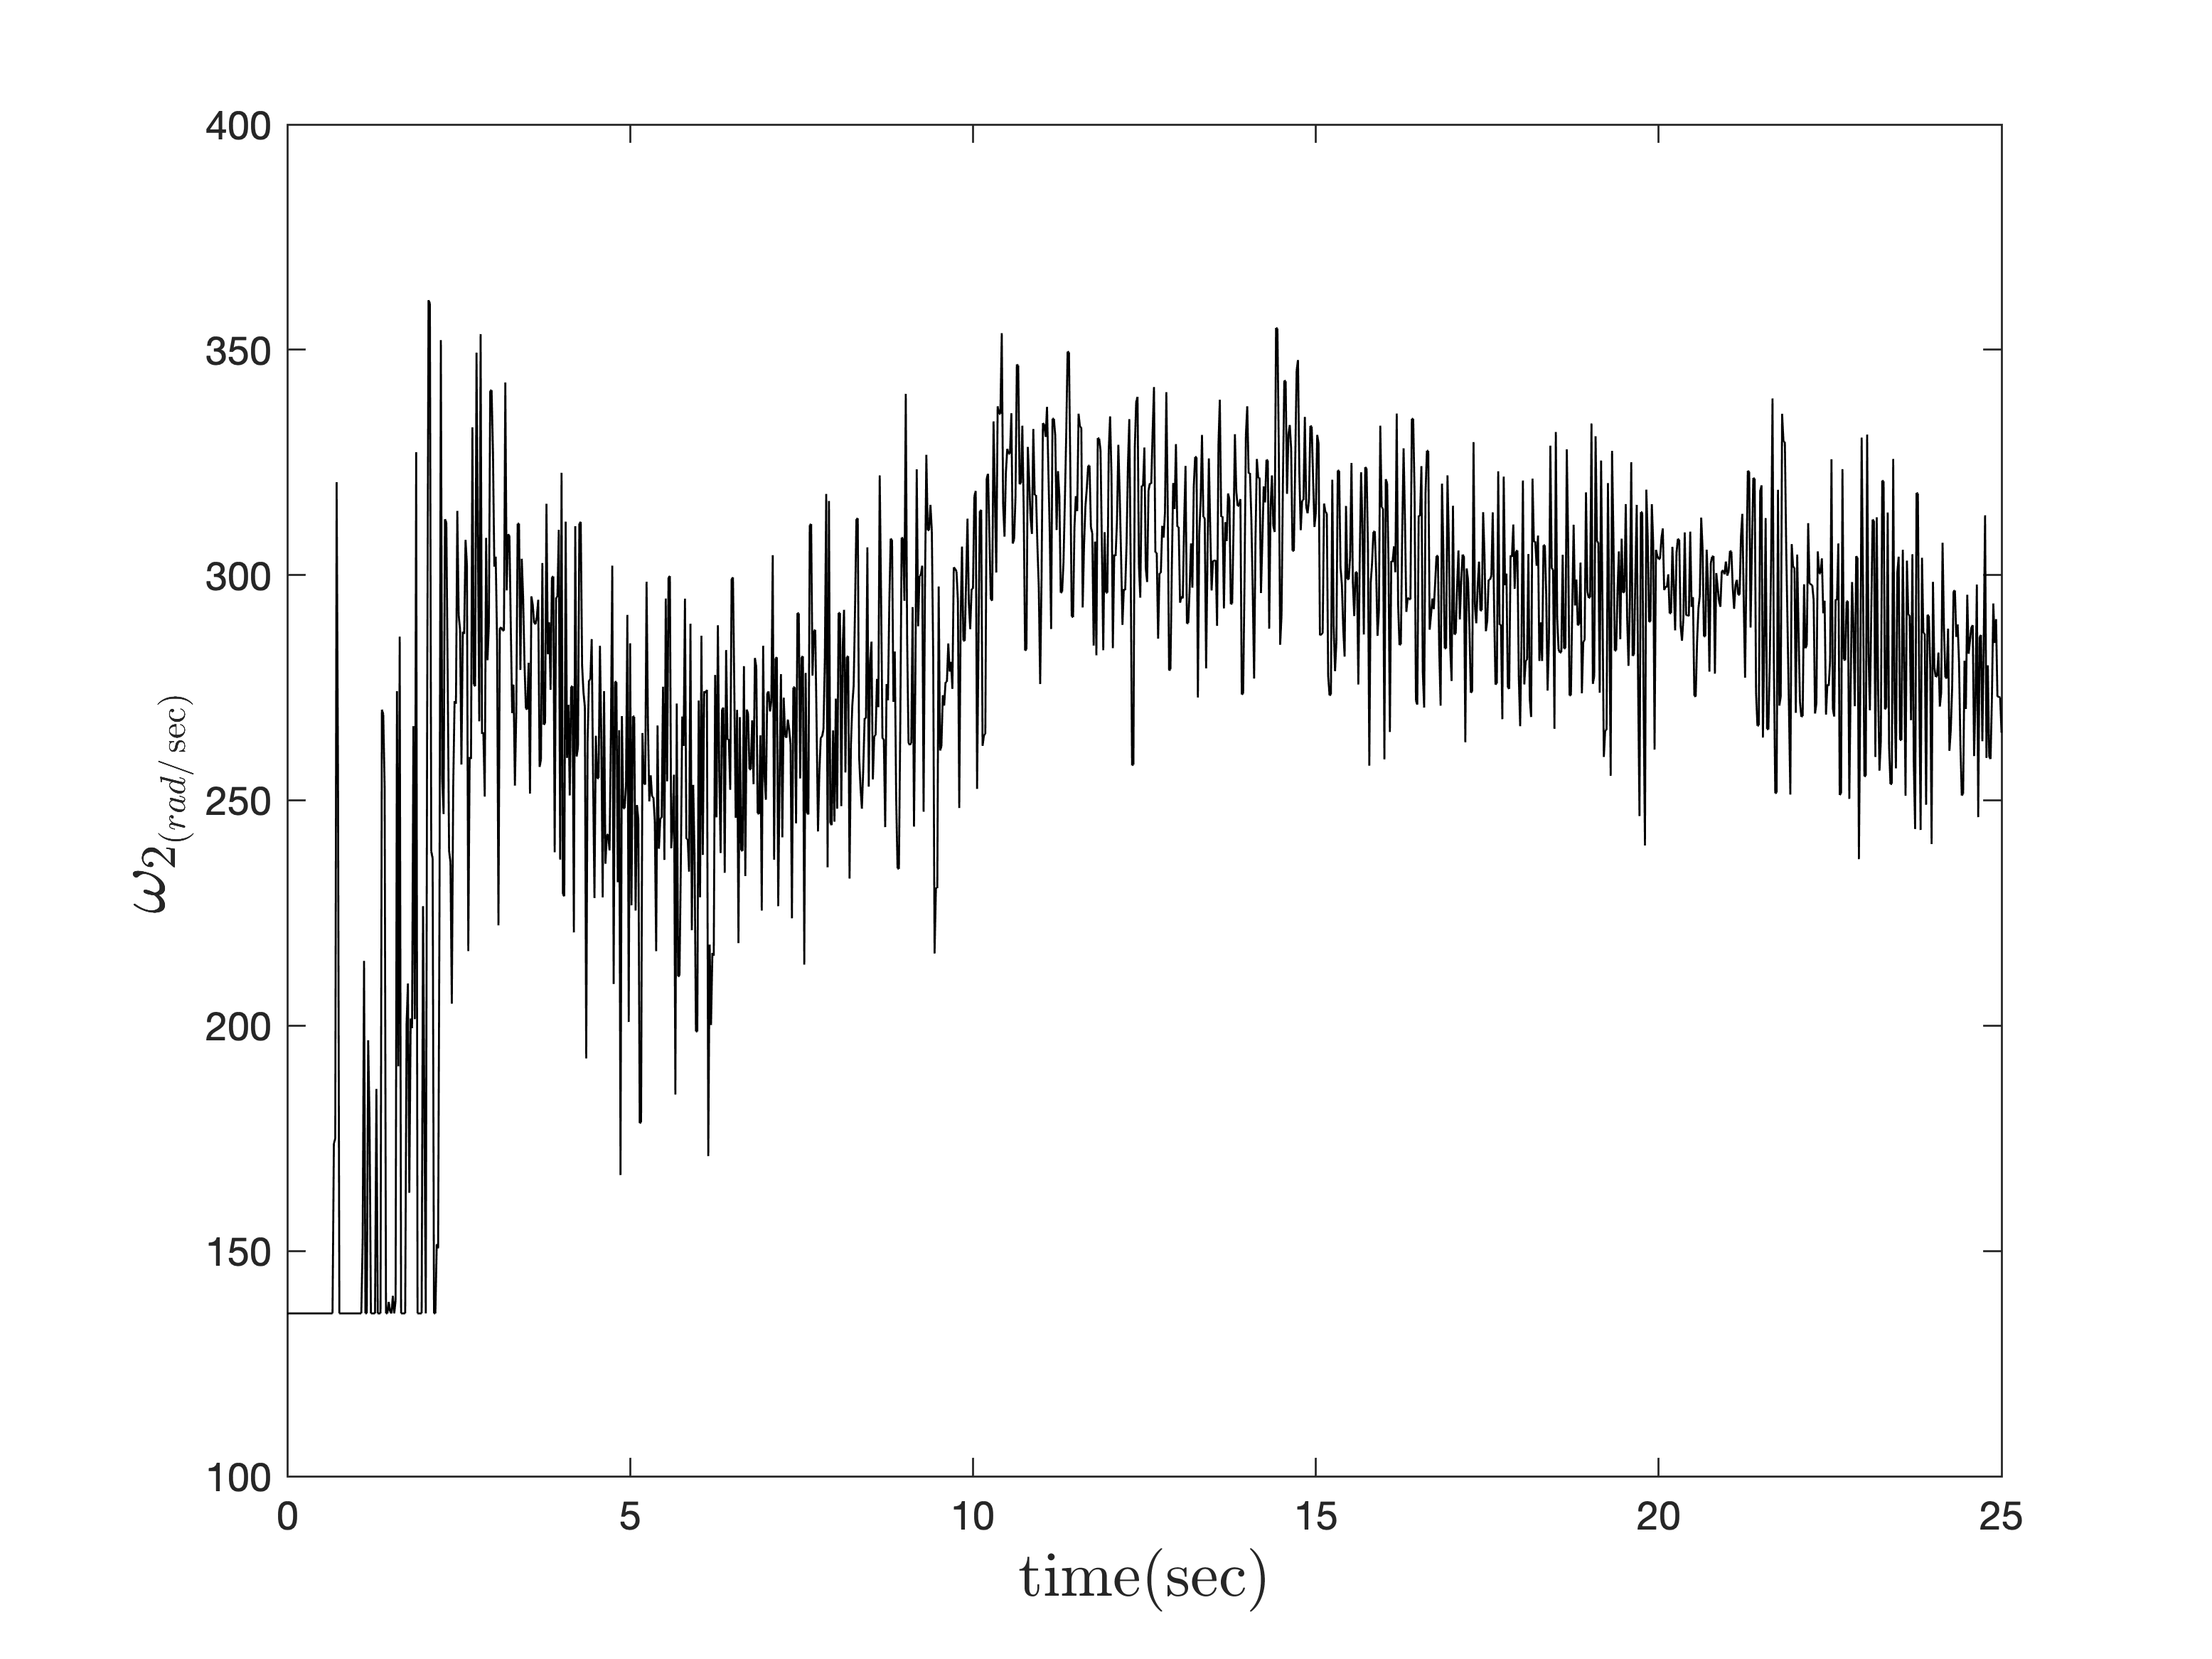
\includegraphics[width=.23\linewidth]{../Figure/implementation/disturbance/lqidg_Omega_2}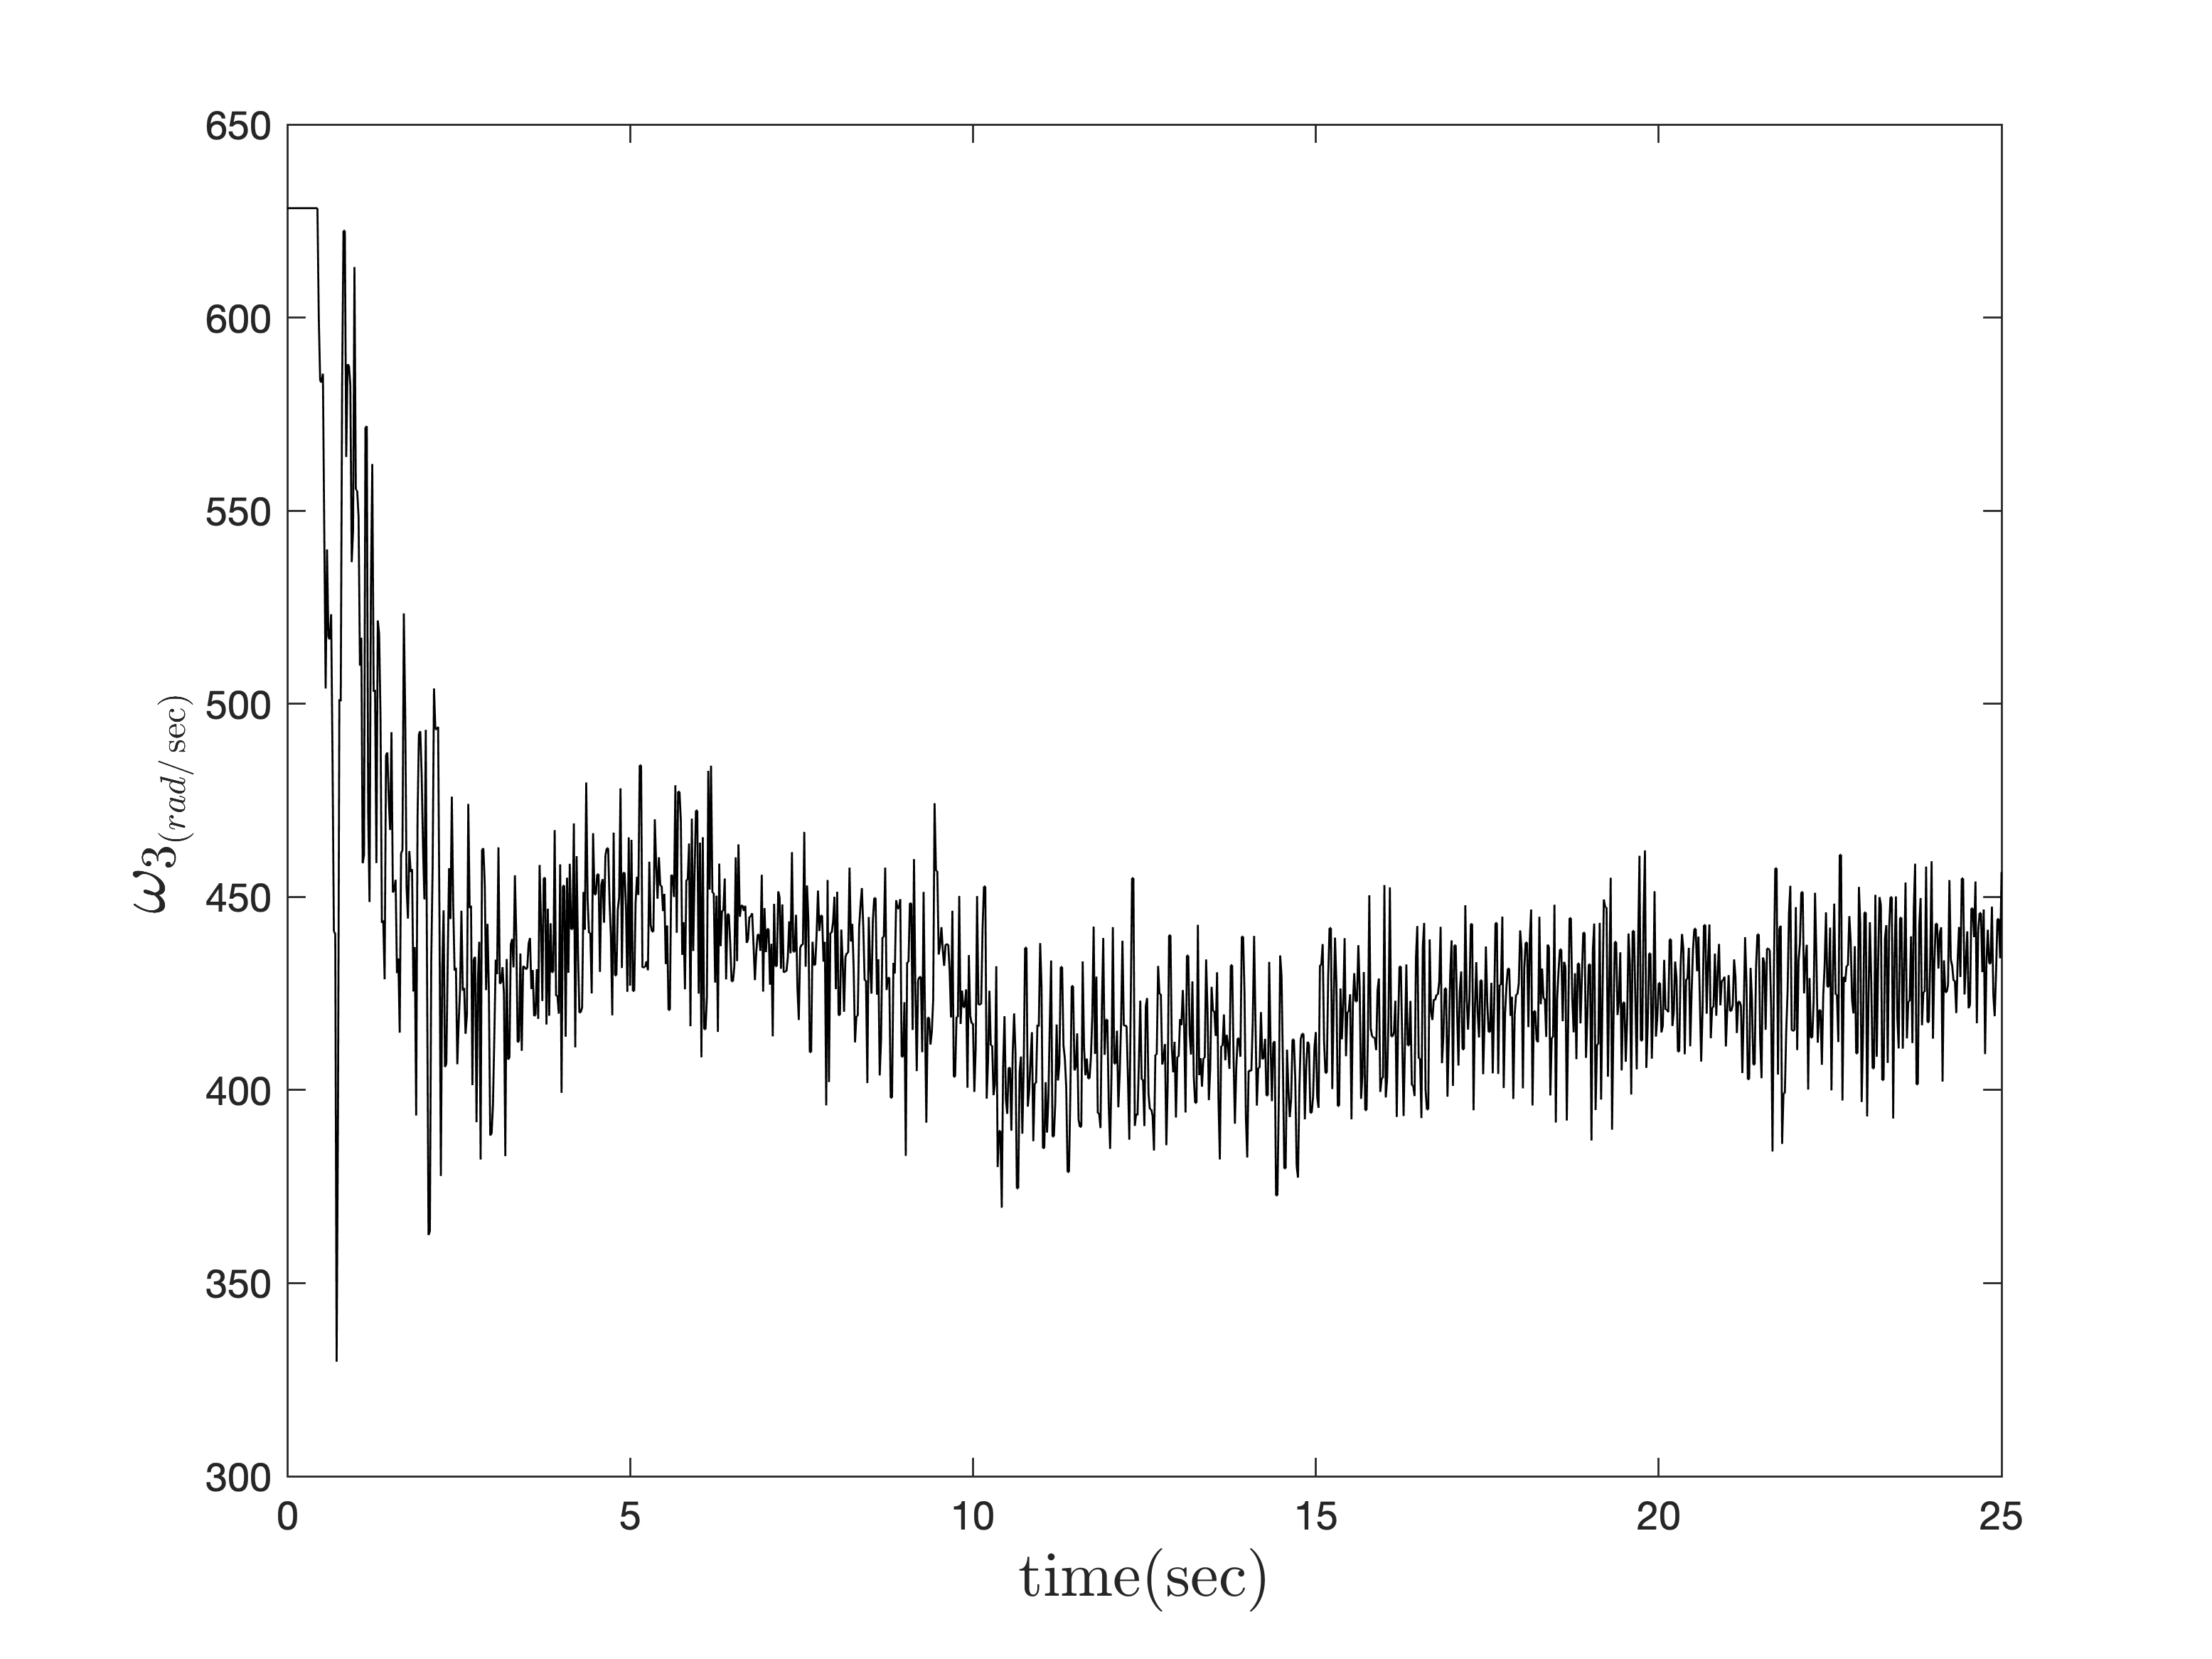
\includegraphics[width=.23\linewidth]{../Figure/implementation/disturbance/lqidg_Omega_3}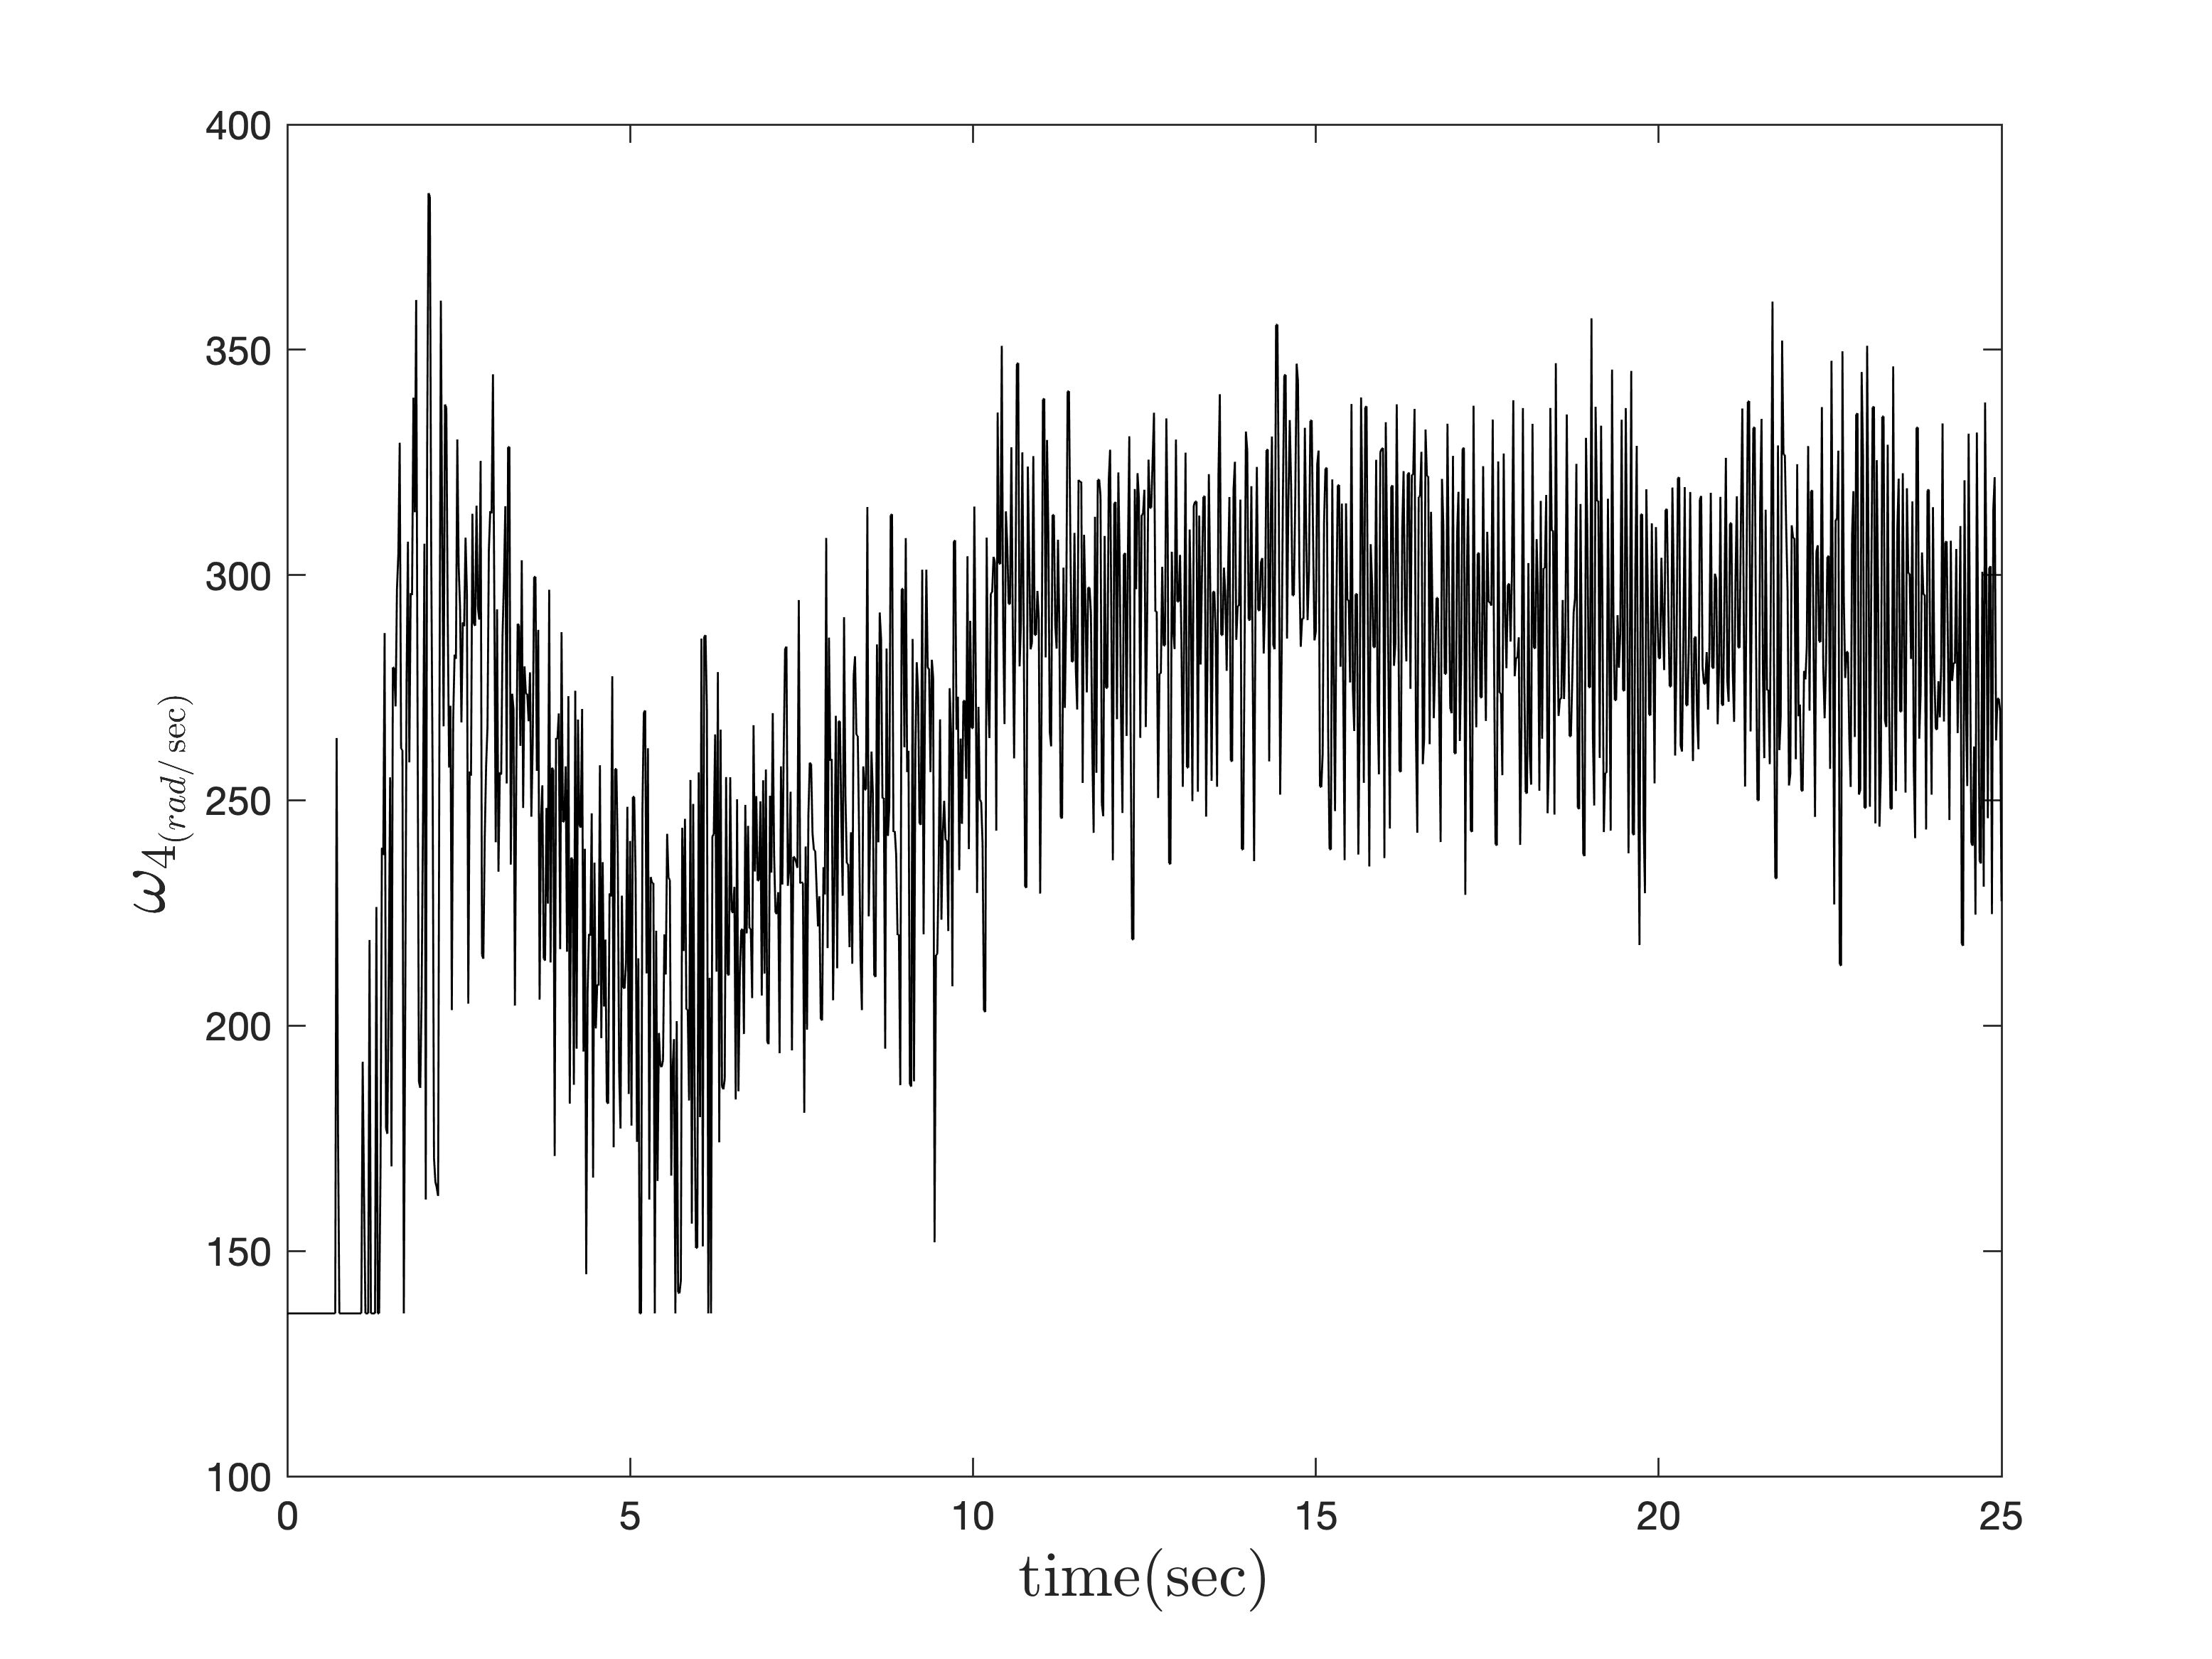
\includegraphics[width=.23\linewidth]{../Figure/implementation/disturbance/lqidg_Omega_4}}
	% \hfil
	% \subfloat[]{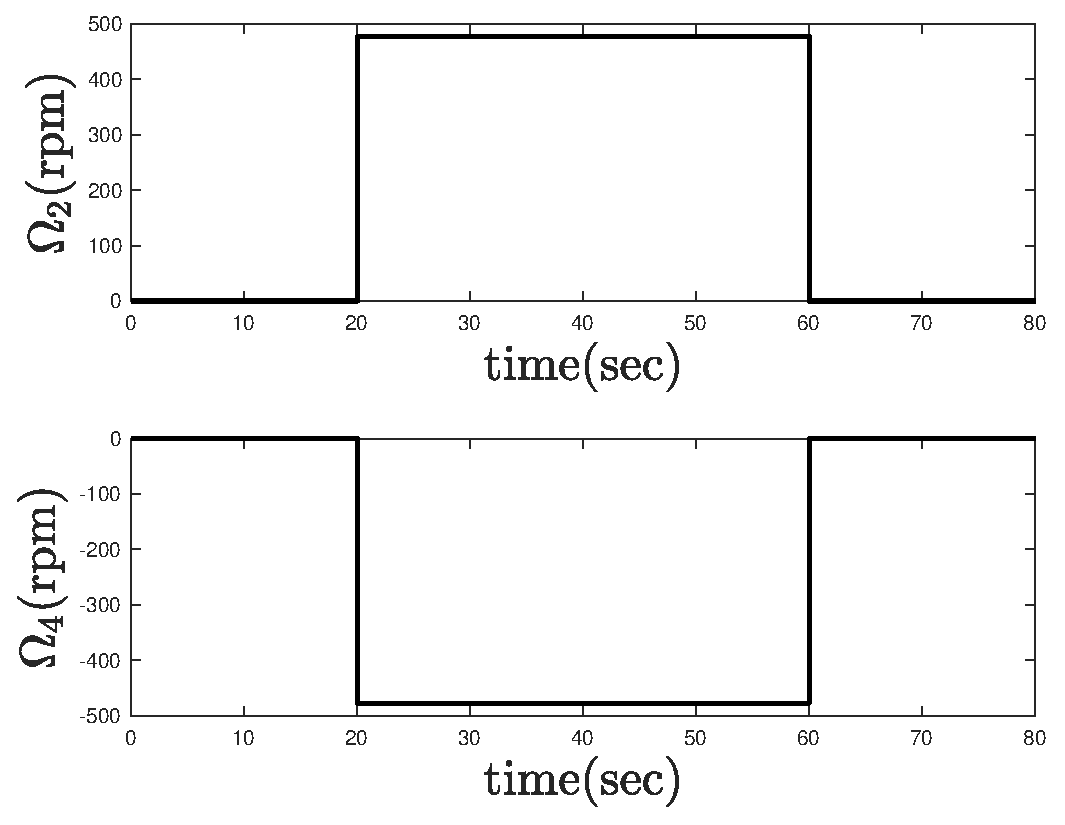
\includegraphics[width=.49\linewidth]{../Figure/implementation/disturbance/d_roll}}\subfloat[]{\includegraphics[width=.49\linewidth]{../Figure/implementation/disturbance/d_pitch}
	% }
	\caption{Comparison of the desired and actual roll and pitch angle in the presence of the input disturbance.}
	\label{fig:disturbance}
\end{figure}

\subsubsection{Investigating the Impact of Modeling Uncertainty}\label{sec:model-uncertainty}
% \noindent In this section, the performance of the LQIR-DG controller is investigated under the consideration of uncertainty in the 3DoF experimental model. Specifically, the controller's effectiveness in the coupling mode of the roll and pitch channels is evaluated while taking into account the uncertain values of the moments of inertia around each axis of the body coordinate system. The results of this investigation are presented in figure \ref{fig:weight}, where a disturbance of 50 grams is added to the roll axis and 100 grams to the pitch axis.
\noindent In this section, the performance of the LQIR-DG controller is investigated while considering uncertainty in the 3DoF experimental model. 
To achieve this, 50 and 100 grams were added to the roll and pitch axes, respectively, as shown in Figure \ref{fig:quadrotor_with_weight}.
% \noindent In this section, the performance of the LQIR-DG controller is investigated under the consideration of uncertainty in the 3DoF experimental model. For this purpose, according to Figure \ref{fig:quadrotor_with_weight}, 50 and 100 grams are added to the roll and pitch axes, respectively.
% Figure \ref{fig:weight}\ref{sub@fig:weight_roll} and \ref{sub@fig:weight_pitch} depict the evaluation of the LQIR-DG controller with emphasis on the comparison of desired and actual roll and pitch angles, respectively. The implementation results indicate that the LQIR-DG controller performs efficiently in achieving the desired values, even with the uncertainty in the moments of inertia.
Figure \ref{fig:weight} \ref{sub@fig:weight_roll} compares the desired and the actual roll angle and Figure \ref{fig:weight} \ref{sub@fig:weight_pitch} shows the desired and the actual pitch angle when the uncertainty of moments of inertia is presented.
Moreover, Figure \ref{fig:weight} \ref{sub@fig:omega_weight} shows the rotational velocity command of the experimental platform in the presence of model uncertainty.
The implementation results indicate that the LQIR-DG controller converges to the desired values in the presence of the modeling uncertainty.


\begin{figure}[H]
	\centering
	\includegraphics[width=0.49\textwidth]{../Figure/implementation/weight/Quad_with_weight.jpg}
	\caption{Quadrotor 3DoF Platform with Added Weight.}
	\label{fig:quadrotor_with_weight}
 \end{figure}
\begin{figure}[H]
	\centering
	\subfloat[\label{fig:weight_roll}]{\includegraphics[width=.49\linewidth]{../Figure/implementation/weight/lqidg_roll_20}}\subfloat[\label{fig:weight_pitch}]{\includegraphics[width=.49\linewidth]{../Figure/implementation/weight/lqidg_pitch_20}
	}
	\hfill
	\subfloat[\label{fig:omega_weight}]{\includegraphics[width=.23\linewidth]{../Figure/implementation/weight/lqidg_Omega_1}\includegraphics[width=.23\linewidth]{../Figure/implementation/weight/lqidg_Omega_2}\includegraphics[width=.23\linewidth]{../Figure/implementation/weight/lqidg_Omega_3}\includegraphics[width=.23\linewidth]{../Figure/implementation/weight/lqidg_Omega_4}}
	\caption{Comparison of the LQIR-DG controller when the uncertainty of moment of inertia is presented}
	\label{fig:weight}
\end{figure}

\subsubsection{Comparison with the Control Strategies}
% \noindent Here, the LQIR-DG controller performance is compared with famous control strategies such as the LQR controller method. \figurename{\ref{fig:compare}} compares the quadrotor's desired and actual pitch angle in the presence of these controllers. This result indicates that the LQIR-DG controller can provide high tracking performance, such as good transient response and high rapid convergence relative to the LQR controller for pitch angle control of the quadrotor setup.
% \noindent This section compares the implementation performance of three different controllers for the quadrotor system: PID, LQR, and LQIR-DG. The comparison is made based on the implementation results of the controllers in the presence of uncertainty, input disturbance, and weight addition in the two-degree-of-freedom coupling mode.
% The PID controller has been widely used in quadrotor control due to its simplicity and ease of implementation. However, its performance is limited in complex scenarios due to the inherent nonlinearity and uncertainty of the quadrotor system.

% The LQR and LQIR controller is a linear feedback control method that can provide better performance than PID by optimizing a quadratic cost function. However, it requires an accurate model of the system, and is sensitive to uncertainties and disturbances in the system.

% The LQIR-DG controller, which is based on game theory, considers both the system dynamics and the measurement uncertainties, and provides better performance in the presence of uncertainty and disturbances. In addition, the LQIR-DG controller can handle weight additions without requiring a re-design of the controller.

% The implementation results indicate that the LQIR-DG controller outperforms the PID and LQR controllers in terms of accuracy and robustness in the presence of uncertainties and disturbances. The comparison results for the three controllers are summarized as follows:

% \begin{itemize}
% 	\item PID \newline
% 	The PID controller can track the desired angles reasonably well in the absence of uncertainties and disturbances. However, its performance is significantly affected by the presence of uncertainty and disturbances, resulting in oscillations and overshoots in the response.
% 	\item LQR and LQIR \newline
% 	The LQR and LQIR controller provides better performance than PID in the absence of uncertainties and disturbances. However, it is more sensitive to system uncertainties and disturbances, resulting in larger errors and oscillations in the response.
% 	\item LQIR-DG \newline
% 	Among the three controllers compared, the LQIR-DG controller exhibits superior performance, exhibiting robustness to uncertainties, disturbances, and weight additions without necessitating a re-design of the control system. The LQIR-DG controller provides accurate and robust control of the quadrotor system, with minimal errors and oscillations in the response.
% \end{itemize}

% In summary, the LQIR-DG controller provides better performance than PID and LQR controllers, and is a promising control method for quadrotor systems in the presence of uncertainties and disturbances.

\noindent Here, the LQIR-DG controller performance is compared with the PID controller and variant of the LQR strategies such as the LQR and LQIR in Figure \ref{fig:compare}. 
Figure \ref{fig:compare} compare the desired and the actual attitude of the quadrotor platform in the presence of these controllers.
Moreover, the RSME of the controllers of all the controllers, i.e, boxplot, are compared in Figure \ref{fig:compare_boxplot}. 
The median of RMSE is shown in the crossline in the boxplot.

These results indicate that the LQIR-DG controller is able to provide an excellent transient response and rapid convergence relative to other controllers for attitude control of the quadrotor experimental platform.



\begin{figure}[H]
	\centering
	\subfloat[\label{fig:all_roll}]{\includegraphics[width=.49\linewidth]{../Figure/implementation/lqidgvslqr/roll}}\subfloat[\label{fig:all_pitch}]{\includegraphics[width=.49\linewidth]{../Figure/implementation/lqidgvslqr/pitch}
	}
	\caption{Comparison of LQIR-DG Controller to the LQR, LQIR, and PID in control of the quadrotor outputs: (a) roll angle (b) pitch angle.}
	\label{fig:compare}
\end{figure}

\begin{figure}[H]
	\centering
	{\includegraphics[width=.49\linewidth]{../Figure/implementation/box_plot/lqidgvsboxplot}
	}
	\caption{Comparative Analysis of the LQIR-DG Control Strategy versus LQR, LQIR, and PID Controllers using Quadratic Cost Function}
	\label{fig:compare_boxplot}
\end{figure}


\section{Conclusion}\label{sec:conclusion}
% \noindent In this study, a linear quadratic with integral action based on the differential game theory, called LQIR-DG, was implemented for level attitude control in an experimental setup of a quadrotor. To implement the proposed controller structure, first, an accurate model of the quadrotor was linearized in the state-space form, and then the model parameters were estimated. Next, two players were considered for each of the quadrotor's roll, pitch, and yaw channels. The first player found the best control command for each channel of the setup of a quadrotor based on the mini-maximization of a quadratic criterion; when the second player produced the worst disturbances. Finally, the performance of the proposed controller was investigated in level flight and compared to the LQR controller. The implementation results verify the successful performance of the LQIR-DG method in the level flight of the attitude control and tracking sware wave and disturbance rejection and model uncertainty for the actual plant.

% \noindent This study presented the implementation and evaluation of a linear quadratic with integral action based on the differential game theory, named LQIR-DG, for level attitude control in an experimental setup of a quadrotor. The proposed controller structure required the linearization of an accurate model of the quadrotor in the state-space form and the estimation of the model parameters. The design of the LQIR-DG controller involved two players for each of the quadrotor's roll, pitch, and yaw channels. The first player optimized the control command for each channel based on the mini-maximization of a quadratic criterion, while the second player generated the worst disturbances. The evaluation of the LQIR-DG method was conducted in level flight and compared to the LQR controller. The results demonstrated the successful performance of the LQIR-DG method in level flight of the attitude control and tracking square wave, disturbance rejection, and model uncertainty in the actual plant.
% \noindent This study has introduced a novel methodology for the implementation and assessment of a controller with integral action utilizing linear quadratic optimization, founded on the principles of differential game theory, with the aim of achieving level attitude control and reference tracking in an experimental platform of the quadrotor.
% The development of the proposed controller design necessitated the formulation of a precise state-space model for the quadrotor, which was then linearized. The estimation of the model parameters was subsequently conducted in accordance with the design process.
% The implementation of the LQIR-DG controller required the coordination of two players, with each player dedicated to controlling a specific Euler angle channel.
% The first player, utilizing a quadratic criterion, performed optimization of the control input for each channel, while another player makes the most challenging disturbances.

% The efficacy of the LQIR-DG control strategy was assessed in hover and compared against the PID, LQR, and LQIR controllers. The experimental findings demonstrated the efficacy of the LQIR-DG approach for achieving attitude control, square wave tracking, disturbance rejection, and robustness to model uncertainty in the actual quadrotor platform during level flight. Overall, this study has demonstrated the effectiveness and potential of the LQIR-DG method in quadrotor attitude control, which can be extended to other aerospace systems.
\noindent In this paper, the LQIR-DG method, which is an optimal controller based on the game theory, was used in real-time for attitude control of an experimental platform for a quadrotor.
To implement the proposed controller, an accurate dynamic model was considered for the quadrotor platform.
Then, the model parameters were identified using the NSL method.
For evaluation of the proposed method, the purpose of regulation and tracking problem was successfully performed.
Moreover, the method's ability to reject the input disturbance and modelling error was investigated in the laboratory experiment.
The implementation results illustrated the successful performance of the proposed method in attitude control for the quadratic platform.





%% The Appendices part is started with the command \appendix;
%% appendix sections are then done as normal sections
%% \appendix

%% \section{}
%% \label{}

%% References
%%
%% Following citation commands can be used in the body text:
%% Usage of \cite is as follows:
%%   \cite{key}         ==>>  [#]
%%   \cite[chap. 2]{key} ==>> [#, chap. 2]
%%

%% References with BibTeX database:

\bibliographystyle{elsarticle-num}
\bibliography{refs}

%% Authors are advised to use a BibTeX database file for their reference list.
%% The provided style file elsarticle-num.bst formats references in the required Procedia style

%% For references without a BibTeX database:

% \begin{thebibliography}{00}

%% \bibitem must have the following form:
%%   \bibitem{key}...
%%

% \bibitem{}

% \end{thebibliography}


\end{document}

%%
%% End of file `ecrc-template.tex'. 